% Escolha: Portugues ou Ingles ou Espanhol.
% Para a versão final do texto, após a defesa, acrescente Final:

\documentclass[Portugues]{phdquali}
%\documentclass[Portugues,Final]{phdquali}

\usepackage[latin1,utf8]{inputenc}

% Usa a fonte Latin Modern
% \usepackage{lmodern}

% Letras gregas (alfa, beta, gamma, etc) em modo texto:
\usepackage{textgreek} % \textalpha, \textbeta, \textgamma, etc

% Para identar primeiro parágrafo:
\usepackage{indentfirst}

% Retira espaço extra obsoleto entre as frases.
\frenchspacing

% Para transformar caption em negrito:
\usepackage[font=footnotesize,labelfont=bf]{caption}

% Para citações no formato numérico da norma ABNT:
\usepackage[hyphens]{url}
\usepackage[num,abnt-etal-text=emph,bibjustif]{abntex2cite}
\usepackage{cite}
\renewcommand\citeleft{[}
\renewcommand\citeright{]}

% Para trocar o estilo dos hyperlinks:
\usepackage{hyperref}
\hypersetup{
  colorlinks   = true, % Colours links instead of ugly boxes
  urlcolor     = blue, % Colour for external hyperlinks
  linkcolor    = black, % Colour of internal links
  citecolor   = blue % Colour of citations
}

% Commando para links sem <url>:
% \newcommand{\link}[1]{{\color{blue}\href{#1}{#1}}}

% Para quebrar a linha com urls muito longas:
% \usepackage{breakurl}

% Para usar letras no enumerate:
\usepackage{enumitem}

% Formatar \listoffigures
\usepackage{tocloft}
\renewcommand{\cftfigpresnum}{\bfseries Figura }
\renewcommand{\cftfignumwidth}{6em}
\renewcommand{\cftfigindent}{0em}
\renewcommand{\cfttabpresnum}{\bfseries Tabela }
\renewcommand{\cfttabnumwidth}{6em}
\renewcommand{\cfttabindent}{0em}

% Formatar list of abreviations
\usepackage{acronym}

% Para renderizar formulas matemáticas:
\usepackage{amsmath}
\newcommand{\mAA}{~\text{\AA}}
\newcommand{\aproximadamente}{\raise.2ex\hbox{$\scriptstyle\sim$}}
\newcommand{\less}{\raise.2ex\hbox{$\scriptstyle{<}$}}

% % Para acrescentar comentários ao PDF descomente:
% \usepackage
% %  [pdfauthor={nome do autor},
% %   pdftitle={titulo},
% %   pdfkeywords={palavra-chave, palavra-chave},
% %   pdfproducer={Latex with hyperref},
% %   pdfcreator={pdflatex}]
% {hyperref}

% Define atalhos
\def\ie{i.e.\onedot} 
\def\Ie{I.e.\onedot}
\def\eg{e.g.\onedot}
\def\Eg{E.g.\onedot}

\begin{document}

% Escolha entre autor ou autora:
\autor{João Victor da Silva Guerra}
%\autora{Nome da Autora}

% Sempre deve haver um título em português:
\titulo{Desenvolvimento de plataforma de metodologias computacionais para caracterização estrutural e funcional de biomoléculas e sítios de ligação}

% Se a língua for o inglês ou o espanhol defina:
%\title{The Dissertation or Thesis Title in English or Spanish}

% Escolha entre orientador ou orientadora. Inclua os títulos acadêmicos:
\orientador{Prof. Dr. Paulo Sergio Lopes-de-Oliveira}
%\orientadora{Profa. Dra. Nome da Orientadora}

% Escolha entre coorientador ou coorientadora, se houver.  Inclua os títulos acadêmicos:
%\coorientador{Prof. Dr. Eng. Lic. Nome do Co-Orientador}
%\coorientadora{Profa. Dra. Eng. Lic. Nome da Co-Orientadora}

% Escolha entre mestrado ou doutorado:
% \mestrado
\doutorado

% Se houve cotutela, defina:
%\cotutela{Universidade Nova de Plutão}

\datadadefesa{01}{01}{2023}

% Para a versão final defina:
%\avaliadorA{Prof. Dr. Primeiro Avaliador}{Instituição do primeiro avaliador}
%\avaliadorB{Profa. Dra. Segunda Avaliadora}{Instituição da segunda avaliadora}
%\avaliadorC{Dr. Terceiro Avaliador}{Instituição do terceiro avaliador}
%\avaliadorD{Prof. Dr. Quarto Avaliador}{Instituição do quarto avaliador}
%\avaliadorE{Prof. Dr. Quinto Avaliador}{Instituição do quinto avaliador}
%\avaliadorF{Prof. Dr. Sexto Avaliador}{Instituição do sexto avaliador}
%\avaliadorG{Prof. Dr. Sétimo Avaliador}{Instituição do sétimo avaliador}
%\avaliadorH{Prof. Dr. Oitavo Avaliador}{Instituição do oitavo avaliador}


% Para incluir a ficha catalográfica em PDF na versão final, descomente e ajuste:
%\fichacatalografica{arquivo.pdf}


% Este comando deve ficar aqui:
\paginasiniciais


% Se houver dedicatória, descomente:
%\prefacesection{Dedicatória}
%A dedicatória deve ocupar uma única página.


% Se houver epígrafe, descomente e edite:
% \begin{epigrafe}
% {\it
% Vita brevis,\\
% ars longa,\\
% occasio praeceps,\\
% experimentum periculosum,\\
% iudicium difficile.}
%
% \hfill (Hippocrates)
% \end{epigrafe}


% Agradecimentos ou Acknowledgements ou Agradecimientos
\prefacesection{Agradecimentos}

Gostaria de expressar meus sinceros agradecimentos a todos que me apoiaram durante o desenvolvimento deste projeto. Em primeiro lugar, sou grato aos meus pais, Roseli do Carmo Freitas da Silva e Mario Luiz da Silva Guerra, por me apoiarem em todas as etapas da minha formação acadêmica e profissional. Agradeço à minha companheira, Bruna Martins da Silva, pelo apoio incondicional em todas as fases deste projeto.

Gostaria de agradecer ao meu orientador, Dr. Paulo Sergio Lopes de Oliveira, por ter me dado liberdade científica e criativa para desenvolver esta tese e, acima de tudo, pela oportunidade de trabalhar em um centro de pesquisa de excelência. Agradeço aos meus colegas do Laboratório de Biologia Computacional, José Geraldo de Carvalho Pereira, Helder Veras Ribeiro Filho, Luiz Fernando Giolo Alves, Mariana Bortoletto Grizante, Gabriel Ernesto Jara e Leandro Oliveira Bortot, por terem me apoiado em momentos importantes, compartilhando ideias e sugestões para o desenvolvimento deste projeto. Sou imensamente grato a todos que me ajudaram nesta etapa essencial da minha formação acadêmica.

Por fim, gostaria de agradecer ao Programa de Pós-Graduação em Ciências Farmacêuticas da Faculdade de Ciências Farmacêuticas da Universidade Estadual de Campinas, ao Laboratório Nacional de Biociências e ao Centro Nacional de Pesquisa em Energia e Materiais, por terem viabilizado este trabalho. Também sou grato pelo apoio financeiro da Fundação de Amparo à Pesquisa do Estado de São Paulo (FAPESP) pelo projeto de pesquisa regular (processo nº 2018/00629-0, Fundação de Amparo à Pesquisa do Estado de São Paulo (FAPESP))."


% Sempre deve haver um resumo em português:
\begin{resumo}
O resumo deve ter no máximo 500 palavras e deve ocupar uma única página.
\end{resumo}


% Sempre deve haver um abstract:
\begin{abstract}
The abstract must have at most 500 words and must fit in a single page.
\end{abstract}


% Se houver um resumo em espanhol, descomente:
%\begin{resumen}
% A mesma regra aplica-se.
%\end{resumen}


% A lista de figuras é opcional:
\listoffigures
\clearpage

% A lista de tabelas é opcional:
\listoftables
\clearpage

% A lista de abreviações e siglas é opcional:
\prefacesection{Lista de Abreviações e Siglas}

\begin{acronym}
  \acro{3D}{Tridimensional}
  \acro{ADRP}{\textit{ADP-ribose phosphatase}}
  \acro{API}{\textit{Application Programming Interface}}
  \acro{CHIKV}{\textit{Chikungunya virus}}
  \acro{CLI}{\textit{command-line interface}}
  \acro{DFS}{\textit{Depth-First Search}}
  \acro{DM}{Dinâmica molecular}
  \acro{EEEV}{\textit{Eastern Equine Encephalitis virus}}
  \acro{GHECOM}{\textit{Grid-based HECOMi finder}}
  \acro{IPD}{Interações Proteína-DNA}
  \acro{IPL}{Interações Proteína-Ligante}
  \acro{IPR}{Interações Proteína-RNA}
  \acro{IPP}{Interações Proteína-Proteína}
  \acro{KVFinderMD}{\textit{KVFinder for Molecular Dynamics analysis}}
  \acro{LES}{Superfície Excluída pelo Ligante (\textit{Ligand Excluded Surface})}
  \acro{MAYV}{\textit{Mayaro virus}}
  \acro{ndarray}{\textit{N-dimensional array}}
  \acro{Nsps}{\textit(\textit{Non-structural proteins})}
  \acro{parKVFinder}{\textit{Parallel KVFinder}}
  \acro{Pi}{\textit{Probe In}}
  \acro{Po}{\textit{Probe Out}}
  \acro{pyKVFinder}{\textit{Python-C Parallel KVFinder}}
  \acro{RMSD}{\textit{Root-Mean-Square Deviation}}
  \acro{SARS-CoV-2}{\textit{Severe acute respiratory syndrome Coronavirus 2}}
  \acro{SAS}{Superfície Acessível ao Solvente (\textit{Solvent Accessible Surface})}
  \acro{SES}{Superfície Excluída pelo Solvente (\textit{Solvent Excluded Surface})}
  \acro{SINV}{\textit{Sindbis virus}}
  \acro{vdW}{van der Waals}
  \acro{VEEV}{\textit{Venezuelan Equine Encephalitis virus}}
  \acro{wwPDB}{Worldwide Protein Data Bank}
\end{acronym}

\clearpage

% A lista de símbolos é opcional:
% \prefacesection{Lista de Símbolos}

% Quem usa o pacote nomencl pode incluir:
% \renewcommand{\nomname}{Lista de Abreviações e Siglas}
% \printnomenclature[3cm]

% O sumário vem aqui:
\tableofcontents

% E esta linha deve ficar bem aqui:
\fimdaspaginasiniciais

% O corpo da dissertação ou tese começa aqui:

%%% Chapter 1

\chapter{Introdução}

% \begin{itemize}
%  \item Comece explicando a importância dos sítios de ligação em biomoléculas e como eles afetam a função biológica das moléculas;
%  \item Apresente os métodos experimentais e computacionais disponíveis para identificar e caracterizar sítios de ligação;
%  \item Descreva brevemente os programas computacionais mais utilizados na área e suas principais características;
%  \item Finalize apresentando o objetivo e a estrutura do seu trabalho.
% \end{itemize}

Biomoléculas, como proteínas e ácidos nucleios, são moléculas complexas que desempenham funções biológicas essenciais para a vida. Processos biológicos, como a transdução de sinal, a integridade estrutural, a adesão celular e a apoptose, são modulados por interações biomoleculares \cite{sotriffer2002,henrich2010}. Essas interações são extremamente importantes para a compreensão de processo biológicos e para o desenvolvimento e/ou aprimoramento de terapias farmacológicas \cite{henrich2010}. No entanto, os estudos dos mecanismos intrínsicos dessas interações ou possíveis pontos de interação são desafiadores, devido à complexidade das biomoléculas e à diversidade das interações que ocorrem entre elas.

Usualmente, essas interações ocorrem entre os receptores e ligantes, que variam de íons, como ferro e fosfato, a macromoléculas, como proteínas, RNA e DNA \cite{oliveira2014}. Para execução dessas interações, estruturas atomísticas se dobram orquestradamente para criar sítios de ligação específicos, comumente localizados em cavidades ao longo da superfície molecular, expondo padrões topológicos e físico-químicos para acomodar ligantes específicos \cite{henrich2010,guerra2021}. As interações receptor-ligante, como interações proteína-proteína (IPP), proteína-ligante (IPL), proteína-RNA (IPR) e proteína-DNA (IPD), são consequência da complementariedade entre as superfícies moleculares do par de interação, restringindo assim a um pequeno número de ligantes a interação eficiente com um dado receptor \cite{henrich2010,simoes2017}.

Dada a importância das interações biomoleculares, o estudo das biomoléculas e seus sítios de ligação são essencias para compreensão de processos biológicos e para o aprimoramento e desenvolvimento de novos fármacos. A utilização de abordagens computacionais para identificar sítios de ligação e caracterizar interações biomoleculares tem se mostrado uma alternativa eficaz para complementar os métodos experimentais e fornecer informações detalhadas sobre as interações moleculares \cite{simoes2017}. A identificação de sítios de ligação é um problema de classificação, onde o objetivo é determinar se um dado ponto na superfície de uma biomolécula é um sítio de ligação ou não \cite{sotriffer2002,henrich2010,simoes2017}. Enquanto isso, avanços em recursos computacionais e base de dados têm impulsionado o uso de métodos \textit{in silico} para simular a dinâmica de biomoléculas e implementar aplicações de inteligência artificial para estudar estruturas biomoleculares \cite{tunyasuvunakool2021}. Juntos, todos esses dados estruturais fornecem terreno fértil para interpretação de dados por meio de ciência de dados ou protocolos automatizados, mas a análise intensiva de dados requer rotinas eficientes e integráveis com uma estrutura de dados facilmente manipulável.

Nesse cenário, ainda há a necessidade de ferramentas computacionais robustas e abrangentes para estudos computacionais de sistemas biomoleculares, capazes de cobrir as diferentes formas de interação. Ferramentas que sirvam como blocos de construção, para aplicações, programas e/ou protocolos automatizados de biologia computacional, biologia estrutural, aprendizado de máquina e áreas correlatas, são essenciais para análise de biomoléculas e/ou sítios de ligação. O desenvolvimento de ferramentas que possam ser utilizadas em diferentes tipos de aplicações e potencialidades é de suma importância nesse contexto.

Nesse sentido, o KVFinder suite é uma plataforma computacional que tem como objetivo atender a essas demandas. O KVFinder suite é composto por um conjunto de ferramentas para codificação e caracterização de biomoléculas e detecção e caracterização de sítios de ligação nessas biomoléculas. O KVFinder suite é composto por cinco ferramentas: parKVFinder \cite{guerra2020}, pyKVFinder \cite{guerra2021}, KVFinder-web \cite{guerra2023A}, KVFinderMD e SERD. Essa plataforma tem o potencial de ser uma ferramenta robusta e abrangente para estudos computacionais de sistemas biomoleculares, e pode ser utilizada em diferentes aplicações e contextos, desde a biologia estrutural até a ciência de dados.

\section{Identificação de sítios de ligação em biomoléculas \label{sec:binding-sites}}

Ao longo das últimas décadas, diversas abordagens \textit{in silico} foram desenvolvidas para identificação de sítios de ligação em proteínas para aprofundar os conhecimentos acerca da função de uma determinada proteína e para descoberta e melhoramento de fármacos \cite{liang1998}. No entanto, apenas algumas metodologias são aplicáveis a outros tipos de biomoléculas, \eg, ácidos núcleicos, carboidratos e lípideos. As abordagens computacionais publicadas podem ser divididas em três categorias principais: geométricas, energéticas e evolutivas \cite{oliveira2014,simoes2017}.

\begin{itemize}
  \item \textbf{Métodos evolutivos:} são baseados na busca por resíduos conservados em alinhamentos de sequências múltiplas e informações de perfis conhecidos de sítios de ligação;
  \item \textbf{Métodos energéticos:} identificam sítios de ligação a partir da interação energética entre a biomolécula-alvo e uma sonda química, geralmente um grupo químico;
  \item \textbf{Métodos geométricos:} identificam cavidades analisando as características geométricas da superfície molecular.
\end{itemize}

Cada categoria de métodos possui suas próprias vantagens e desvantagens \cite{sotriffer2002,henrich2010,simoes2017,krone2016}. Algoritmos evolutivos dependem fortemente de informações de sequência ou bancos de dados de sítios de ligação ativos e da qualidade do procedimento de alinhamento, enquanto os métodos energéticos dependem de procedimentos de filtragem, parametrizações de campo de força e funções de pontuação utilizadas. Por outro lado, métodos de detecção geométrica são relativamente simples e diretos e não exigem nenhum conhecimento não geométrico, apenas dados estruturais da proteína, \ie o arquivo no formato PDB, XYZ, mmCIF ou equivalente, contendo as coordenadas cartesianas dos átomos, que podem ser facilmente acessadas no Worldwide Protein Data Bank (wwPDB). Uma vez que as coordenadas dos átomos estão disponíveis, métodos geométricos devem ser capazes de representar qualquer tipo de biomolécula \cite{henrich2010,oliveira2014,simoes2017}. Embora métodos puramente geométricos sejam eficientes na identificação de todos os tipos de cavidades de uma molécula alvo, identificar aquelas que são funcionalmente relevantes apresenta um problema. No entanto, a caracterização de cavidades em termos de propriedades físico-químicas bem escolhidas pode levar à identificação de cavidades funcionalmente relevantes, ou seja, sítios de ligação para um conjunto específico de ligantes \cite{sotriffer2002,henrich2010,simoes2017,liang1998}.

Em geral, algoritmos baseados em geometria são os mais frequentemente usados para detectar cavidades em proteínas. Enquanto métodos baseados em evolução seriam limitados a proteínas porque dependem de princípios da evolução biológica, métodos baseados em energia poderiam ser aplicáveis, mas exigiriam ajustes finos dos parâmetros de campo de força adaptados à outros tipos de biomoléculas. Como ácidos nucleicos, carboidratos e lipídeos podem ter propriedades distintas em comparação com proteínas, métodos que dependem apenas de informações geométricas (por exemplo, coordenadas Cartesianas tridimensionais (3D) e tamanho do átomo) são desejáveis.

\subsection{Abordagens geométricas \label{sec:geometric-approaches}}

A detecção de cavidades através de abordagens geométricas é amplamente utilizada, envolvendo diferentes técnicas \cite{simoes2017,guerra2020,krone2016}. Essas técnicas são simples, diretas e não requerem conhecimento prévio, tornando-as as mais comumente utilizadas na literatura \cite{henrich2010,oliveira2014}. Neste contexto, apresentamos uma breve classificação das abordagens geométricas para detecção de cavidades, incluindo técnicas baseadas em grade 3D, sonda, tesselação, superfície e suas combinações \cite{simoes2017,guerra2020,krone2016,guerra2023B}.

\begin{itemize}
  \item \textbf{Algoritmos baseados em grade 3D} (\eg, POVME 3.0 \cite{povme}) representam um conjunto de átomos como pontos discretos, geralmente usando uma grade 3D alinhada aos eixos, como um campo escalar, ou seja, um mapa de densidade, onde cada ponto discreto é um valor inteiro ou booleano. Esses mapas de grade são usados para agrupar pontos vazios relevantes (\ie, não pertencentes ao soluto) em cavidades usando algoritmos de agrupamento de voxels. Normalmente, esses métodos utilizam estruturas de dados simples, capazes de representar uma coleção de dados em um ponto discreto e identificar cavidades de forma automatizada. No entanto, a precisão geométrica, o tempo de computação e o consumo de memória dependem fortemente da resolução da grade, ou seja, da sensibilidade ao espaçamento da grade. Além disso, esses métodos não são invariantes à rotação, o que significa que a orientação de uma determinada molécula afeta ligeiramente a precisão, ou seja, a sensibilidade à orientação;

  \item \textbf{Algoritmos baseados em sondas} (\eg, pywindow \cite{pywindow}, PHECOM \cite{phecom}) utilizam um conjunto de átomos, considerando suas coordenadas 3D e raios de van der Waals, para representar a superfície molecular, que é analisada por uma ou mais sondas, geralmente esferas rígidas, para investigar seus níveis de acessibilidade. Essa técnica pode detectar qualquer tipo de cavidade e está relacionada à extensão espacial de ligantes em potencial; no entanto, pode ter dificuldades em encontrar e delinear de forma inequívoca os limites entre a cavidade e o solvente, ou seja, a ambiguidade na abertura da boca;
  
  \item \textbf{Algoritmos baseados em tesselação} (\eg, Fpocket \cite{fpocket}, CAVER 3.0 \cite{caver3}) dependem de técnicas de geometria computacional, como formas \textalpha, formas \textbeta, diagramas de Voronoi e diagramas de Apollonius. Especificamente, formas \textalpha\space e tesselação de Voronoi usam centros atômicos, esferas implicitamente de raio constante para modelar átomos, enquanto formas \textbeta\space e métodos baseados em Apollonius dependem de esferas de raio variável para modelar esses átomos, que são explorados para identificar cavidades. Normalmente, esses métodos não dependem de nenhuma informação da superfície molecular para detectar cavidades, mas podem ter dificuldades em identificar a localização correta do sítio de ligação, identificar e delinear os limites entre a cavidade e o solvente e definir o número de átomos de superfície;

  \item \textbf{Algoritmos baseados em superfície} (\eg, NSA \cite{nsa}, MSPocket \cite{mspocket}) não utilizam um modelo de esfera rígida, mas sim um modelo de superfície molecular, como a superfície de van der Waals (vdW), superfície excluída pelo solvente (\textit{Solvent Excluded Surface}; SES), superfície acessível ao solvente (\textit{Solvent Accessible Surface}; SAS) e a superfície excluída pelo ligante (\textit{Ligand Excluded Surface}; LES), que define a interface molecular e seu ambiente. A análise da interface molecular identifica cavidades com base na acessibilidade a um solvente específico ou a um ligante. Nesse caso, a detecção de cavidades ocorre de maneira automatizada, assim como nos métodos baseados em grade, porém não apresenta a ambiguidade na abertura da boca. No entanto, em alguns casos, esses algoritmos podem ter dificuldades em detectar todos os tipos de cavidades e sua extensão completa.
\end{itemize}

Em geral, a combinação dessas técnicas (\eg, parKVFinder \cite{guerra2020}, pyKVFinder \cite{guerra2021}, KVFinder-web \cite{guerra2023B}, GHECOM \cite{ghecom}, MoloVol \cite{molovol}) tem como objetivo aproveitar as capacidades de cada uma e corrigir ou mitigar suas deficiências individuais, a fim de obter uma técnica mais robusta, como os métodos baseados em grade e esfera, que não são sensíveis à orientação como os métodos baseados em grade. Portanto, cada técnica possui suas próprias capacidades e deficiências, o que torna cada método mais adequado para determinadas aplicações \cite{simoes2017,krone2016}.

\subsection{Principais ferramentas disponíveis para detecção e caracterização de sítios de ligação}

A grande maioria dos ferramentas de detecção de cavidades foi originalmente desenvolvida para proteínas (veja a Seção \ref{sec:geometric-approaches}). Embora esses algoritmos sejam robustos o suficiente para descrever e analisar qualquer sistema de moléculas (\eg, proteína, DNA, RNA, materiais inorgânico, gaiola supramolecular, etc), até o momento, apenas alguns poucos ferramentas foram aplicados aplicados à outros sistemas biomoleculares, que não incluem proteínas, para avaliar características estruturais, como forma e volume de suas cavidades e aberturas. 

Nesse cenário, revisamos cuidadosamente à literatura para selecionar ferramentas de detecção capazes de estudar qualquer sistema molecular, gratuitos, bem documentados, com suporte adequado pelos desenvolvedores e reconhecidos na comunidade científica. Com base nesses critérios, descrevemos as quatro principais ferramentas de detecção de cavidades identificadas. A seguir, uma breve descrição de seus algoritmos e funcionalidades.

\subsubsection{KVFinder suite}

O KVFinder suite é uma plataforma abrangente de ferramentas para a codificação e caracterização de biomoléculas, bem como a detecção e caracterização de sítios de ligação nessas biomoléculas. Nela, o algoritmo de detecção de cavidades (Figura \ref{fig:kvfinder-suite-schema}) utiliza uma metodologia de dupla sonda baseado na teoria de morfologia matemática, originalmente implementado na ferramenta KVFinder \cite{oliveira2014}. Nesse método, uma sonda pequena (\textit{Probe In}) e uma sonda grande (\textit{Probe Out}) inspecionam os pontos da grade, definindo as cavidades como as regiões não sobrepostas percorridas por essas sondas. 

\begin{figure}[ht]
  \centerline{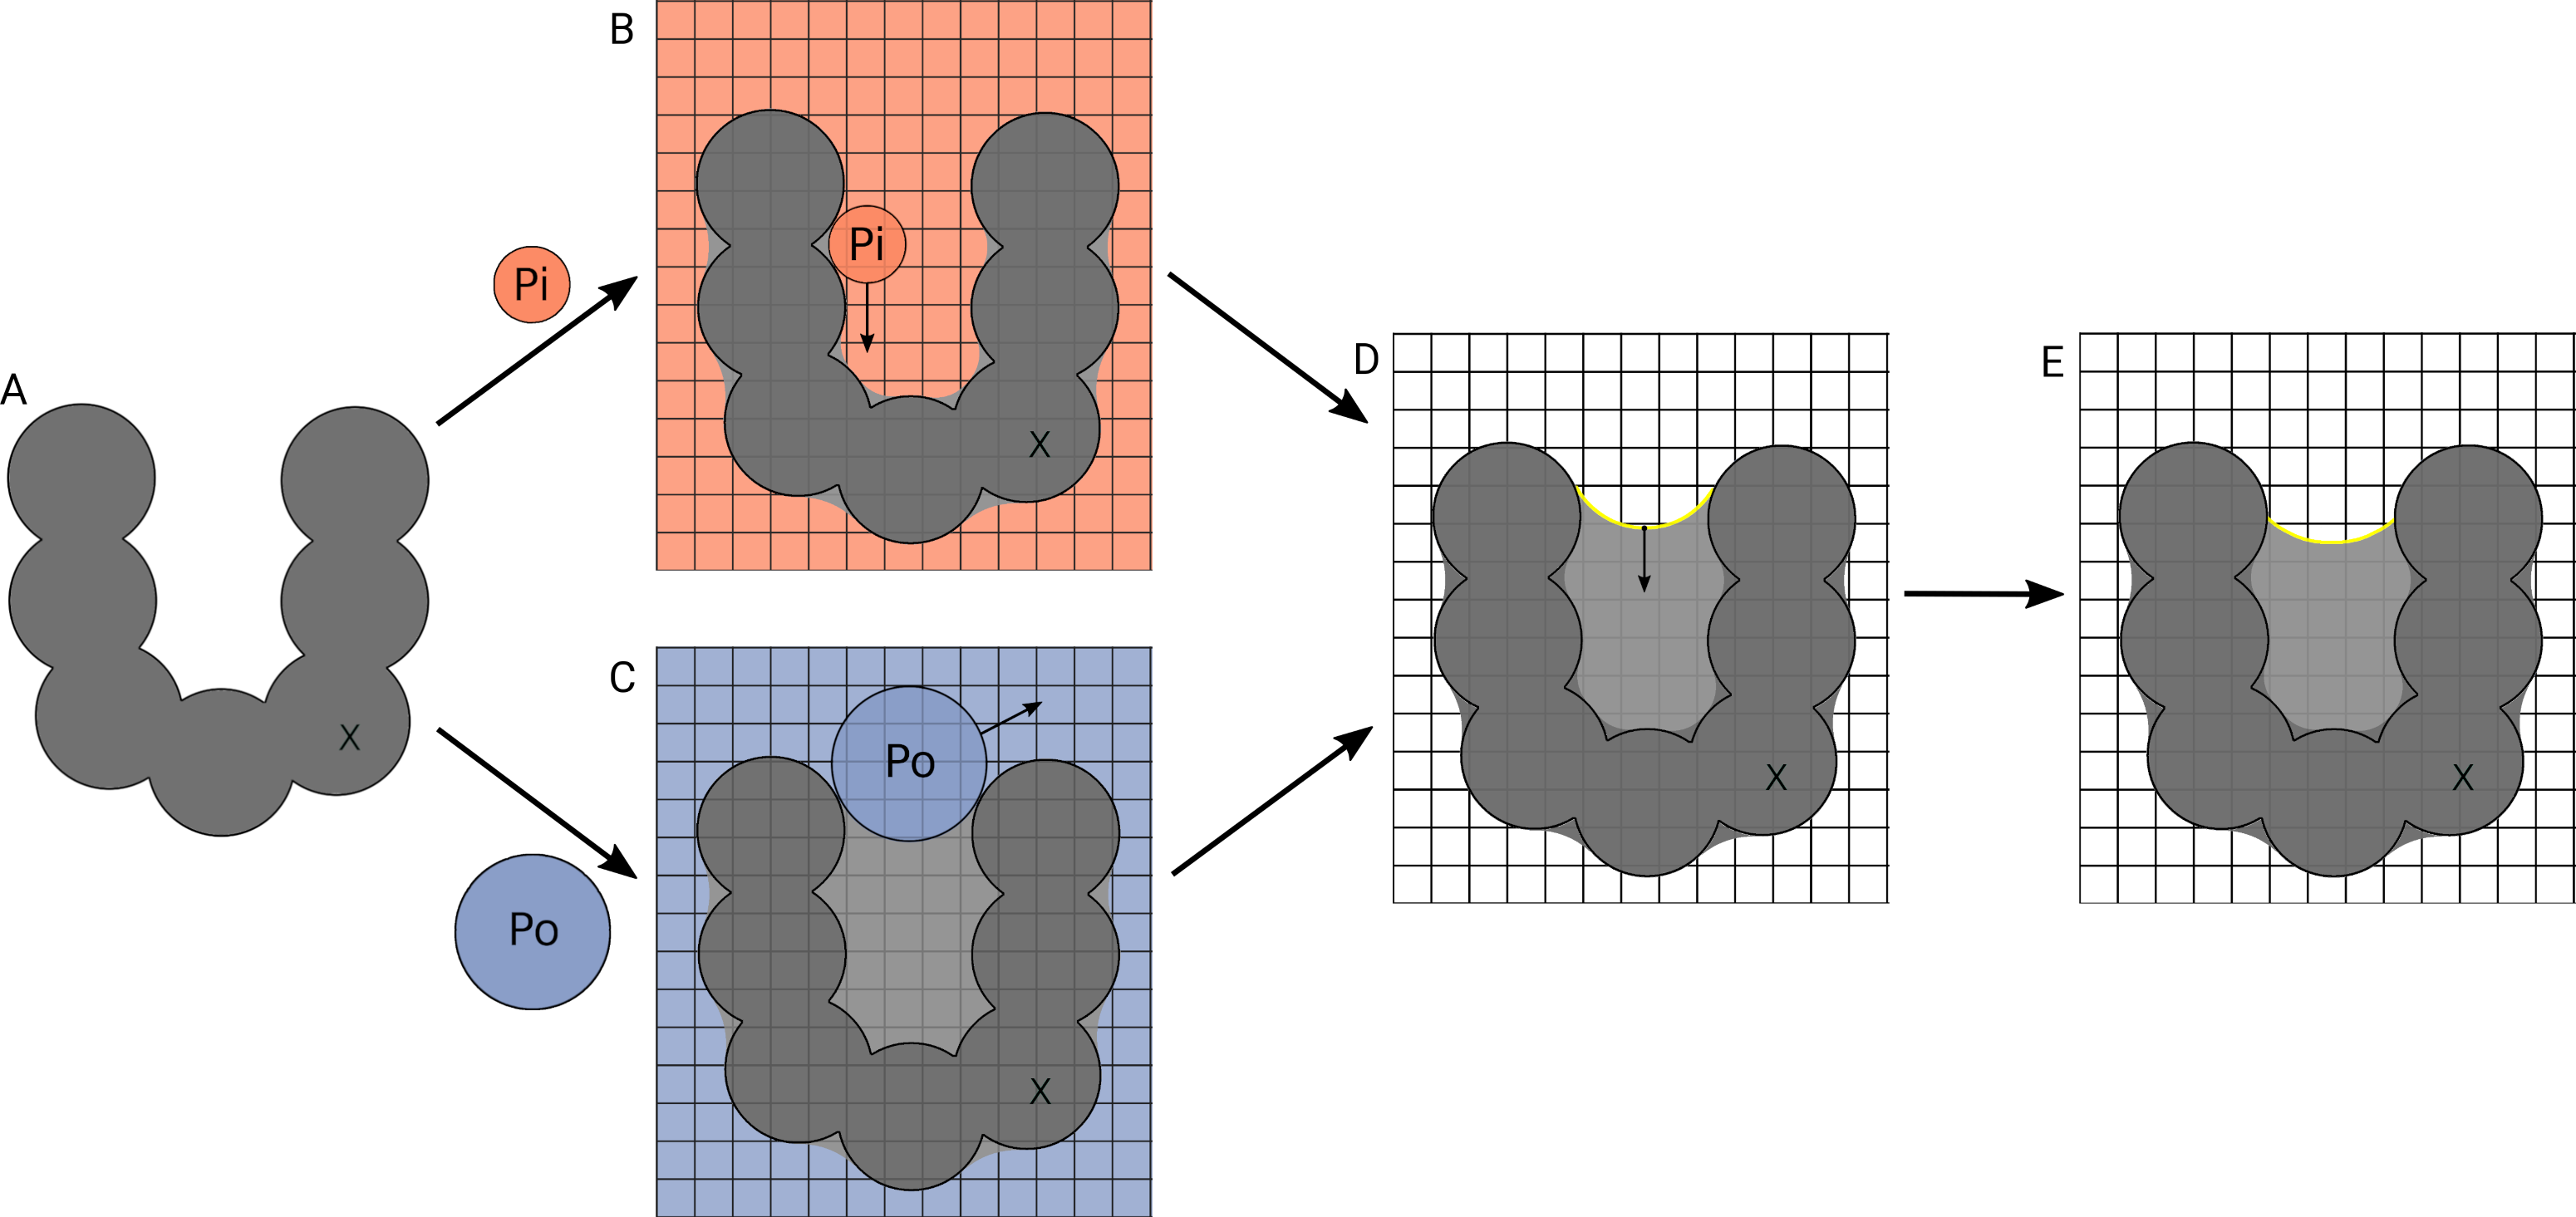
\includegraphics[scale=0.65]{images/kvfinder-suite-schema.png}}
  \centerline{\scriptsize{\textbf{Fonte:} Retirado de \cite{guerra2023B}.}}
  \caption[Representação esquemática do algoritmo de detecção de cavidades no KVFinder suite]{\textbf{Representação esquemática do algoritmo de detecção de cavidades no KVFinder suite.} \textbf{(A)} Uma estrutura biomolecular X, composta por átomos modelados como esferas rígidas com raios de van der Waals, é inserida em uma grade 3D. \textbf{(B)} A sonda \textit{Probe In} (Pi) percorre a superfície da estrutura, movendo-se pelos pontos da grade (laranja). \textbf{(C)} Em seguida, a sonda \textit{Probe Out} (Po) percorre os pontos acessíveis em azul. \textbf{(D)} Os pontos de cavidade (cinza claro) são definidos como a diferença entre os pontos acessíveis das sondas. Os pontos não alcançados por Pi (cinza escuro) definem a SES (padrão) ou a SAS, dependendo da representação de superfície escolhida pelo usuário. \textbf{(E)} Por fim, é aplicado um procedimento de remoção por distância para eliminar os pontos de cavidade que estão próximos à fronteira da cavidade-solvente (linha amarela).}
  \label{fig:kvfinder-suite-schema}
\end{figure}

É importante destacar que a ferramenta KVFinder \cite{oliveira2014}, originalmente publicada em 2014, está descontinuada. No entanto, novas implementações foram desenvolvidas para aprimorar o desempenho computacional e a usabilidade, resultando nas ferramentas parKVFinder \cite{guerra2020}, pyKVFinder \cite{guerra2021} e KVFinder-web \cite{guerra2023A}. Cada uma dessas ferramentas aborda diferentes demandas da comunidade científica de forma flexível. A caracterização das cavidades nessas ferramentas inclui descritores morfológicos, como volume, área, forma e profundidade, bem como descritores topológicos, como os resíduos de interface que cercam as cavidades, e descritores físico-químicos, como a hidrofobicidade. Para mais informações sobre o KVFinder suite, veja a Seção \ref{sec:kvfinder-suite}.

\subsubsection{Fpocket}

O Fpocket \cite{fpocket} é uma ferramenta baseada em tesselação que realiza a detecção de bolsões com base no conceito de \textalpha-esferas, introduzido por \cite{liang1998}. O algoritmo de detecção de cavidade (Figura \ref{fig:fpocket-schema}) determina o conjunto de \textalpha-esferas a partir da estrutura-alvo, utilizando o pacote \textit{qhull}, e elimina esferas fora de um tamanho de raio mínimo e máximo. As cavidades são agrupamentos de \textalpha-esferas, formadas com base em relações de proximidade e vizinhança, sendo que cavidades não interessantes são removidas da análise posterior. As cavidades restantes são avaliadas usando um conjunto de descritores dpocket \cite{fpocket} e classificadas de acordo com sua suposta capacidade de ligação a uma pequena molécula.

\begin{figure}[ht]
  \centerline{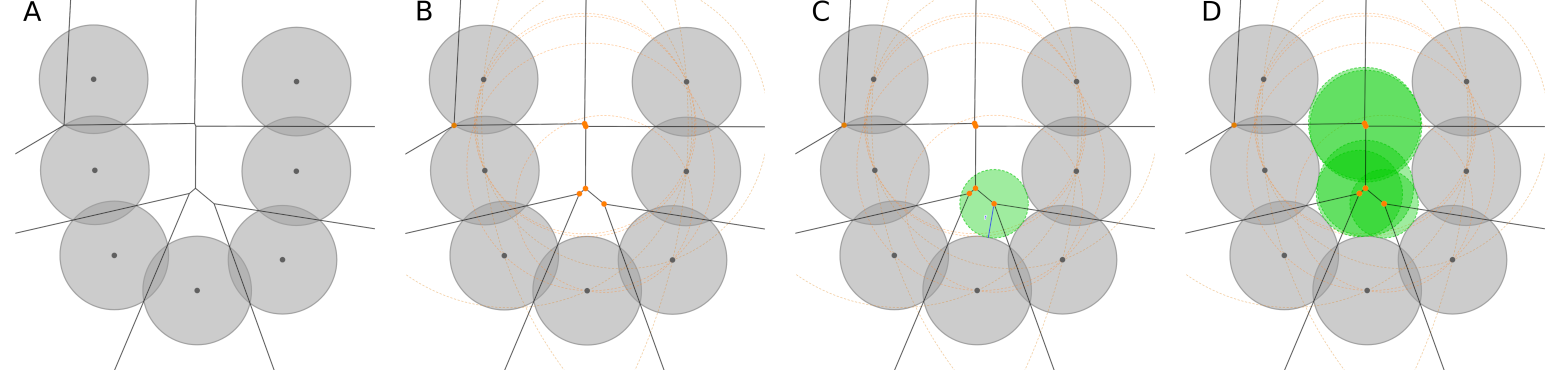
\includegraphics[scale=0.24]{images/fpocket-schema.png}}
  \centerline{\scriptsize{\textbf{Fonte:} Retirado de \cite{guerra2023B}.}}
  \caption[Representação esquemática do algoritmo de detecção de cavidades no Fpocket]{\textbf{Representação esquemática do algoritmo de detecção de cavidades no Fpocket.} \textbf{(A)} Diagrama de Voronoi dos centros atômicos. \textbf{(B)} Semelhante a uma esfera de Voronoi (círculos laranja pontilhados). \textbf{(C)} Exemplo de uma \textalpha-esfera (região verde); ela é centrada em um vértice de Voronoi (pontos laranja) e cresce até se tornar tangente aos átomos da superfície. \textbf{(D)} Cluster de \textalpha-esferas que preenchem o sítio de ligação.}
  \label{fig:fpocket-schema}
\end{figure}

\subsubsection{GHECOM}

O GHECOM (\textit{Grid-based HECOMi finder}) \cite{ghecom} é uma ferramenta baseada em grade e esfera que detecta bolsos profundos e rasos, utilizando várias sondas esféricas diferentes (Figura \ref{fig:ghecom-schema}). O algoritmo de detecção de cavidade combina operações básicas de erosão e dilatação, da morfologia matemática, com diferentes sondas esféricas para relatar a abertura-fechamento de uma forma molecular-alvo, revelando assim bolsos profundos e rasos (\textit{multi-scale pockets}, em inglês). Dessa forma, um método de agrupamento de ligação simples agrupa regiões de bolsos e posteriormente estima seus volumes. Além disso, o GHECOM relaciona o volume e a profundidade de pontos por resíduo ou átomo em uma métrica chamada \textit{pocketness}, que indica o quanto eles contribuem para a interação com ligantes.

\begin{figure}[ht]
  \centerline{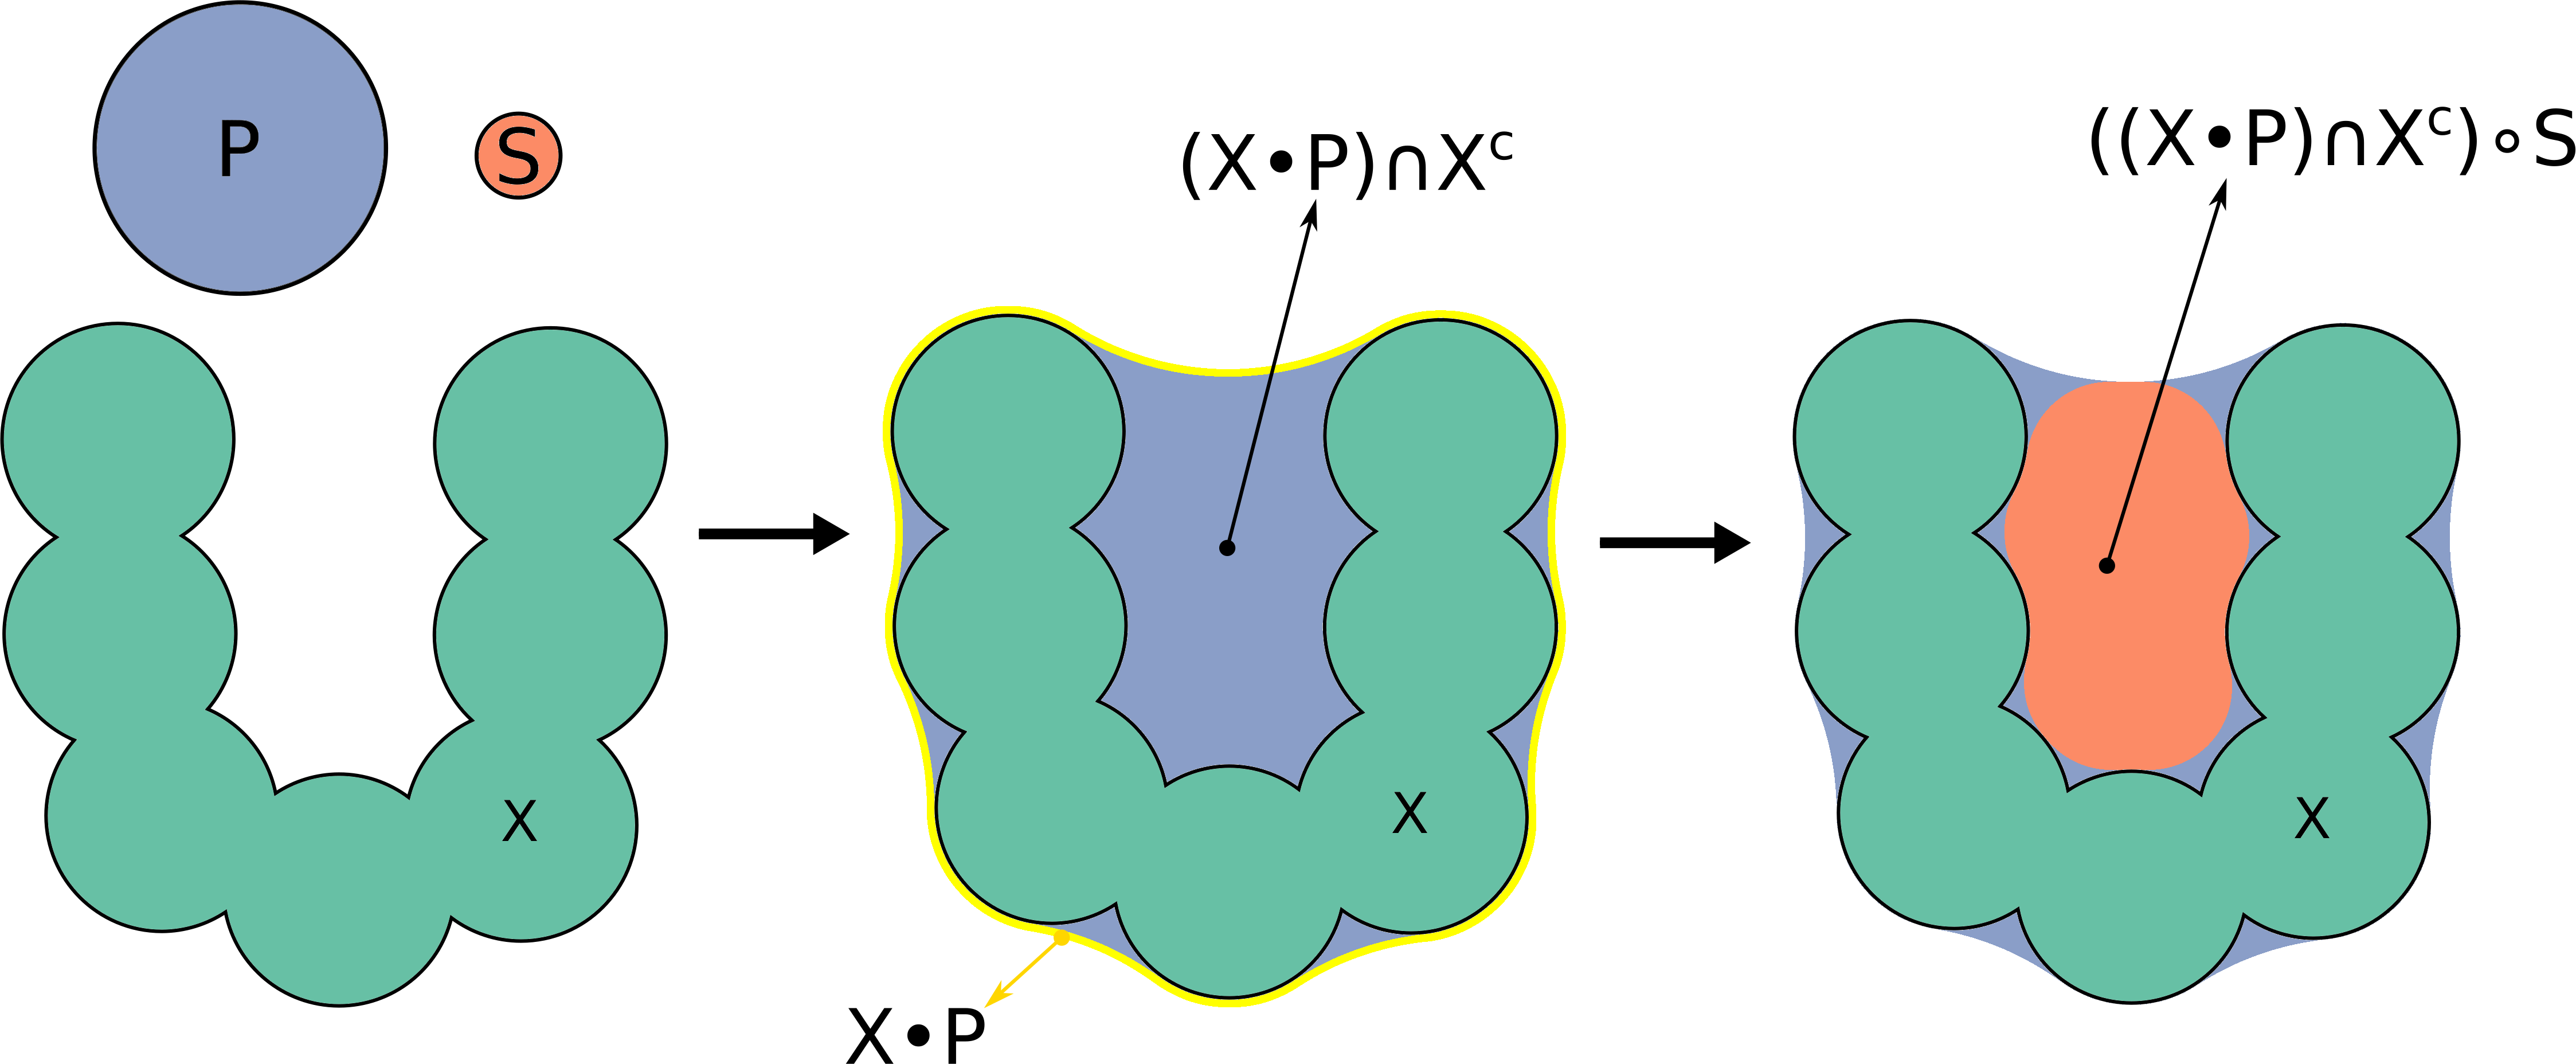
\includegraphics[scale=0.6]{images/ghecom-schema.png}}
  \centerline{\scriptsize{\textbf{Fonte:} Retirado de \cite{guerra2023B}.}}
  \caption[Representação esquemática do algoritmo de detecção de bolsões no GHECOM]{\textbf{Representação esquemática do algoritmo de detecção de bolsões no GHECOM.} Uma estrutura biomolecular (região verde; $X$) é fechada por uma sonda esférica P (esfera azul), definindo a região delimitada pelo contorno amarelo. Em seguida, a interseção de X fechado por P ($X \bullet P$) e o espaço fora da proteína ($X^c$) define a região não acessível à sonda P (região azul; $(X \bullet P) \cap X^c$). Posteriormente, essa região é aberta por uma sonda esférica S (esfera laranja), onde P é maior que S. Por fim, o bolsão (região laranja; $((X \bullet P) \cap X^c) \circ S$) é definido pelo espaço fora da forma molecular não acessível a P, mas acessível a S. Para detecção em múltiplas escalas, são usados diferentes tamanhos da sonda esférica P.}
  \label{fig:ghecom-schema}
\end{figure}

\subsubsection{CAVER}

O CAVER \cite{caver} foi originalmente uma ferramenta baseado em grade e superfície para o cálculo de túneis e canais, que posteriormente foi aprimorado no CAVER 3.0 \cite{caver3}, substituindo a grade alinhada aos eixos por uma abordagem de diagrama de Voronoi. A interface gráfica do usuário, CAVER Analyst 2.0 \cite{caveranalyst2}, incorpora o CAVER 3.0, que auxilia visualmente os usuários nos cálculos de túneis e cavidades. O algoritmo de detecção de cavidades (Figura \ref{fig:caver-schema}) constrói um pseudo-diagrama de Voronoi de uma estrutura biomolecular alvo. A partir dele, o CAVER 3.0 identifica caminhos como grafos compostos por vértices e arestas de Voronoi. Esses caminhos se assemelham a túneis que conectam cavidades ao solvente circundante e são caracterizados por comprimento, raio médio e raio do gargalo. Além disso, CAVER Analyst 2.0 também identifica regiões de espaço vazio, onde uma sonda pequena pode entrar de fora, mas uma sonda grande não pode, aplicando uma abordagem similar às descritas no KVFinder suite (Figura \ref{fig:kvfinder-suite-schema}) e GHECOM (Figura \ref{fig:ghecom-schema}).

\begin{figure}[ht]
  \centerline{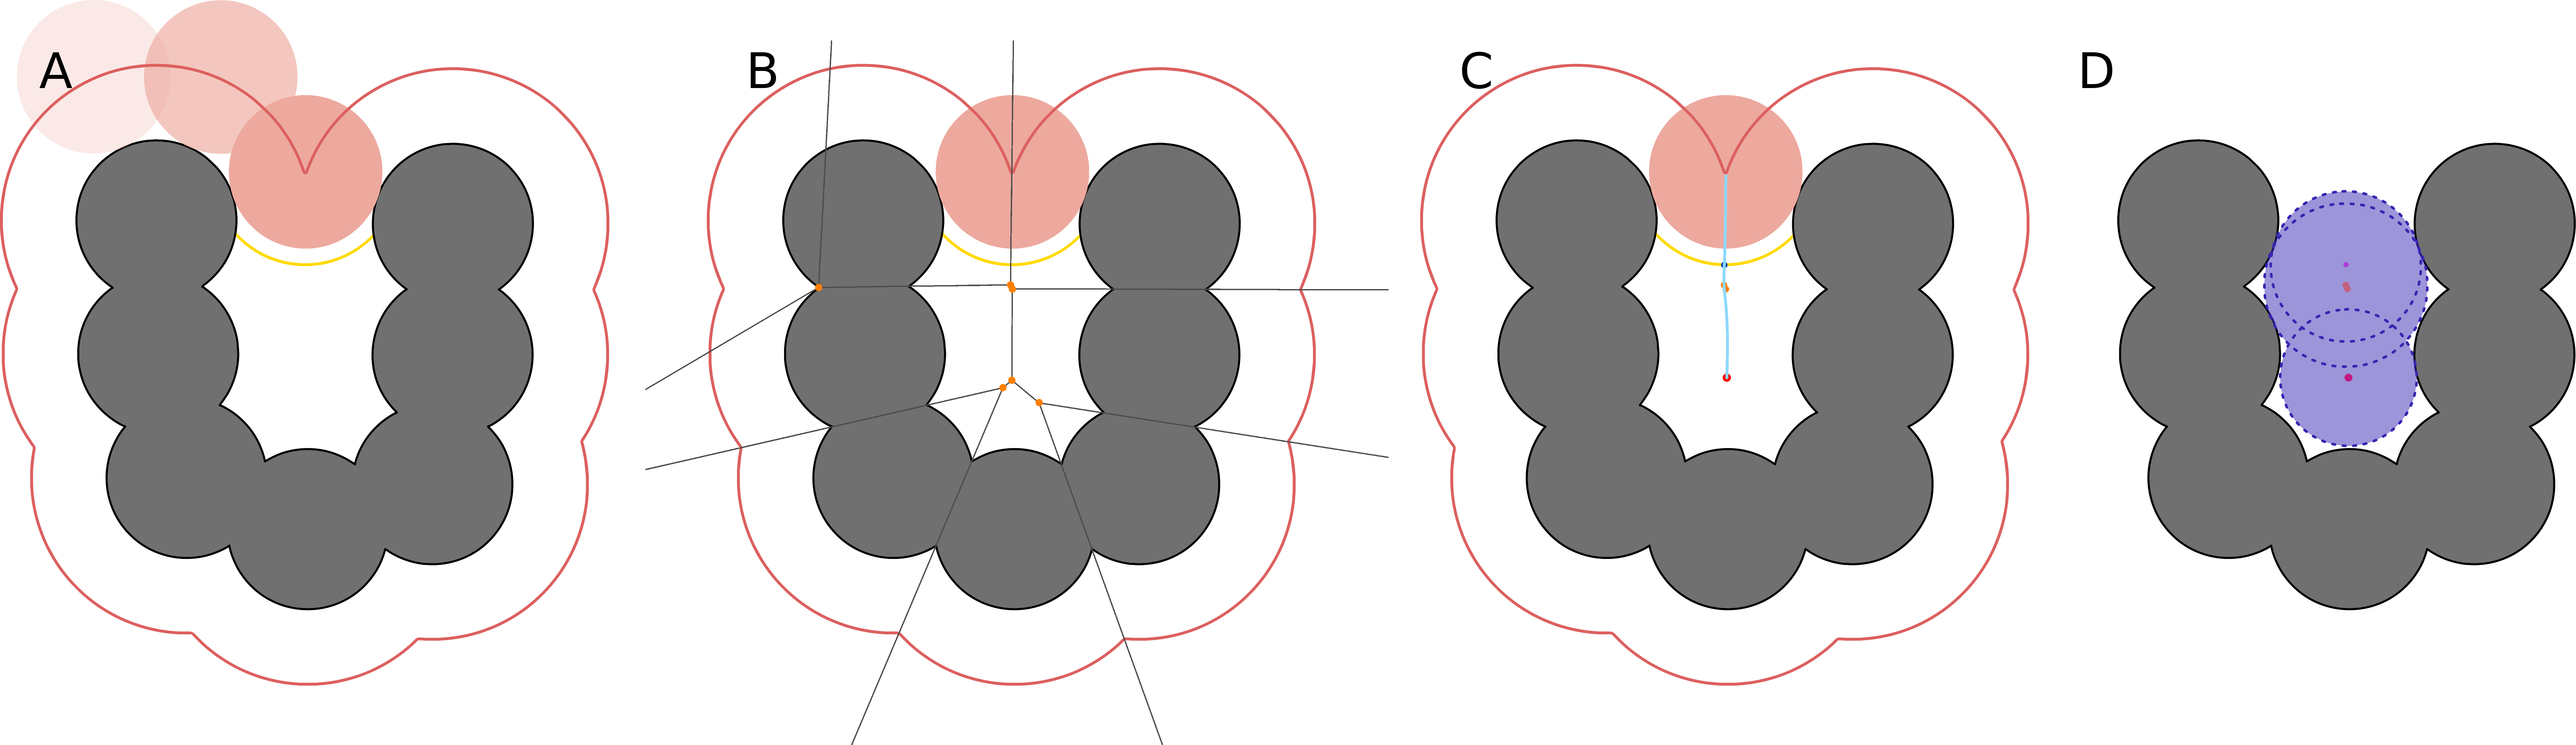
\includegraphics[scale=0.18]{images/caver-schema.png}}
  \centerline{\scriptsize{\textbf{Fonte:} Retirado de \cite{guerra2023B}.}}
  \caption[Representação esquemática do algoritmo de detecção de canais e túneis no CAVER 3.0 e CAVER Analyst 2.0]{\textbf{Representação esquemática do algoritmo de detecção de canais e túneis no CAVER 3.0 e CAVER Analyst 2.0.} \textbf{(A)} Uma forma molecular é inspecionada por uma sonda esférica, chamada \textit{shell probe}, com um raio especificado pelo parâmetro \textit{shell radius}, para definir uma superfície externa SAS (linha vermelha). A partir dela, uma distância especificada pelo parâmetro \textit{shell depth} é removida para definir uma superfície interna (linha amarela). \textbf{(B)} Um pseudo-diagrama de Voronoi é construído com base na forma molecular. Vértices de Voronoi (pontos laranja) são usados para criar as linhas centrais do túnel/canal. \textbf{(C)} Um ponto de partida (ponto vermelho) é um parâmetro definido pelo usuário, definido como o centro de massa da forma molecular, e um ponto final (ponto azul) é definido no centro da superfície interna. A partir do ponto de partida, a linha central passa por arestas e vértices de Voronoi para formar um túnel/canal até a superfície externa e passa pelo ponto final. \textbf{(D)} Esferas são ajustadas em todos os pontos da linha central, do ponto de partida ao ponto final, o que define o raio do gargalo (abertura) ao longo do túnel e/ou canal.}
  \label{fig:caver-schema}
\end{figure}

% Melhorias para a Defesa:
% - Caracterização de cavidades: describe importance of cavity characterization to identify functionally relevant cavities and how to do it

%%% Chapter 2

\chapter{Objetivos}

\section{Objetivo geral}

Este trabalho tem como objetivo o desenvolvimento de uma plataforma computacional, denominada \textbf{KVFinder suite}, para estudo de sistemas biomoleculares em biologia estrutural.

\section{Objetivos específicos}

% \begin{itemize}
%   \item Aprimoramento e desenvolvimento de descritores de propriedades do KVFinder suite;
%   \item Implementação de diferentes codificações para biomoléculas e sítios de ligação; % cavidade, resíduos e grafos
%   \item Desenvolvimento de ferramenta para ciência de dados e protocolos automatizados; % pyKVFinder
%   \item Desenvolvimento de um serviço \textit{web} para análise de sítios de ligação; % KVFinder-web
%   \item Desenvolvimento de ferramenta para análises dinâmica molecular; % KVFinderMD
%   \item Desenvolvimento de um programa para representação gráfica de regiões expostas de biomoléculas. % SERD
% \end{itemize}

Os objetivos específicos incluem: (1) Aprimoramento e desenvolvimento de descritores de propriedades do KVFinder suite; (2) Implementação de diferentes codificações para biomoléculas e sítios de ligação; (3) Desenvolvimento de ferramenta para ciência de dados e protocolos automatizados; (4) Desenvolvimento de um serviço \textit{web} para análise de sítios de ligação; (5) Desenvolvimento de ferramenta para análises dinâmica molecular; e (6) Desenvolvimento de um programa para representação em forma de grafos de interface de interação de biomoléculas.

%%% Chapter 3

\chapter{Codificação de biomoléculas e seus sítios de ligação}

% \begin{itemize}
%   \item Explique as diferentes representações de biomoléculas que podem ser usadas em simulações computacionais e em estudos de sítios de ligação;
%   \item Descreva em detalhes as representações usadas no KVFinder suite, como modelos de pontos, modelos de esferas, superfícies moleculares e mapas de densidade eletrônica;
%   \item Explique como cada uma dessas representações pode ser usada para identificar sítios de ligação em biomoléculas.
%  \end{itemize}

A codificação de biomoléculas e sítios de ligação desempenha papel fundamental na biologia estrutural, permitindo a representação e análise computacional de informações biológicas complexas. Esse processo converte informações biológicas em formatos compreensíveis e adequados para processamento por algoritmos e programas em sistemas computacionais. A codificação envolve a atribuição de valores ou categorias aos componentes biológicos, \eg, átomos, aminoácidos e bases nitrogenadas, para descrever ocupância, localização, forças, características físico-químicas e/ou propriedades estruturais. 

Na biologia estrutural, a codificação de dados é importante para realizar análises avançadas, \eg modelagem molecular, simulações de dinâmica molecular e predição de interações. Existem várias aplicações que exemplificam a codificação de dados biológicos para análises computacionais. Por exemplo, na modelagem molecular, uma proteína pode ser codificada usando códigos de uma letra para representar os diferentes aminoácidos, como ocorre na representação de sequência de proteínas, para predizer o dobramento de proteínas, como aplicado no ESMFold \cite{lin2022}. Na simulação de dinâmica molecular, as coordenadas 3D de átomos ou conjunto de átomos, juntamente com vetores que representam forças ou outros atributos, são utilizados para representar a estrutura de uma biomolécula, como no GROMACS \cite{gromacs} ou AMBER \cite{amber} em simulações em escala atomística (\textit{fine-grained molecular dynamics simulation}, em inglês) e no CafeMol em simulações em escala grosseiras (\textit{coarse-grained molecular dynamics simulation}, em inglês) \cite{kenzaki2011}. Além disso, os sítios de ligação, após identificados por algoritmos computacionais, são codificados de diferentes maneiras para análises posteriores. Os sítios de ligação podem codificados para representar as características físico-químicas e estruturais de uma região de uma biomolécula, como as grades 3D utilizadas no KVFinder suite \cite{oliveira2014,guerra2020,guerra2021,guerra2023B}, ou as coordenadas 3D dos átomos, como no fpocket \cite{fpocket}.

Ao trabalhar com modelos computacionais para o estudo de biomoléculas, a codificação é essencial para a abstração e representação dos dados biológicos de forma computacional. Essa abstração é crucial para o desenvolvimento de ferramentas computacionais voltadas ao estudo de sistemas biomoleculares. Aqui, apresentamos as codificações implementadas para biomoléculas e sítios de ligação, \ie, representação em grade 3D, representação topológica e representação em grafos.

\section{Representação em grade tridimensional}

As biomoléculas e seus sítios de ligação podem ser representadas em uma grade 3D subdividida em voxels (\textit{volumetric pixel}, em inglês). A grade 3D é uma estrutura de dados que armazena valores em uma matriz tridimensional, onde cada elemento da matriz é denominado voxel. O voxel representa um ponto discreto de dados em uma grade regular no espaço tridimensional, sendo que cada ponto pode conter mais de uma informação a fim de representar diferentes propriedades em uma certa porção de espaço de maneira simples e efetiva (Figura \ref{fig:voxel}). Em computação, a grade 3D é uma estrutura de dados comumente utilizada em aplicações de processamento de imagens e visão computacional, como em reconstrução de imagens, segmentação de imagens e detecção de objetos. 

\begin{figure}[ht]
  \centerline{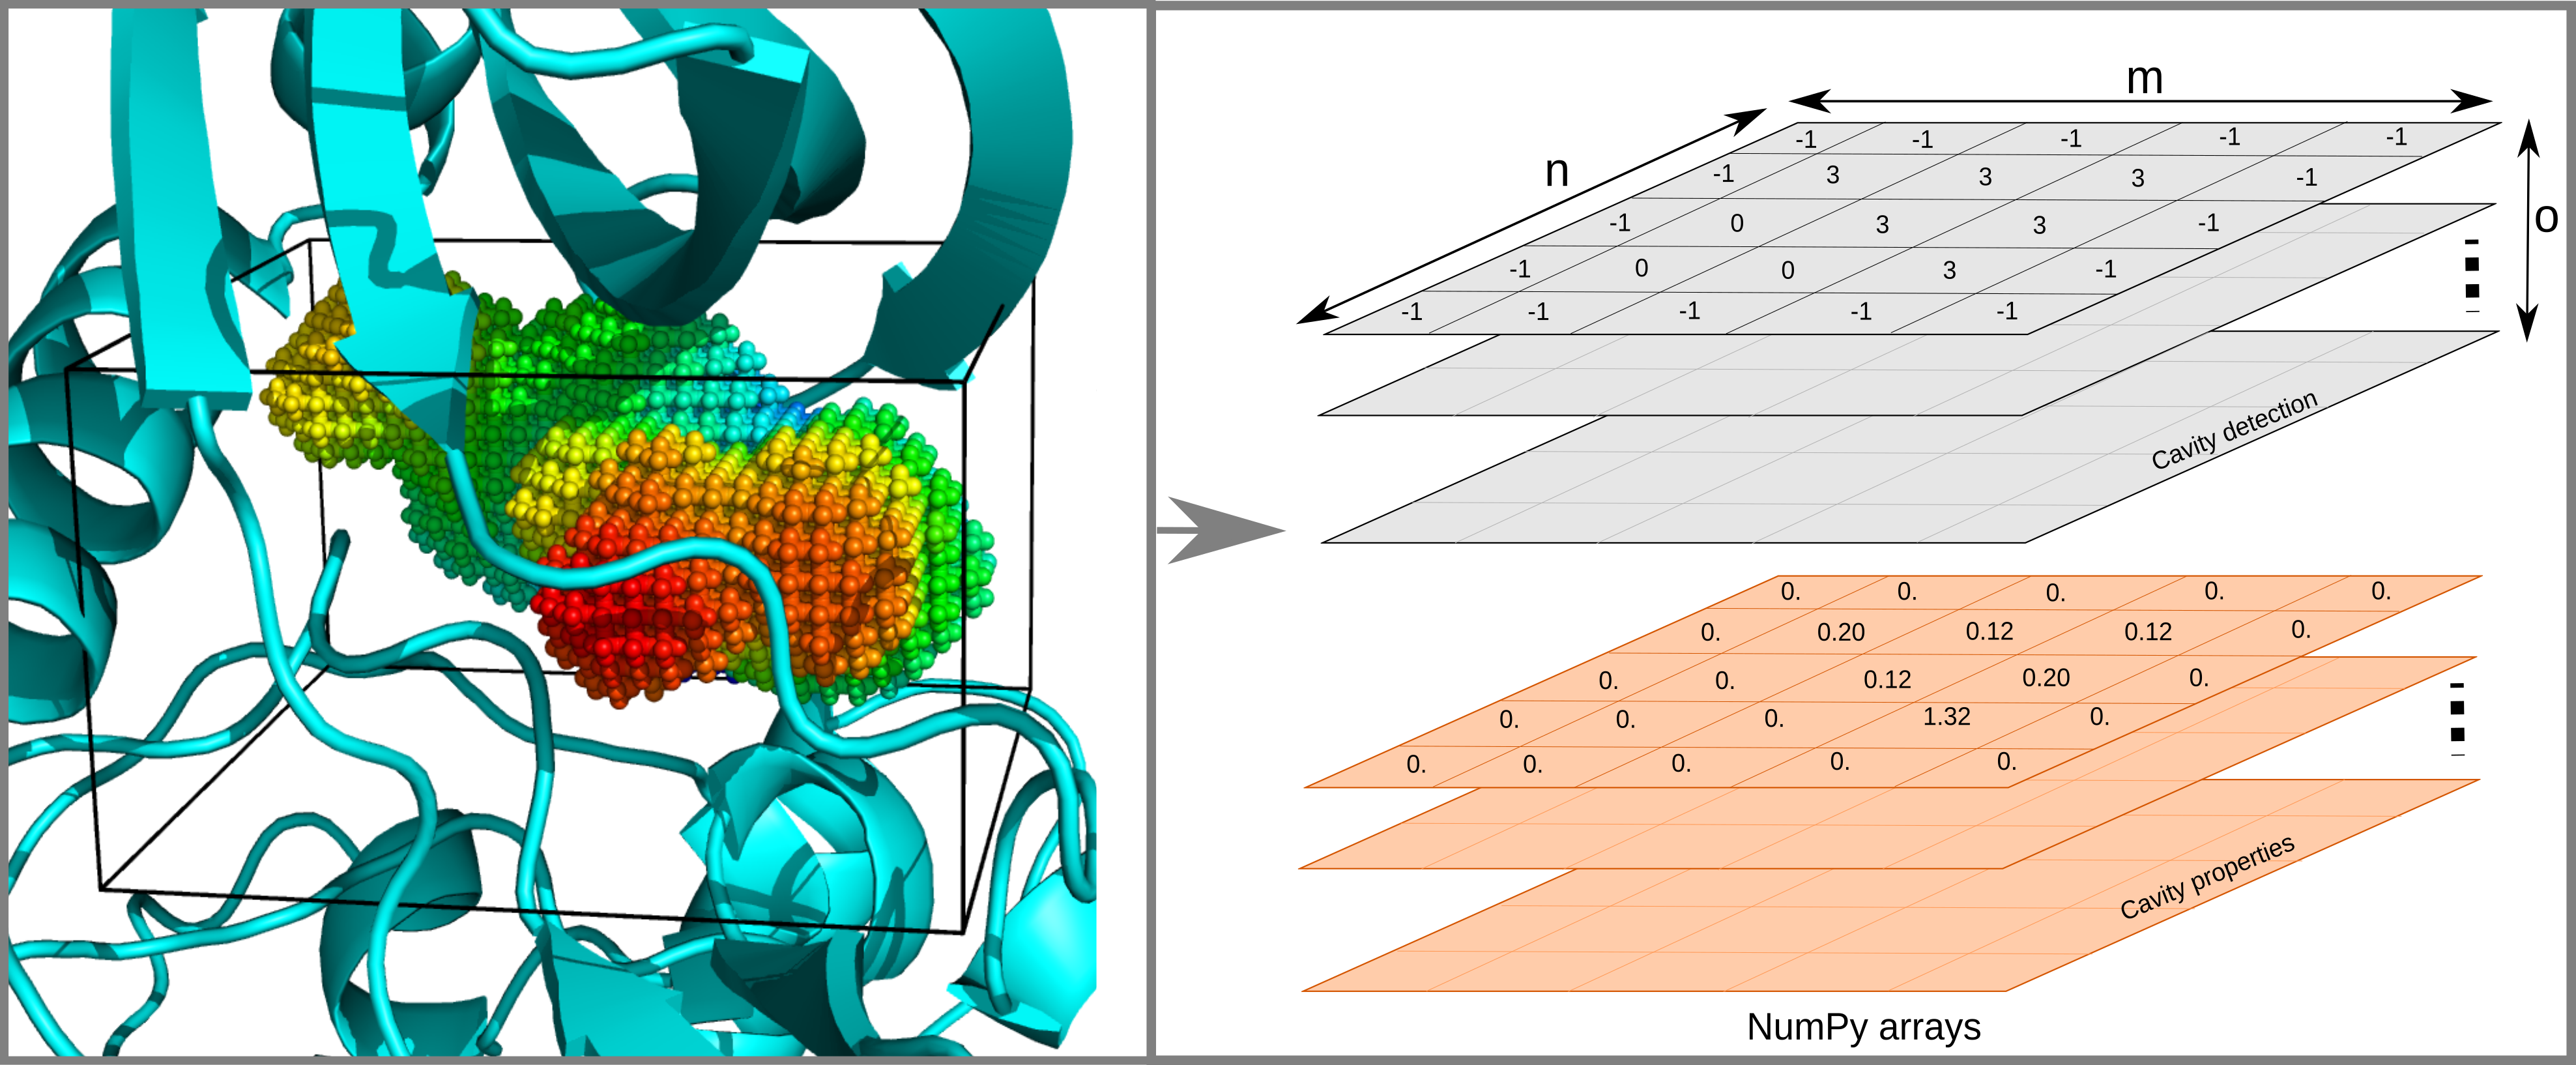
\includegraphics[scale=0.75]{images/voxels.png}}
  \centerline{\scriptsize{\textbf{Fonte:} Retirado de \cite{guerra2021}.}}
  \caption[Representação esquemática de biomoléculas e seus sítios de ligação representadas em grade tridimensional]{\textbf{Representação esquemática de biomoléculas e seus sítios de ligação representadas em grade tridimensional.} Com base em uma grade tridimensional com dimensões (m, n, o), cada elemento corresponde a uma região de cavidade (>1), espaço vazio (1), biomolécula (0) ou solvente (-1). Além disso, propriedades também são armazenadas na mesma estrutura de dados, correspondendo ao valor da propriedade na região.}
  \label{fig:voxel}
\end{figure}

Dentre as diversas representações de superfície molecular, a grade tridimensional composta por voxels é a mais simples e apropriada para a representação de múltiplas propriedades em várias condições, pois cada voxel da grade tridimensional pode acumular diferentes informações. Além disso, a grade 3D é uma estrutura de dados eficiente para armazenar e acessar valores e/ou atributos em uma posição 3D, permitindo a realização de operações matemáticas e lógicas em uma região 3D. 

% Essa representação é útil para identificar regiões de interesse em biomoléculas, como sítios de ligação, e para realizar análises de propriedades físico-químicas e estruturais, como a distribuição de cargas e a distribuição de propriedades hidrofóbicas. 

\subsection{Representação de superfícies moleculares}

A representação de superfícies moleculares é uma etapa fundamental na modelagem e análise de biomoléculas. Nessa abordagem, as biomoléculas são descritas por meio de um modelo de esfera rígida, que considera as posições e raios atômicos para representar a superfície molecular. Existem três formulações matemáticas comumente utilizadas para representar as superfícies moleculares (Figura \ref{fig:surface-representation}):

\begin{enumerate}[label=\textbf{(\Alph*)}]
  \item \textbf{superfície de vdW:} representa cada átomo por uma esfera cujo raio é proporcional ao seu raio de van der Waals. A superfície de vdW é representada como a união desses átomos esféricos; 
  \item \textbf{SAS:} representa as regiões de uma molécula que podem ser acessadas por uma molécula de solvente (\eg, uma molécula de água), que é aproximada por uma sonda esférica;
  \item \textbf{SES:} é semelhante ao SAS, mas considera-se a casca externa da sonda, em vez do centro da sonda.
\end{enumerate}

\begin{figure}[ht]
  \centerline{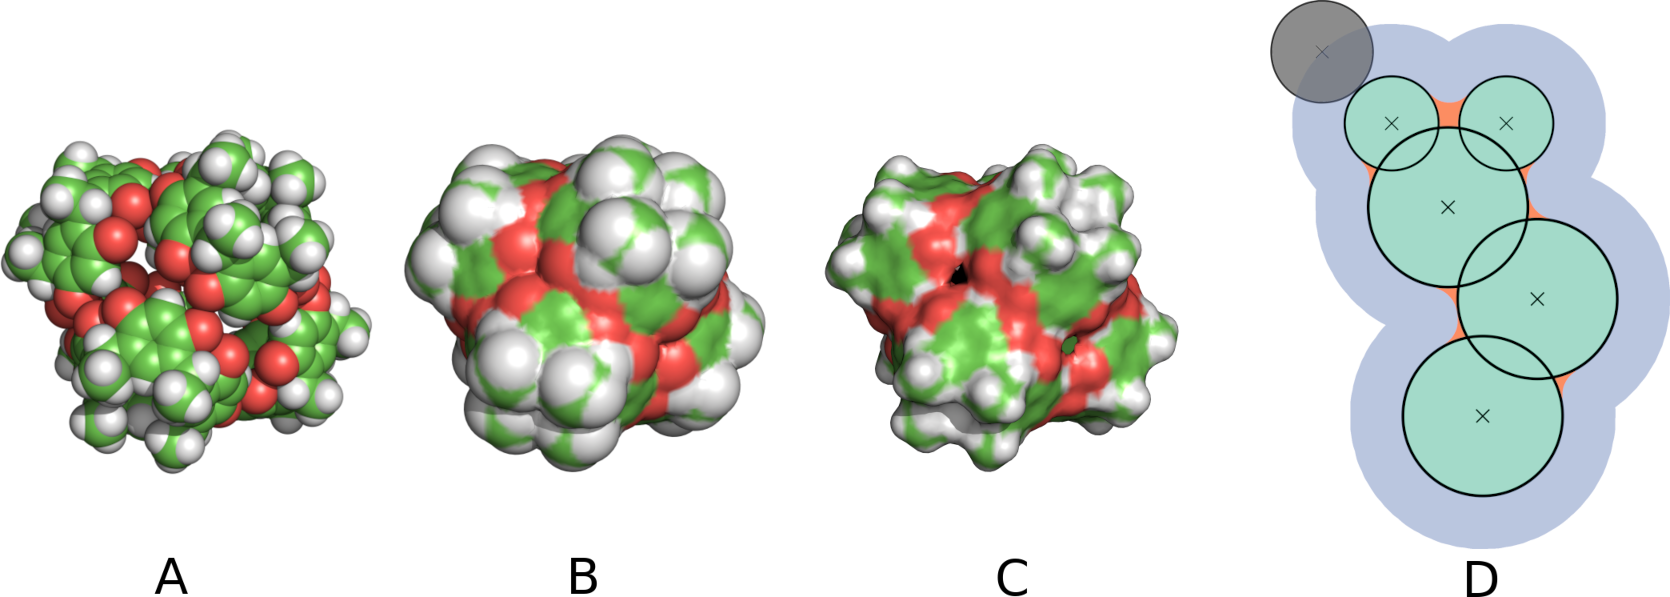
\includegraphics[scale=0.8]{images/surface-representation.png}}
  \centerline{\scriptsize{\textbf{Fonte:} Retirado de \cite{guerra2023B}.}}
  \caption[Representações de superfície molecular]{\textbf{Representações de superfície molecular.} \textbf{(A)} Superfície de vdW. \textbf{(B)} SAS. \textbf{(C)} SES. Imagens geradas com PyMOL para a gaiola supramolecular (resorcin[4]areno-hexamérica). \textbf{(D)} Representação esquemática 2D das superfícies moleculares. A superfície de vdW (verde) é composta por átomos representados como esferas verdes. Uma sonda esférica (cinza), representando uma molécula de solvente, rola sobre os átomos da molécula para definir SES e SAS. O SES é definido pela superfície de vdW (verde) e pelo espaço não alcançado pela sonda esférica (laranja). O SAS é definido pelo envelope alcançado pelo centro da sonda esférica (azul).}
  \label{fig:surface-representation}
\end{figure}

\section{Representação pela topologia}

% Melhorias para a Defesa:
% - Descrever implementação: Lista de listas (em Python) com informações sobre átomos, aminoácidos e/ou bases nitrogenadas.

Em vez de representar os dados estruturais por meio de voxels em uma grade 3D, as biomoléculas e seus sítios de ligação também podem ser representados por sua topologia (Figura \ref{fig:topology-representation}), seguindo abordagens semelhantes às simulações de dinâmica molecular, como GROMACS \cite{gromacs}, AMBER \cite{amber} e CafeMol \cite{kenzaki2011}. Nessa representação, átomos, resíduos e/ou bases nucleotídicas são modelados como esferas rígidas (\textit{hard sphere models}, em inglês) com coordenadas 3D (x, y, z), juntamente com vetores (\eg, forças, velocidades e acelerações) e propriedades (\eg, massa, carga e raio de vdW).

\begin{figure}[ht]
  \centerline{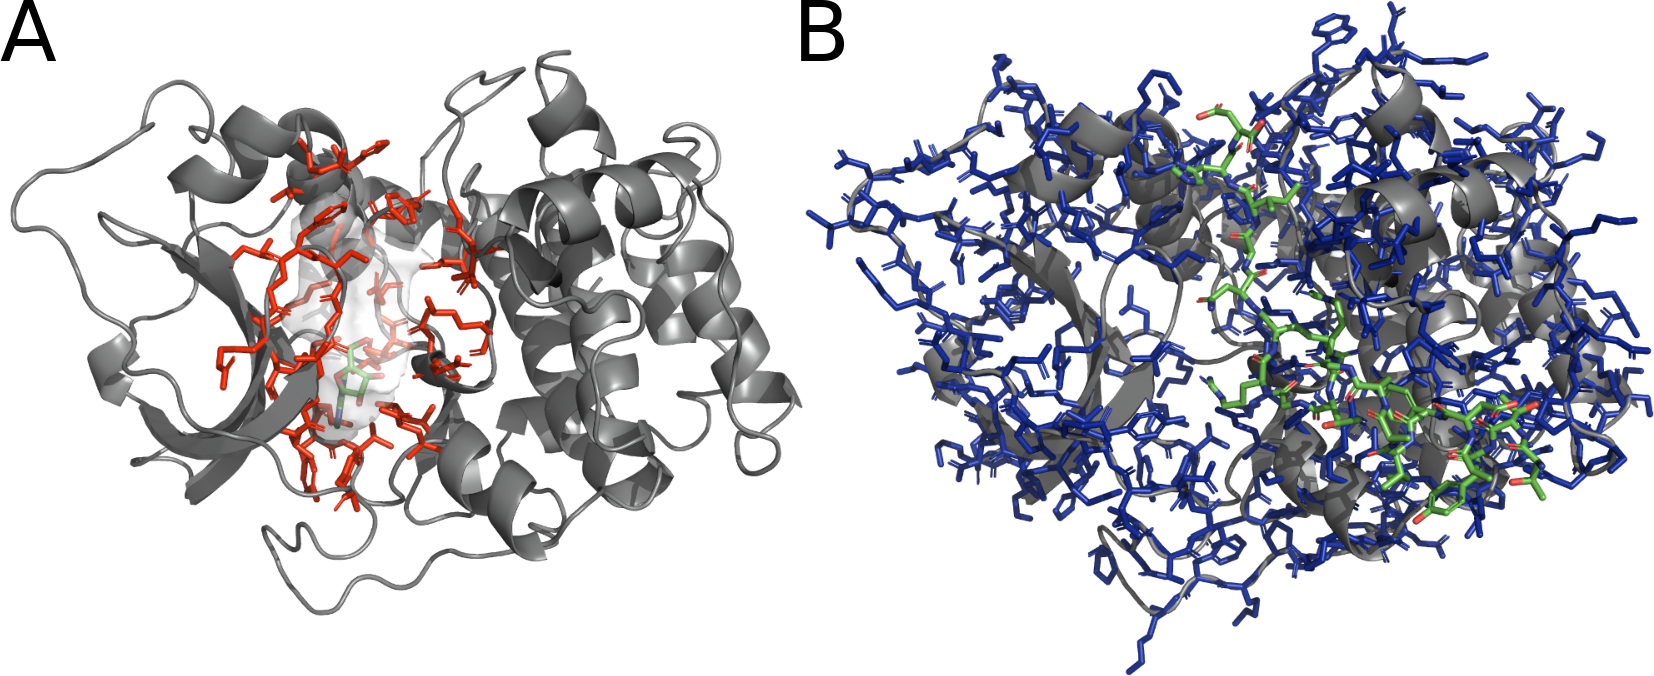
\includegraphics[scale=2]{images/topology-representation.png}}
  \caption[Representações topológicas de interfaces de interação em estruturas biomoleculares]{\textbf{Representações topológicas de interfaces de interação em estruturas biomoleculares.} \textbf{(A)} Átomos e aminoácidos (\textit{sticks} em verde) que formam o sítio de ligação da adenosina (superfície transparente). \textbf{(B)} Átomos e aminoácidos (\textit{sticks} em azul) expostos ao solvente, que excluem sítios de ligação para pequenas moléculas, com um inibidor ligado (\textit{sticks} em verde). Imagens geradas com PyMOL para uma subunidade da proteína quinase CAMP-dependente (PDB ID: 1FMO).}
  \label{fig:topology-representation}
\end{figure}

Porém, ao estudarmos regiões de interação, é necessário filtrar as áreas de interesse, como sítios de ligação (Figura \ref{fig:topology-representation}A) ou superfície exposta ao solvente (Figura \ref{fig:topology-representation}B), para realizar análises estruturais e funcionais específicas. Essa representação topológica permite análises direcionadas, focando nas interações e características estruturais relevantes para a função biológica. Além disso, as informações topológicas podem ser utilizadas em estudos de acoplamento molecular (\textit{molecular docking}, em inglês), desenho racional de fármacos e predição de interações moleculares. Essas aplicações contribuem para o desenvolvimento de novos compostos terapêuticos e auxiliam na compreensão dos mecanismos moleculares envolvidos em processos biológicos.

Dessa forma, a representação topológica das biomoléculas e seus sítios de ligação proporciona uma visão detalhada e especializada das características estruturais relevantes, permitindo uma análise mais precisa e aprofundada das interações moleculares e seu impacto na função biológica.

\section{Representação em grafos}

% Melhorias para a Defesa:
% - Figura de grafos genéricos para a Defesa
% - Expandir sobre os tipos de grafos: direcionados, não-direcionados, ponderados, etc.
% - Expandir sobre as propriedades em vértices e arestas
% - Expandir sobre as aplicações de grafos em biologia

A representação de interações ou relações entre elementos por meio de grafos é uma abordagem que tem sido utilizada em diversas áreas, como biologia, química, física, ciência da computação e matemática \cite{foulds1995,majeed2020}. Grafos são estruturas de dados poderosas e flexíveis que podem ser usadas para representar e analisar relações e interações entre elementos. No contexto de biomoléculas, essa representação já foi utilizada para investigar a estrutura, dobramento, estabilidade, função e dinâmica de proteínas \cite{vishveshwara2002}.

Grafos são estruturas matemáticas compostas por um conjunto de vértices (também chamados de nós) e um conjunto de arestas que conectam esses vértices. No caso de moléculas, que são conjuntos de átomos (vértices) conectados por interações intramoleculares e intermoleculares (arestas), também têm sido amplamente investigadas pela teoria dos grafos \cite{vishveshwara2002,mason2007}.

A representação de grafos implementada utiliza as coordenadas 3D (x, y, z) de uma estrutura ou complexo biomolecular e gera um grafo de resíduos, onde os vértices representam os resíduos e as arestas representam interações ou algum tipo de relação entre eles. A construção das arestas é baseada em cortes de distância customizáveis entre os átomos, como carbono \textalpha, carbono \textbeta\space ou qualquer outro átomo, que podem ser definidos pelo usuário (Figura \ref{fig:graph-representation}). Os parâmetros padrões definidos na implementação são uma distância de corte de 10 Å entre átomos carbono \textalpha, de 8 Å entre átomos carbono \textbeta\space (ou carbono \textalpha\space para glicina), e de 5 Å entre quaisquer dois átomos são estabelecido para definir relação ou interação entre resíduos, respectivamente \cite{vishveshwara2002,mason2007}. A Figura \ref{fig:graph-representation}A mostra um exemplo de grafo de resíduos gerado a partir de um sítio de ligação da adenosina (Figura \ref{fig:topology-representation}A) e a Figura \ref{fig:graph-representation}B mostra um exemplo de grafo de resíduos gerado a partir de uma superfície exposta ao solvente (Figura \ref{fig:topology-representation}B).

% Ref CB e all-atoms: https://www.ebi.ac.uk/msd-srv/capri/round28/round28.html

\begin{figure}[ht]
  \centerline{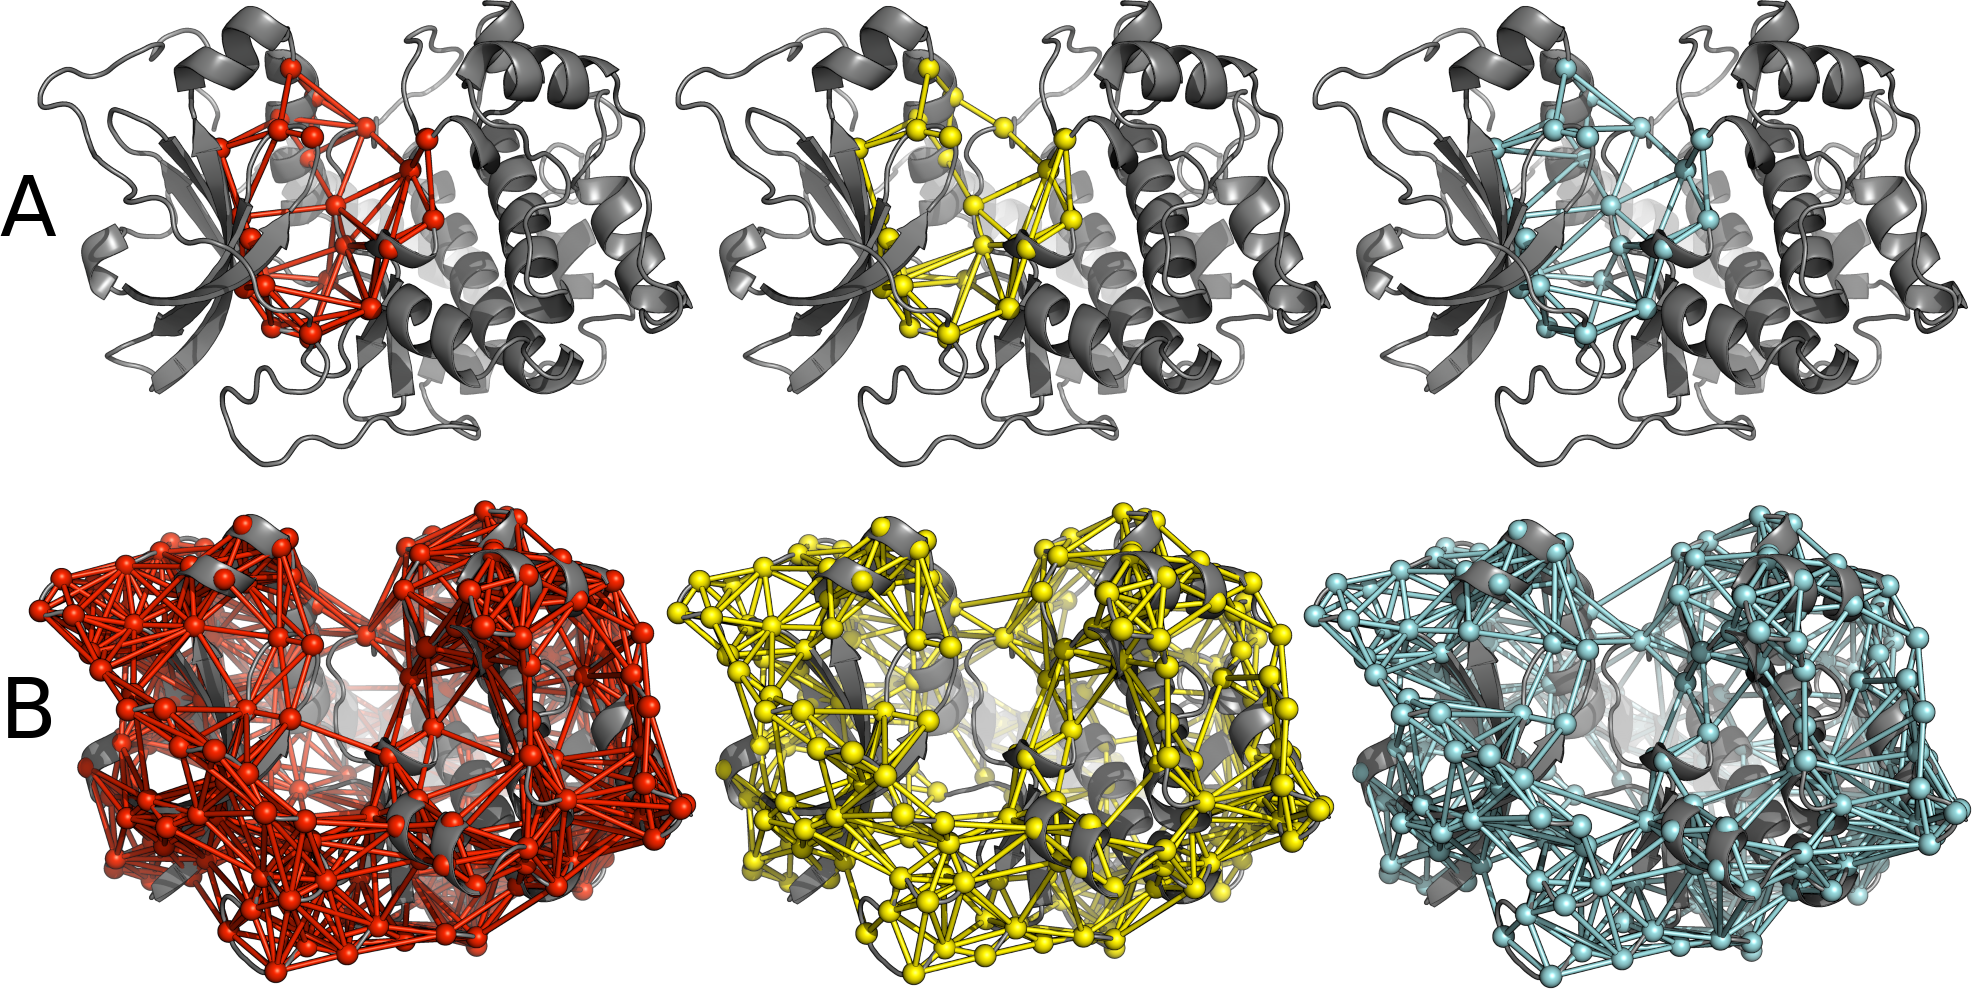
\includegraphics[scale=1.9]{images/graph-representation.png}}
  \caption[Representações em forma de grafos em estruturas biomoleculares]{\textbf{Representações em forma de grafos em estruturas biomoleculares.} \textbf{(A)} Sítio de ligação da adenosina como grafos com arestas baseados no corte de distância de carbono \textalpha\space (esferas e bastões em vermelho), carbono \textbeta\space (esferas e bastões em amarelo) e qualquer átomos dos resíduos (esferas e bastões em ciano). \textbf{(B)} Superfície exposta ao solvente, que excluem sítios de ligação para pequenas moléculas, como grafos com arestas baseados no corte de distância de carbono \textalpha\space (esferas e bastões em vermelho), carbono \textbeta\space (esferas e bastões em amarelo) e qualquer átomos dos resíduos (esferas e bastões em ciano). Imagens geradas com PyMOL para uma subunidade da proteína quinase CAMP-dependente (PDB ID: 1FMO).}
  \label{fig:graph-representation}
\end{figure}

Essa representação em grafos permite uma análise mais simplificada e eficiente das interações e relações entre os resíduos, proporcionando uma visualização clara das características estruturais e funcionais da biomolécula. Além disso, diversas propriedades e medidas podem ser calculadas a partir dos grafos, como caminhos, distâncias, centralidade e outras métricas que auxiliam na compreensão da estrutura e função da biomolécula \cite{majeed2020,vishveshwara2002,mason2007}. Em resumo, a representação em grafos é uma abordagem poderosa e versátil para analisar a estrutura e as interações em biomoléculas, permitindo uma compreensão mais aprofundada de sua função biológica e fornecendo \textit{insights} importantes para o desenvolvimento de terapias e intervenções terapêuticas.

%%% Chapter 4

\chapter{Plataforma KVFinder suite \label{sec:kvfinder-suite}}

% \begin{itemize}
%   \item Descreva cada um dos programas do KVFinder suite, explicando seus objetivos e principais características;
%   \item Apresente exemplos de aplicação de cada programa em estudos de sítios de ligação em biomoléculas, mostrando os resultados obtidos e como eles contribuíram para a compreensão da função biológica das moléculas estudadas;
%   \item Explique como os resultados obtidos pelo KVFinder suite podem ser validados experimentalmente.
%  \end{itemize}

% https://cnpemcamp-my.sharepoint.com/:w:/r/personal/joao_guerra_lnbio_cnpem_br/_layouts/15/Doc.aspx?sourcedoc=%7BD0C80180-AF7E-412F-B94E-6C38D8D4C946%7D&file=Relat%C3%B3rio%20Plataforma%20Biologia%20Computacional%202022.2.docx&action=default&mobileredirect=true

As interações entre biomoléculas desempenham um papel crucial em processos biológicos, envolvendo desde pequenas moléculas, como íons e fármacos, até macromoléculas, como proteínas e ácidos nucleicos. Essas interações receptor-ligante (\eg, IPPs, IPLs, IPRs e IPDs) ocorrem em sítios de ligação específicos, que podem ser fendas expostas ao solvente ou cavidades enterradas nos receptores. A complementariedade espacial, estrutural e físico-química entre os ligantes e receptores governa o reconhecimento molecular, restringindo a interação eficiente a um número limitado de ligantes. A identificação e avaliação dessas regiões são fundamentais para o entendimento da estrutura terciária da biomolécula e para o desenvolvimento de novos fármacos. Para atender a essa demanda, desenvolvemos a plataforma computacional \textbf{KVFinder suite}, que combina ferramentas precisas com processamento de alto desempenho, permitindo a análise de dados experimentais biomoleculares e a compreensão da estrutura e função das biomoléculas em sistemas biológicos.

A KVFinder suite é composta por cinco ferramentas computacionais que oferecem funcionalidades abrangentes para análise estrutural e estudo de interações biomoleculares. As ferramentas incluídas na plataforma são: parKVFinder \cite{guerra2020}, pyKVFinder \cite{guerra2021}, KVFinder-web \cite{guerra2023A}, KVFinderMD e SERD. A seguir, descreveremos cada uma dessas ferramentas e suas principais características.

\section{parKVFinder}

O \textbf{Parallel KVFinder (parKVFinder)} \cite{guerra2020} é uma ferramenta de código aberto, licenciada sob GPL v3.0, desenvolvida para detecção e caracterização de qualquer tipo de cavidade biomolecular. A ferramenta foi desenvolvida originalmente na dissertação de mestrado intitulada "Prospecção e caracterização de cavidades supramoleculares" \cite{guerra2019}, como uma versão atualizada e otimizada do KVFinder \cite{oliveira2014}. Posteriormente, o parKVFinder foi publicado na SoftwareX \cite{guerra2020}, aprimorando a estimativa de área superficial, sendo lançado como \href{https://github.com/LBC-LNBio/parKVFinder/tree/v1.0}{parKVFinder v1.0}. Em seguida, houve uma nova atualização para o KVFinder-web \cite{guerra2023A}, adicionando os descritores de profundidade, hidrofobicidade e frequência de resíduos, resultando no lançamento do \href{https://github.com/LBC-LNBio/parKVFinder/tree/v1.2.0}{parKVFinder v1.2.0}.

O parKVFinder é acompanhado por um plugin gráfico chamado \textit{PyMOL2 parKVFinder Tools}, que é integrado ao visualizador molecular PyMOL. Esse plugin oferece uma interface gráfica intuitiva e fácil de usar, permitindo que os usuários explorem parâmetros personalizáveis para a detecção e caracterização de cavidades. Além disso, o plugin permite visualizar as cavidades detectadas e suas características no ambiente do PyMOL. Além da interface gráfica, o parKVFinder também possui uma interface de linha de comando (CLI; \textit{command-line interface}) para usuários avançados, o que permite a automação de tarefas e a integração com outros programas. O código-fonte do parKVFinder e o plugin estão disponíveis no seguinte repositório: \url{https://github.com/LBC-LNBio/parKVFinder}.

As rotinas de detecção e caracterização de cavidades foram paralelizadas utilizando a biblioteca OpenMP, aproveitando o processamento paralelo em sistemas \textit{multicore}. O desempenho computacional do parKVFinder foi avalidado em um conjunto de 1000 domínios proteicos, denominado kv1000 (\url{https://github.com/jvsguerra/kv1000}), apresentando um tempo de execução consideravelmente menor que o KVFinder, aproximadamente 9.5 vezes mais rápido \cite{guerra2019,guerra2020}.

% Melhorias defesa:
% - Detalhar comparação com outros métodos
% - Detalhar atualização para Python3 do plugin

% O parKVFinder fornece detecção direcionada e caracterização topológica precisa, rápida e eficiente (forma, volume, área e resíduos circundantes), com uma paralelização multithread implementada com OpenMP. A detecção de cavidade depende de um conjunto de parâmetros personalizáveis e intuitivos, com os quais o usuário pode interagir por meio de uma interface gráfica (plugin para o PyMOL) ou de uma interface de linha de comando.

\subsection{Casos de estudo}

O parKVFinder foi aplicado em dois casos de estudo publicados em periódicos científicos para investigar proteínas de interesse terapêutico. Essas análises exploraram a dinâmica dos \textit{flaps} da HIV-1 protease \cite{guerra2020} e o caráter hidropático de sítios de ligação em alphavírus \cite{ribeiro2021}. A seguir, descreveremos cada um desses casos de estudo em detalhes.

\subsubsection{Dinâmica molecular da HIV-1 protease}

Nesse estudo, foi investigado a dinâmica molecular da HIV-1 protease por meio da identificação e avaliação do volume do sítio ativo durante simulações de dinâmica molecular (DM). O sítio ativo é um alvo terapêutico relevante e seu volume varia de acordo com a movimentação dos \textbeta-hairpins, conhecidos como \textit{flaps}, que controlam a acessibilidade do substrato ao sítio ativo do homodímero \cite{soares2016}. % Add more references here

O objetivo era descrever a dinâmica de movimentação dos \textit{flaps} através do volume e forma da cavidade do sítio ativo como descritores conformacionais durante as simulações de MD. Para isso, foram realizadas simulações de DM por 200 ns, usando o pacote GROMACS 2019.4 \cite{gromacs}, o campo de força AMBER99SB-ws e o modelo de água TIP42005s, partindo da estrutura cristalográfica da protease do HIV-1 na conformação fechada \cite{lam1994}, sem o inibidor.

O volume do sítio ativo foi acompanhado ao longo das simulações (Figura \ref{fig:hiv1-protease-dm-analysis}). Observou-se que o volume da cavidade começa no valor correspondente à conformação fechada (linha verde) e, após cerca de 25 ns, começa a aumentar até atingir o valor correspondente à conformação semi-aberta (linha vermelha) em cerca de 75 ns, indicando um processo de abertura ao longo da simulação. Posteriormente, os \textit{flaps} se afastam ainda mais, e a cavidade atinge seu volume máximo em cerca de 175 ns antes de reverter para a conformação semi-aberta, que é mais estável. Essa dinâmica de volume correlaciona-se (correlação de Pearson; $\rho = 0,72$) com o desvio médio quadrático (RMSD; \textit{Root-mean-square deviation}, em inglês) do C\textalpha\space calculado a partir da conformação fechada como referência, indicando uma descrição adequada do estado conformacional da proteína ao longo da simulação. É importante destacar que o RMSD é uma métrica que descreve variações globais na estrutura, enquanto o volume estimado é uma métrica direta das mudanças conformacionais do sítio ativo, possivelmente relacionadas à acessibilidade do ligante.

\begin{figure}[ht]
  \centerline{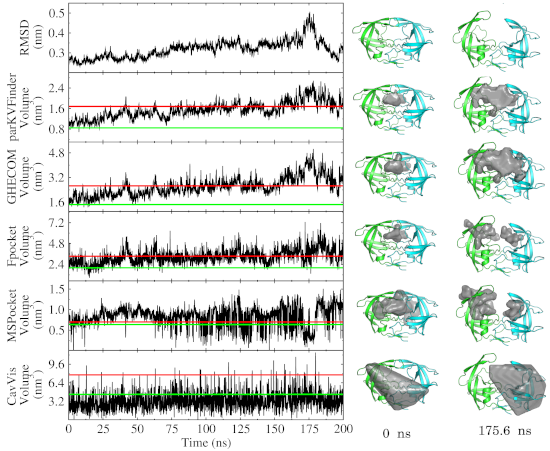
\includegraphics[scale=0.15]{images/hiv1-protease-md-analysis.png}}
  \caption[Volume de seu sítio ativo HIV-1 protease ao longo de uma simulação de dinâmica molecular de 200 ns]{\textbf{Volume de seu sítio ativo HIV-1 protease ao longo de uma simulação de dinâmica molecular de 200 ns.} As linhas verdes e vermelhas indicam o volume da cavidade para os estados fechado (PDB ID: 1HVR) e semi-aberto (PDB ID: 1HHP), respectivamente. As estruturas da proteína no início da simulação (0 ns) e no quadro com o maior RMSD (175.6 ns) são mostradas como diagramas. As cavidades correspondentes detectadas por cada software são mostradas como superfícies cinzas.}
  \label{fig:hiv1-protease-dm-analysis}
\end{figure}

% Caso necessário reduzir o tamanho do texto, pode-se remover ou resumir bem a comparação com outros métodos.

% Comparou-se o desempenho do parKVFinder \cite{guerra2020} com outros programas baseados em geometria (Figura \ref{fig:hiv1-protease-dm-analysis}), \ie, GHECOM \cite{ghecom}, Fpocket \cite{fpocket}, MSPocket \cite{mspocket} e CavVis \cite{cavvis}. Além da acurácia na descrição do estado conformacional do sítio ativo, também avaliou-se o tempo computacional dos programas. O parKVFinder apresentou alta acurácia, assim como o GHECOM, na descrição do estado conformacional da protease do HIV-1. No entanto, o parKVFinder mostrou-se pelo menos quatro vezes mais rápido que o GHECOM devido às subrotinas de múltiplas threads implementadas no parKVFinder. Além disso, o parKVFinder superou o MSPocket e o CavVis em termos de tempo computacional, mas não foi tão rápido quanto o Fpocket, que utiliza um método baseado em tesselação de Voronoi e esferas alfa. No entanto, a implementação do Fpocket mostrou-se menos sensível na descrição detalhada das cavidades da protease do HIV-1. Portanto, considerando a acurácia e o desempenho, o parKVFinder se destacou como uma opção robusta para a detecção e caracterização espacial de cavidades no caso de estudo da protease do HIV-1 \cite{guerra2020}.

Comparou-se o desempenho do parKVFinder \cite{guerra2020} com outros programas baseados em geometria (Figura \ref{fig:hiv1-protease-dm-analysis}), \ie, GHECOM \cite{ghecom}, Fpocket \cite{fpocket}, MSPocket \cite{mspocket} e CavVis \cite{cavvis}. Primeiramente, avaliou-se a correlação do volume estimado por cada programa e o RMSD, assim como realizado para o parKVFinder. O volume estimado pelo GHECOM ($\rho = 0,75$) também se correlaciona ao estado conformacional, semelhante ao parKVFinder ($\rho = 0,72$), possivelmente porque ambos empregam métodos baseados em grade e esfera. No entanto, as cavidades encontradas pelos programas Fpocket ($\rho = 0,35$), MSPocket ($\rho = -0,24$) e CavVis ($\rho = 0,19$) não apresentaram uma correlação satisfatória com a dinâmica conformacional do sítio ativo. Portanto, parKVFinder e GHECOM apresentaram uma alta acurácia na descrição do estado conformacional do sítio ativo da HIV-1 protease. 

Além de boa acurácia, também foi avaliado o tempo computacional dos programas. O parKVFinder ($t = 1h03m$) foi pelo menos quatro vezes mais rápido que o GHECOM ($t = 4h32m$), devido às subrotinas de múltiplas \textit{threads} implementadas no parKVFinder. Além disso, o parKVFinder também superou o MSPocket ($t = 2h48m$) e o CavVis ($t = 3h45$) em termos de tempo computacional, mas não superou o Fpocket ($t = 20m$), que utiliza um método baseado em tesselação de Voroni e esferas alfa, sendo rapidamente computado. No entanto, essa implementação do Fpocket mostrou-se menos sensível na descrição detalhada do sítio ativo da HIV-1 protease, não diferenciando eficientemente os estados conformacionais do sítio ativo. Portanto, considerando a acurácia e o desempenho, o parKVFinder destacou-se como uma opção robusta para a detecção e caracterização espacial de cavidades no caso de estudo da HIV-1 protease \cite{guerra2020}.

É importante ressaltar que os resultados completos e detalhes das simulações e análises estão disponíveis no artigo publicado no periódico \textit{SoftwareX} \cite{guerra2020}.

\subsubsection{Mayaro e outros alphavírus}

% Review it:
% - text, abbreviations and images

O vírus Mayaro (MAYV) é um arbovírus emergente das Américas Central e do Sul que pode causar uma doença debilitante e artritogênica. As proteínas E1 e E2 são importantes proteínas transmembranares organizadas em heterodímeros. Trímeros de heterodímeros de E1 e E2 compõem as espículas na superfície viral, que se estendem através da bicamada lipídica e interagem com as proteínas nucleocapsídicas C. As espículas estão envolvidas na ligação aos receptores celulares, internalização nas células e fusão de membrana. A liberação do RNA do MAYV no citoplasma resulta na expressão de proteínas virais, replicação viral e culmina na geração de progênie viral madura e infecciosa. As proteínas E1 e E2 do MAYV são os principais alvos para o desenvolvimento de vacinas e medicamentos antivirais \cite{ribeiro2021}. No entanto, a falta de informações estruturais sobre as proteínas E1 e E2 do MAYV tem dificultado o desenvolvimento de novas estratégias para combater a infecção pelo MAYV.

A região central entre as proteínas E1 e E2 forma uma cavidade que é ocupada por uma densidade extra longa, que não pode ser explicada por resíduos de cadeia lateral (Figura \ref{fig:mayv-e1-e2-analysis}A e B). Um perfil de densidade similar foi observado anteriormente em um mapa crioeletrônico do vírus Sindbis (SINV), e os autores propuseram que uma cauda fosfolipídica hidrofóbica (C18), chamada de \textit{pocket factor} (fator de bolsão, em português), poderia ocupar essa densidade e estabilizar o bolsão hidrofóbico formada entre E1 e E2 \cite{chen2018}.

\begin{figure}[t]
  \centerline{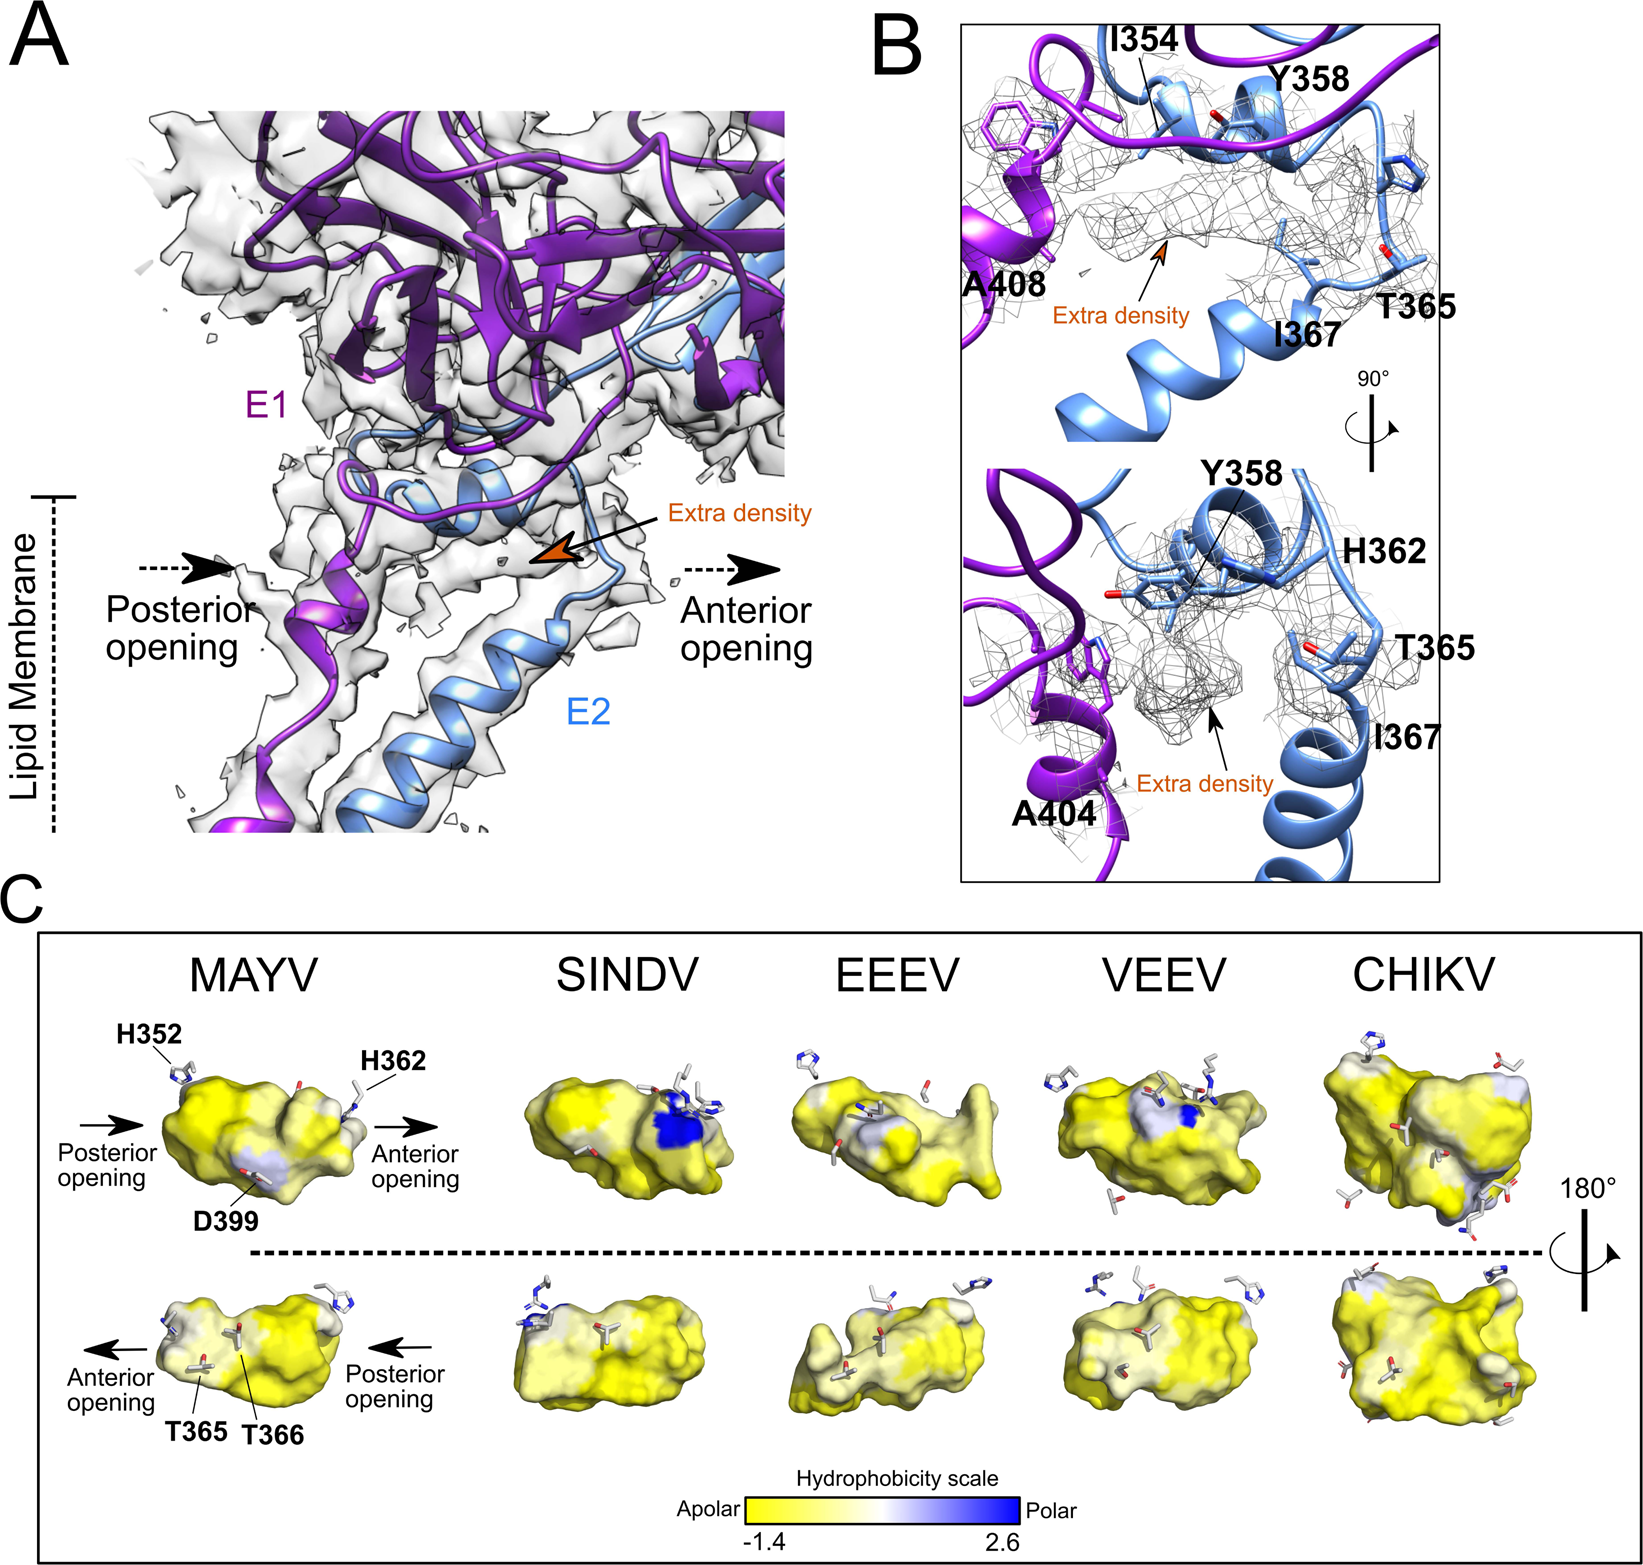
\includegraphics[scale=0.2]{images/mayv-e1-e2-analysis.png}}
  \caption[Domínios transmembranares E1 e E2 do MAYV e a cavidade hidrofóbica]{\textbf{Domínios transmembranares E1 e E2 do MAYV e a cavidade hidrofóbica.} \textbf{(A)} Modelo atômico 3D do MAYV ajustado ao mapa de densidade, mostrando a porção superior das hélices TM de E1 e E2. A interseção entre E1-E2 forma uma cavidade com abertura anterior e posterior. A densidade extra observada dentro da cavidade está indicada. \textbf{(B)} Detalhe da densidade extra encontrada na região da cabeça de E1-E2 e os resíduos ao redor. O mapa de densidade do MAYV está representado em superfície ou malha. \textbf{(C)} Prospeção da cavidade em estruturas de alphavírus. A cavidade entre os domínios E1 e E2 está representada em superfície e colorida com base na escala de consenso de Eisenberg, utilizando os resíduos que formam a cavidade, conforme detalhado na seção de métodos. Apenas os resíduos polares estão representados como sticks.}
  \label{fig:mayv-e1-e2-analysis}
\end{figure}

\begin{figure}[ht]
  \centering
    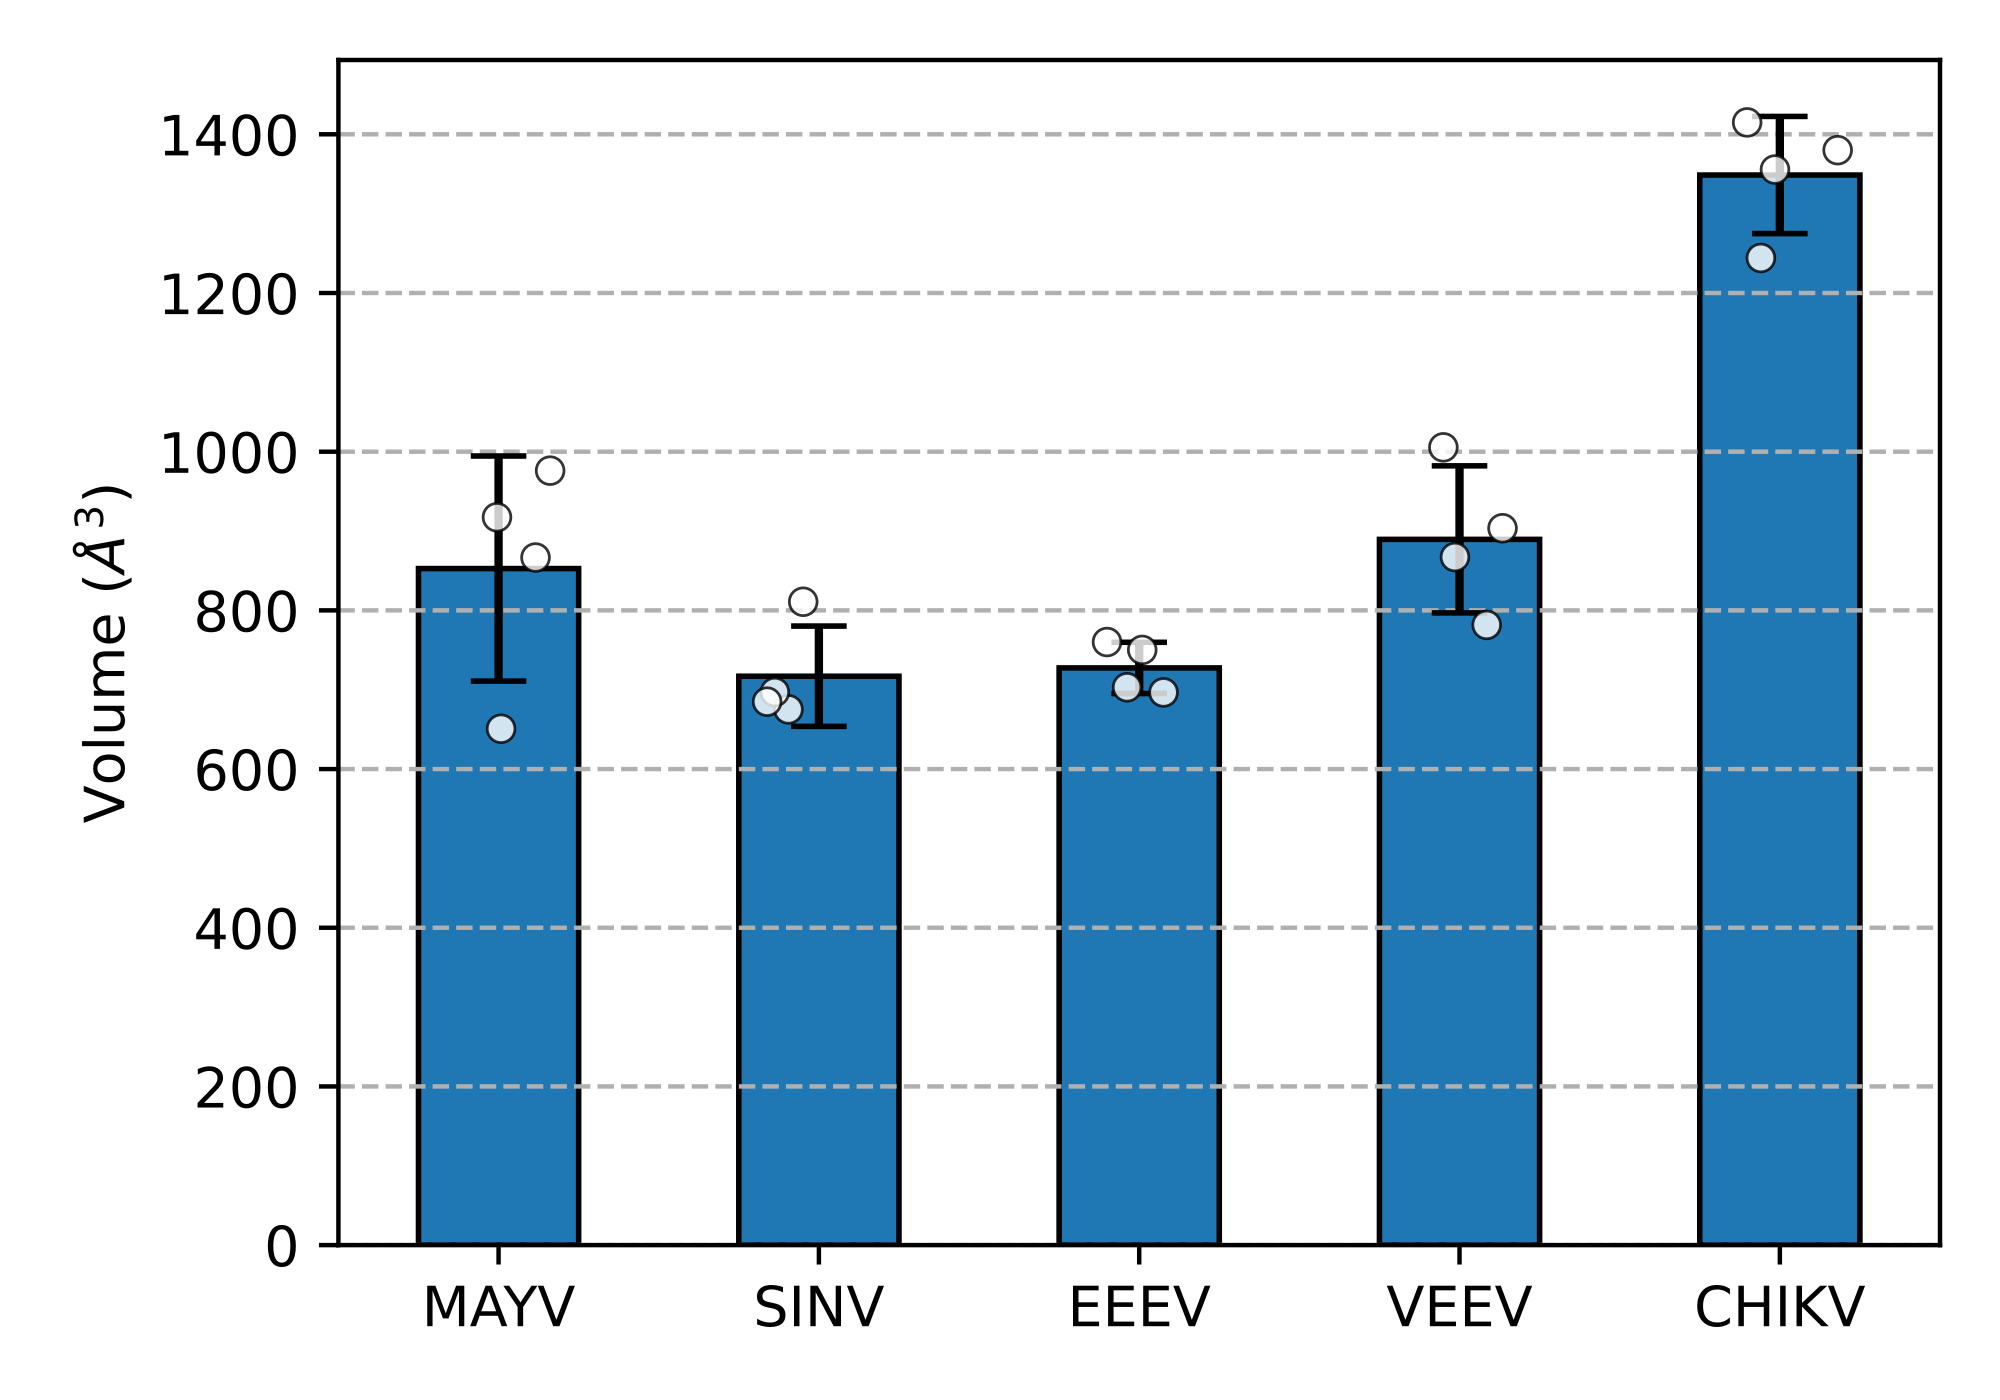
\includegraphics[scale=0.5]{images/mayv-e1-e2-volume.png}
    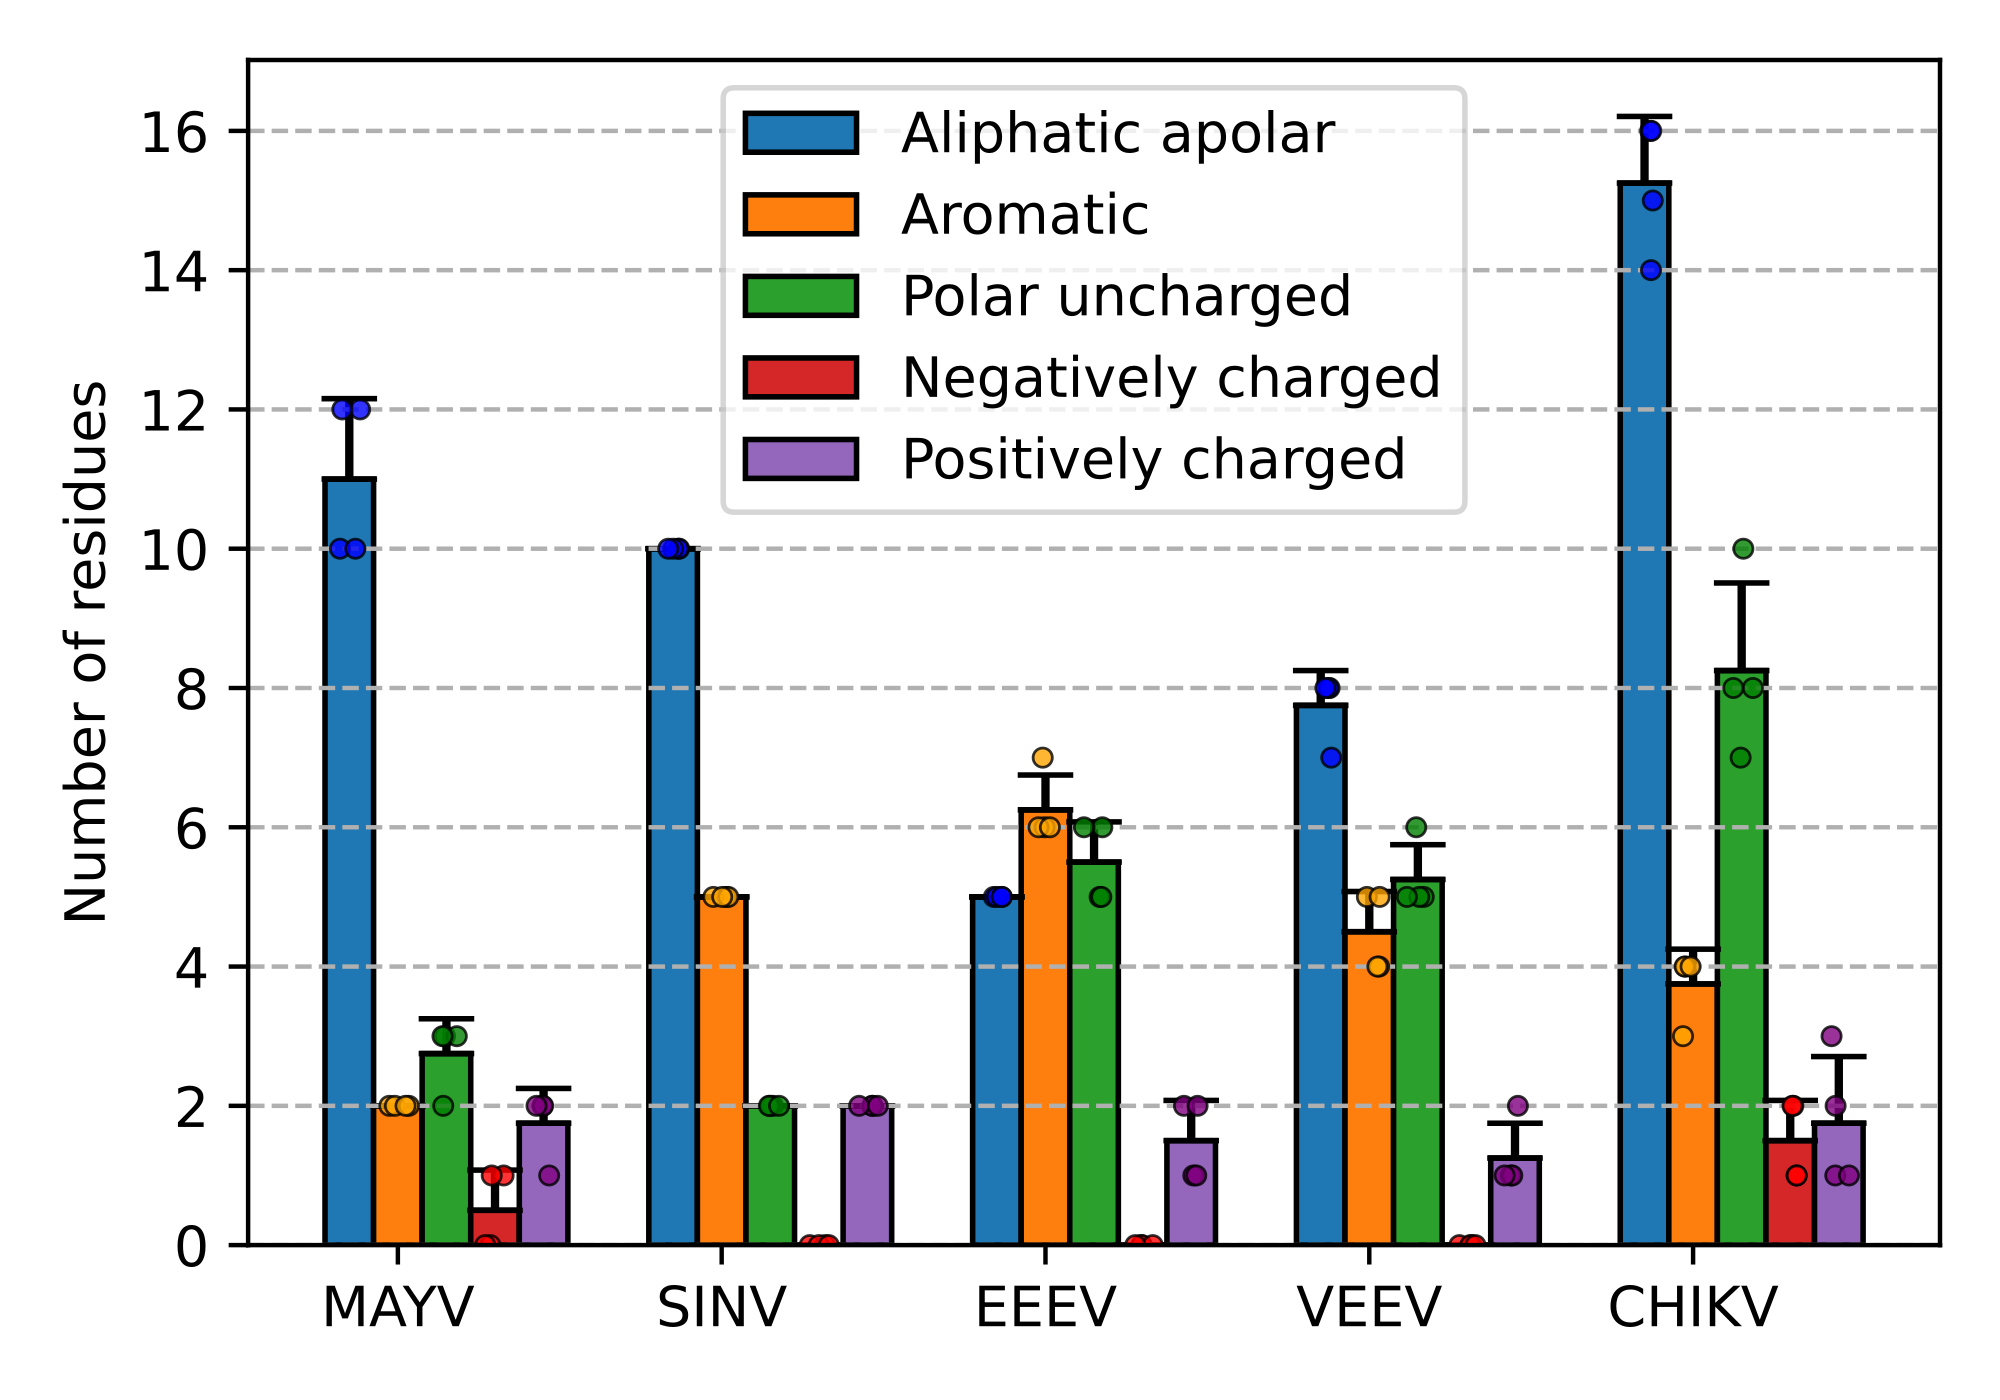
\includegraphics[scale=0.5]{images/mayv-e1-e2-res-dist.png}
  \caption[Características estruturais extraídas da cavidade entre as hélices TM de E1 e E2 em MAYV e outros alphavírus]{\textbf{Características estruturais extraídas da cavidade entre as hélices TM de E1 e E2 em MAYV e outros alphavírus.} \textbf{(A)} Volume da cavidade estimado para os quatro heterodímeros E1-E2 (n = 4 estruturas independentes de heterodímeros) na unidade assimétrica. Um teste ANOVA unidirecional com comparação múltipla de Tukey foi utilizado para comparar o volume da cavidade do MAYV com outros alphavírus (* indica adj. p < 0,01 quando comparado aos alphavírus com MAYV). \textbf{(B)} Número de resíduos em cada um dos quatro heterodímeros E1-E2 (n = 4 estruturas independentes de heterodímeros) na unidade assimétrica, separados por classes. Um teste ANOVA unidirecional com comparação múltipla de Tukey foi utilizado para comparar o número de resíduos na classe alifática apolar com as outras classes na mesma espécie de alphavírus (* indica adj. p < 0,01 quando comparando a classe alifática apolar com as outras classes). Todos os dados são apresentados como valores médios +/- DP. Alifática apolar: ALA, VAL, ILE, LEU, GLY, PRO; Aromática: PHE, TYR, TRP; Polar não carregada: SER, THR, CYS, MET, ASN, GLN; Carregada negativamente: GLU, ASP; Carregada positivamente: ARG, LYS, HIS.}
  \label{fig:mayv-e1-e2-plots}
\end{figure}

Para compreender melhor o ambiente do bolsão e extrair suas características químicas, o bolsão completo do MAYV foi caracterizada usando o parKVFinder \cite{guerra2020} e comparado com os bolsões de outros alphavírus. Os ectodomínios de E1 e E2 do MAYV (PDB ID: 7KO8), SINDV (PDB ID: 6IMM), vírus da Encefalite Equina Oriental (EEEV; PDB ID: 6MX4), vírus da Encefalite Equina Venezuelana (VEEV; PDB ID: 3J0C) e Vírus Chikungunya (CHIKV; PDB ID: 6NK5) foram usados para detecção e caracterização do bolsão hidrofóbico. No MAYV, a cavidade entre os domínios E1 e E2 possui um volume de $\aproximadamente850 \mAA^3$ (Figura \ref{fig:mayv-e1-e2-plots}). Esse volume é bastante semelhante em SIND, EEEV e VEEV, mas em CHIKV, E1 e E2 estão mais distantes um do outro, o que cria um volume maior.

A natureza hidrofóbica do bolsão em alphavírus é claramente observada pelo mapeamento da superfície de hidrofobicidade (Figura \ref{fig:mayv-e1-e2-analysis}C) e pelo número de resíduos apolares que formam o núcleo da cavidade (Figura \ref{fig:mayv-e1-e2-plots}). A densidade do bolsão se estende até resíduos polares, como H362, T365 e T366 do domínio E2 na abertura posterior (Figura \ref{fig:mayv-e1-e2-plots}), indicando que a molécula pode ter uma natureza anfipática, como um ácido graxo. T365 e T366 têm uma posição estrutural conservada em outros alphavírus ou são substituídos por serina, um resíduo ainda mais polar. Na abertura posterior, outra histidina (H352 do E2) ajuda a fechar o bolsão. A maioria dos alphavírus, exceto o SINV, possui resíduos de histidina ocupando uma posição semelhante. Em conjunto, essas descobertas indicam que os alphavírus têm uma cavidade anfipática consistente formada entre os domínios E1 e E2 na membrana externa da bicamada lipídica. Caso o bolsão alphaviral seja ocupado por uma molécula, essa molécula seria quimicamente similar em diferentes alphavírus. O mapa de densidade do MAYV sugere que a densidade extra pode ser ocupada por um ácido graxo que pode aprimorar as interações entre E1 e E2. Portanto, o bolsão pode ser alvo para o desenvolvimento de compostos antivirais contra o MAYV e outros alphavírus, usando o desenho racional de fármacos.

Por outro lado, as proteínas nucleocapsídicas C dos alphavírus são compostas por dois subdomínios: um domínio N-terminal desordenado que se liga ao RNA viral, que não é observado no mapa de densidade do MAYV, e um domínio C-terminal estruturado que se liga às proteínas E2. A região N-terminal tem menor identidade entre os alphavírus e é relatada como específica do vírus \cite{ribeiro2021}.

O mapa de densidade do MAYV confirma a estrutura geralmente conservada da proteína C, formando dois subdomínios ricos em folhas beta separados por uma cavidade rasa ($\aproximadamente500 \mAA^3$, Figura \ref{fig:mayv-c-e2-plots}), na qual o domínio C-terminal da proteína E2 se liga não covalentemente. O fundo do bolsão é hidrofóbico, enquanto seu topo possui resíduos polares e carregados. A interface entre o capsídeo e a proteína E2 envolve o motivo de consenso TPY (resíduos T387, P398 and Y399), que é conservado dentro do gênero \textit{Alphavirus}. Curiosamente, pequenas moléculas propostas para inibir a interação entre o capsídeo e a proteína E2 contêm anéis heterocíclicos, o que reforça a relevância desse tipo de contato para a interação entre o capsídeo e a proteína E2 e destaca esse sítio como um potencial alvo de drogas.

\begin{figure}[t]
  \centerline{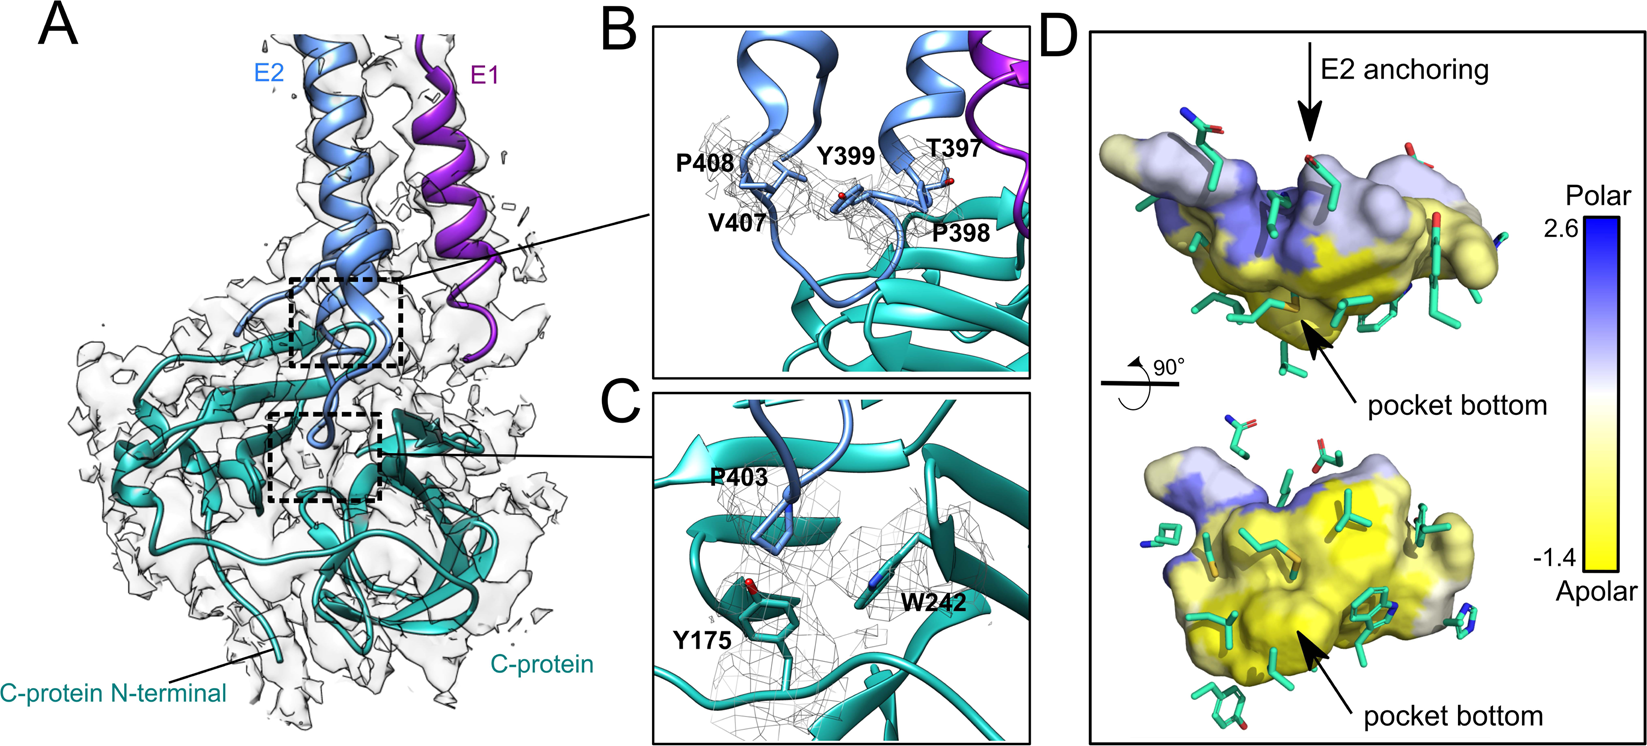
\includegraphics[scale=0.2]{images/mayv-c-e2-analysis.png}}
  \caption[Interação da cápside do MAYV com o domínio C-terminal da proteína E2]{\textbf{Interação da cápside do MAYV com o domínio C-terminal da proteína E2.} \textbf{(A)} Modelo atômico 3D do MAYV ajustado ao mapa de densidade obtido por criomicroscopia eletrônica. As proteínas C, E1 e E2 são representadas como desenhos em ciano, roxo e azul, respectivamente. \textbf{(B)} A interação do motivo TPY (resíduos T387, P398 e Y399) com a proteína C. \textbf{(C)} Os resíduos P403 e T402 da E2 e sua interação com os resíduos aromáticos Y175 e W242 na proteína C. O mapa de densidade do MAYV é mostrado em representação de malha. \textbf{(D)} Prospeção da cavidade na proteína C do MAYV, mostrando um ambiente hidrofóbico na parte inferior do bolso e um ambiente polar e carregado nas bordas externas da cavidade. A cavidade da proteína C que se liga ao domínio C-terminal da E2 é representada em superfície e colorida de acordo com a escala hidrofóbica de consenso de Eisenberg. Os resíduos da proteína C que cercam a cavidade são representados como \textit{sticks}.}
  \label{fig:mayv-c-e2-analysis}
\end{figure}

\begin{figure}[ht]
  \centering
    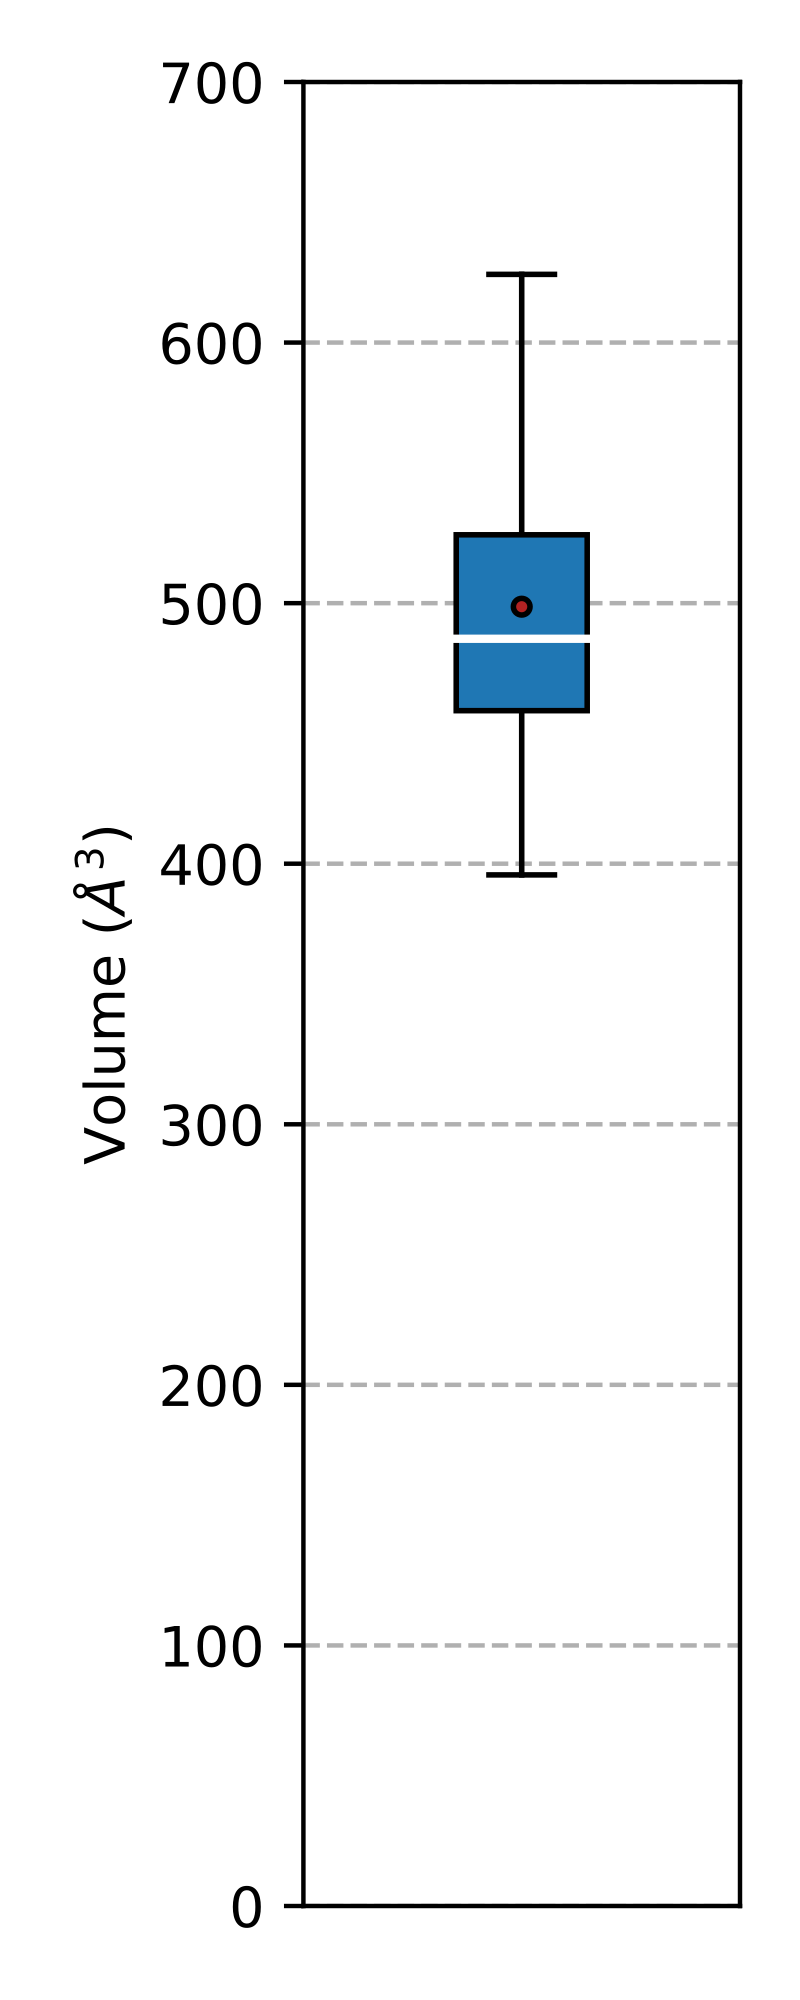
\includegraphics[scale=0.5]{images/mayv-c-e2-volume.png}
    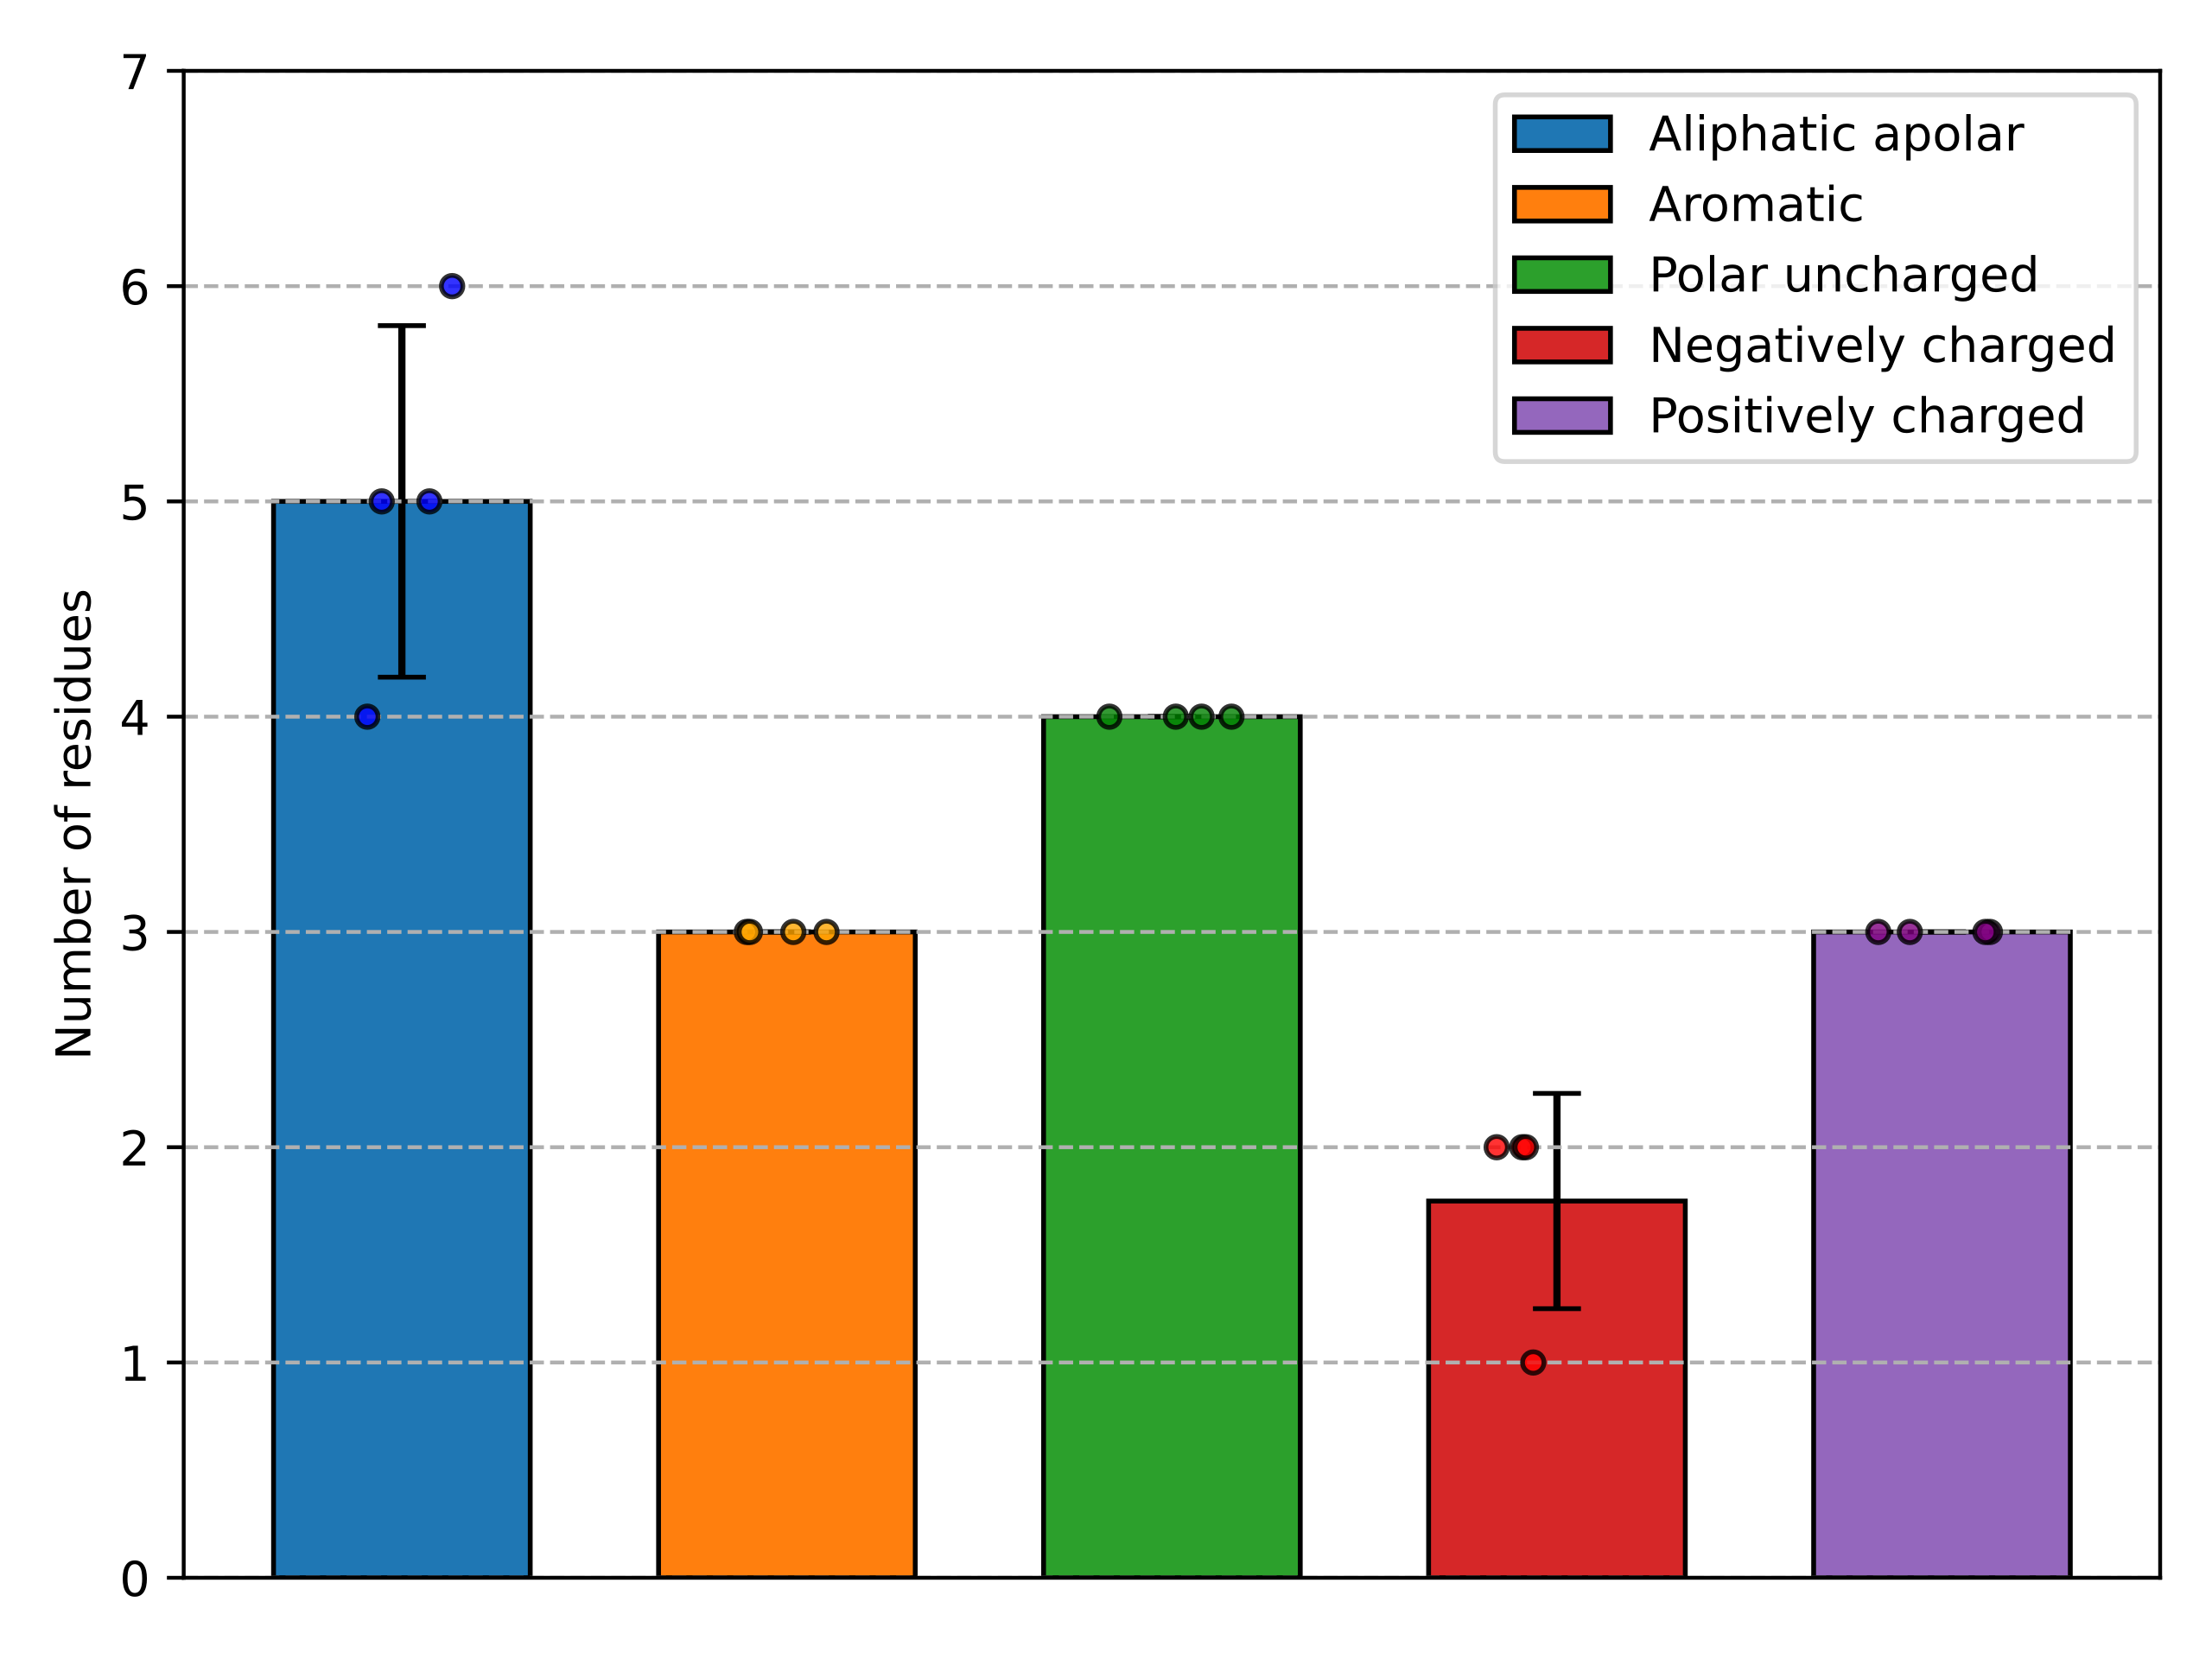
\includegraphics[scale=0.5]{images/mayv-c-e2-res-dist.png}
  \caption[Características estruturais extraídas da cavidade da proteína C que se liga ao domínio C-terminal da proteína E2]{\textbf{Características estruturais extraídas da cavidade da proteína C que se liga ao domínio C-terminal da proteína E2.} \textbf{(A)} Boxplot do volume da cavidade estimado para as quatro cápsides (n = 4 estruturas independentes de cápside) na unidade assimétrica. No boxplot, a caixa representa a amplitude interquartil (IQR) ($67,5 \mAA^3$), o 75º percentil (Q3) ($526,2 \mAA^3$) e o 25º percentil (Q1) ($458,7 \mAA^3$). A linha central indica a mediana ($486,3 \mAA^3$) e a média ($498,6 \mAA^3$) é indicada por um ponto. As "whiskers" com valor mínimo ($395,7 \mAA^3$) e valor máximo ($626,2 \mAA^3$) são determinadas usando Q1-1,5 x IQR e Q3+1,5 x IQR, respectivamente. \textbf{(B)} Número de resíduos em cada uma das quatro cápsides (n = 4 estruturas independentes de cápside) na unidade assimétrica separados por classes. O teste de análise de variância unidirecional (ANOVA) com teste de comparação múltipla de Tukey foi usado para comparar o número de resíduos na classe alifática apolar com as outras classes ($*$ indica $adj. p<0.01$ ao comparar a classe alifática apolar com as outras classes). Todos os dados são apresentados como valores médios +/- desvio padrão. Alifático apolar: ALA, VAL, ILE, LEU, GLY, PRO; Aromático: PHE, TYR, TRP; Polar não carregado: SER, THR, CYS, MET, ASN, GLN; Negativamente carregado: GLU, ASP; Positivamente carregado: ARG, LYS, HIS.}
  \label{fig:mayv-c-e2-plots}
\end{figure}

É importante ressaltar que os resultados completos e detalhes das análises estão disponíveis no artigo publicado no periódico \textit{Nature Communications} \cite{ribeiro2021}.

Apesar de termos obtido sucesso na aplicação do parKVFinder em simulações de dinâmica molecular \cite{guerra2020} e em um estudo comparativo \cite{ribeiro2021}, encontramos limitações ao utilizá-lo em aplicações automatizadas e comparações sistemáticas de sítios de ligação. Por essa razão, é necessário uma ferramenta mais apropriada para aplicações em ciência de dados, que ofereça um acesso simplificado a funções e estruturas de dados durante a análise. No entanto, é importante destacar que o parKVFinder ainda desempenha um papel importante na plataforma do KVFinder suite, principalmente na otimização dos parâmetros de detecção e caracterização, por meio do plugin gráfico do PyMOL (\textit{PyMOL2 parKVFinder Tools}), devido aos seus recursos visuais. Estes parâmetros otimizados podem ser posteriormente adotados em estudos automatizados e comparações sistemáticas de sítios de ligação. Por fim, o parKVFinder também continua sendo útil para análises estrutural e funcional focadas em uma única estrutura biomolecular.

% Extra information:
% - A total of 80 spikes, formed by trimers of E1–E2 heterodimers, protrude from the MAYV membrane. E1 and E2 proteins immerse into the lipid membrane through their transmembrane domain (TM) and the E2 C-terminal connects the spike to the capsid.
% - Given the relevance of E1–E2 ectodomains in host cell infection and induction of humoral immune responses, we compared the MAYV structure to CHIKV. These alphaviruses are closely related, cause similar diseases, and induce serological cross-reactivity that complicates diagnosis. 

% No entanto, a metodologia mostrou limitações para aplicações automatizadas e comparações sistemáticas de cavidades. Com isso, um pacote mais voltado para data science é desejável. Nesse cenário, pyKVFinder surgiu. 
% parKVFinder = bom para otimizar parametros de detecção pois tem visual cues devido ao plugin.
% pyKVFinder = bom para automatizar e comparar cavidades pois tem uma API e é mais fácil de usar em scripts.

\section{pyKVFinder}

No cenário de análise de cavidades de larga escala, os protocolos exigem rotinas e algoritmos eficientes construídos em estruturas de dados de fácil manipulação. As cavidades do parKVFinder, assim como em outros programas bem conhecidos, \eg, fpocket \cite{fpocket}, GHECOM \cite{ghecom} e POVME 3.0 \cite{povme}, são legíveis para humanos e facilmente exibidas em programas de visualização molecular, mas não são adequadamente estruturadas para serem diretamente incorporadas em protocolos automatizados ou aplicações de ciência de dados. Para atender essa necessidade, desenvolvemos o \textbf{Python-C Parallel KVFinder (pyKVFinder)} \cite{guerra2021}, um pacote Python de código aberto, licenciado sob GPL v3.0, para detectar e caracterizar cavidades em estruturas biomoleculares em protocolos automatizados e aplicações de ciência de dados. Posteriormente, o pyKVFinder foi publicado na BMC Bioinformatics \cite{guerra2021}, sendo lançado como \href{https://github.com/LBC-LNBio/pyKVFinder/tree/v0.2.5}{pyKVFinder v0.2.5}. Atualmente, o pyKVFinder está na versão \href{https://github.com/LBC-LNBio/pyKVFinder/tree/v0.6.2}{v0.6.2}. O código-fonte do pyKVFinder está disponível no seguinte repositório: \url{https://github.com/LBC-LNBio/pyKVFinder}.


O pyKVFinder aplica um \textit{Simplified Wrapper and Interface Generator} (SWIG; \url{https://www.swig.org}) para estender as operações de grade 3D, escritas em C, para a linguagem de programação de alto nível Python. No pyKVFinder, a biomolécula alvo é inserida em uma grade 3D regular, que é armazenada como uma matriz N-dimensional (\textit{ndarray}; \textit{N-dimensional array}) do pacote NumPy \cite{numpy}. Para detectar cavidades, a ferramenta utiliza o algoritmo de dupla sonda, conforme ilustrado na Figura \ref{fig:kvfinder-suite-schema}, que escaneia a estrutura biomolecular em busca de regiões de inacessibilidade (\ie, cavidades). Além das propriedades da cavidade, como volume, área e resíduos de interface, que são armazenados como dicionários de Python, o pyKVFinder também calcula a profundidade e a hidropatia das cavidades. Tanto os pontos da cavidade quanto essas propriedades espaciais e físico-químicas são armazenadas em \textit{ndarrays} e podem ser visualizadas usando pacotes de visualização molecular no Python (\eg, NGLView \cite{nglview}). Além disso, o pyKVFinder pode ser integrado a uma gama de pacotes e bibliotecas científicas (\eg, scikit-learn \cite{scikit-learn} e SciPy \cite{scipy}) para cálculos matemáticos, análise estatística e visualização tridimensional, usando interfaces interativas (\eg, \textit{IPython, Jupyter} e \textit{JupyterLab notebooks}). Desta forma, o pyKVFinder facilita complexas análises de dados bioestruturais com protocolos e algoritmos dentro do ecossistema Python, além de servir como bloco de construção para novas aplicações em ciência de dados, desenho racional de fármacos e descoberta de medicamentos. Assim, o pyKVFinder fornece uma maneira versátil de detectar e caracterizar cavidades biomoleculares e integrar essas informações em protocolos automatizados e aplicações de ciência de dados.

O desempenho computacional do pyKVFinder também foi avaliado no kv1000 \cite{guerra2020}, apresentando um tempo de execução consideravelmente menor que o parKVFinder, em média 31\% mais rápido. Mesmo ao adicionar as novas caracterizações disponíveis, profundidade e hidropatia, o desempenho do pyKVFinder foi reduzido em apenas 5\% (para profundidade) e 4\% (para hidropatia) em média, independentemente do número de \textit{threads} utilizados (Figura \ref{fig:pykvfinder-parkvfinder-kv1000-comparison}). A principal razão para o ganho de desempenho é a possibilidade adicional de paralelizar as rotinas, ou seja, a inserção de átomos na grade 3D na função de detecção (\ie, \textit{pyKVFinder.detect}), baseada em \textit{ndarrays}. A maior melhoria foi observada em proteínas com mais de 2000 átomos, alcançando uma velocidade $\aproximadamente4,3$ vezes maior em proteínas com 11000 átomos, o que beneficia o crescente número de estruturas de alta ordem resolvidas atualmente. Para proteínas muito pequenas ($\less2000$ átomos), que representam uma porção menor das estruturas disponíveis, o ganho de desempenho do pyKVFinder não foi significativo ou até menor do que o do parKVFinder, principalmente devido à leitura em Python do arquivo PDB ou XYZ do alvo (Figura \ref{fig:pykvfinder-speedup}). Portanto, usuários experientes que necessitam de rotinas de \textit{scripting} são encorajados a utilizar o pyKVFinder devido ao seu desempenho aprimorado, enquanto os iniciantes devem priorizar o parKVFinder devido ao seu comportamento monolítico e à simplicidade de instalação e execução. Além disso, a escalabilidade do pyKVFinder com o aumento do número de \textit{threads}, bem como o tempo absoluto para realizar a detecção das cavidades, são apresentados na Figura \ref{fig:pykvfinder-parkvfinder-kv1000-comparison}, seguindo o comportamento apresentado pelo parKVFinder \cite{guerra2020}.

\begin{figure}[ht]
    \centering
    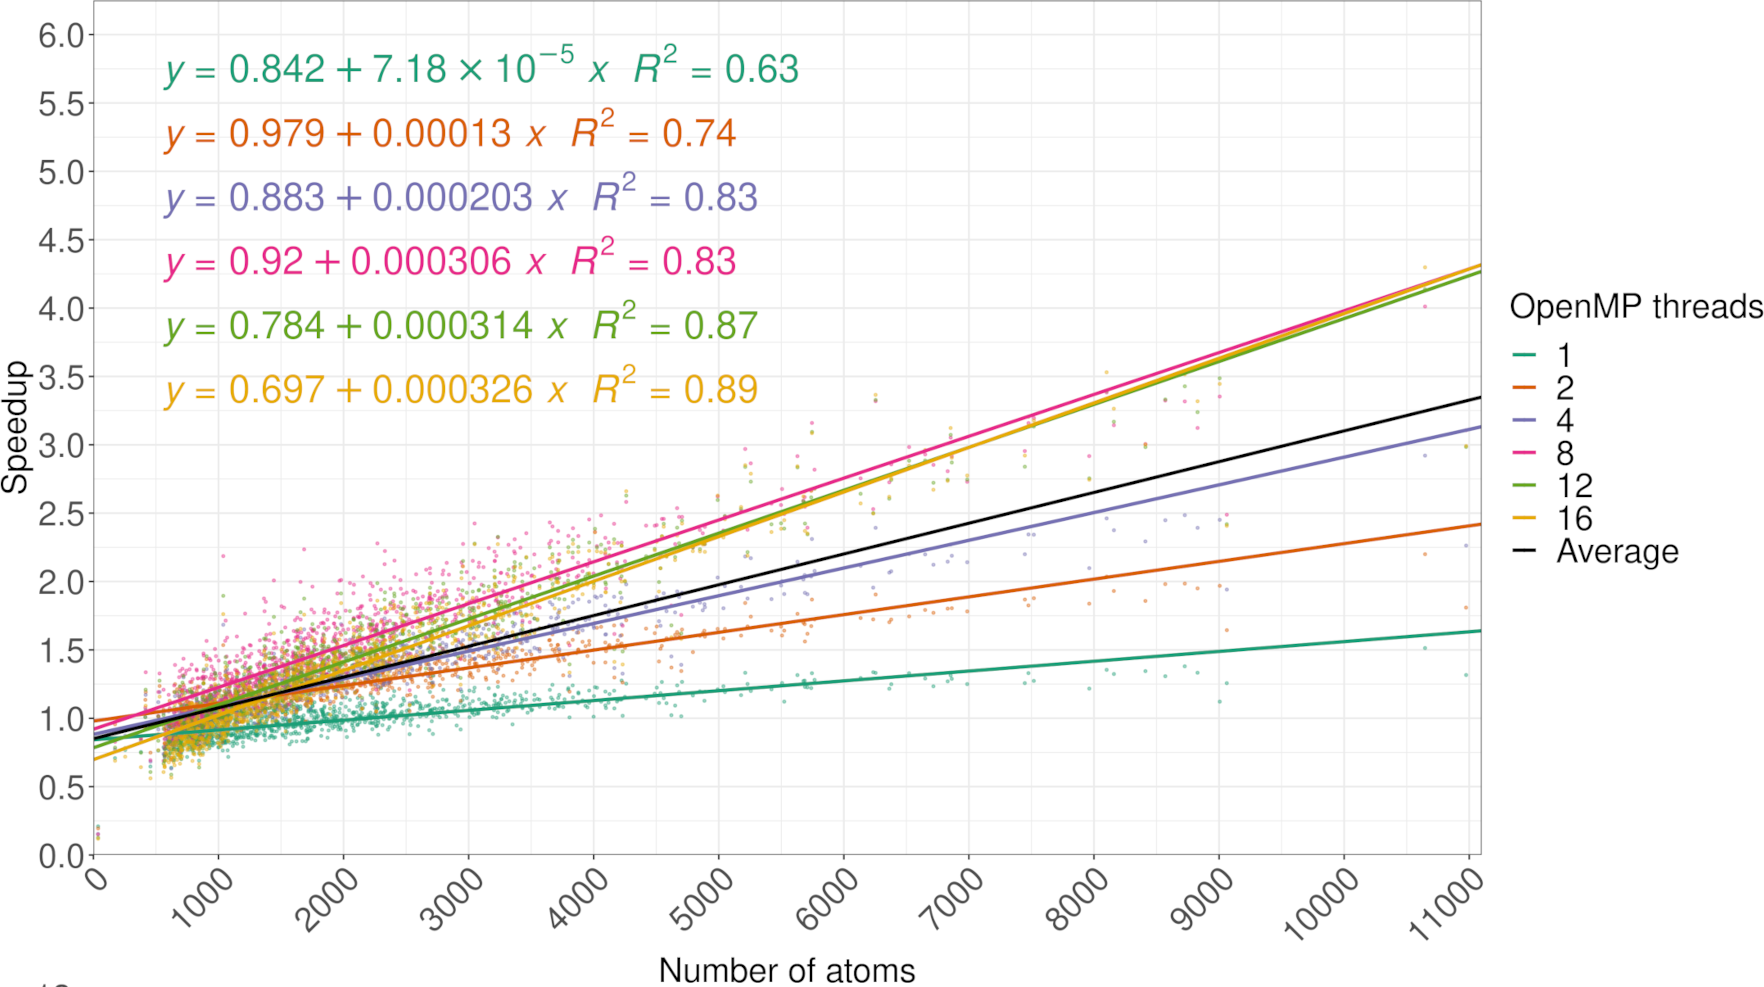
\includegraphics[scale=0.8]{images/pykvfinder-speedup.png}
    \caption[Ganho de velocidade do pyKVFinder comparado ao parKVFinder]{\textbf{Ganho de velocidade do pyKVFinder comparado ao parKVFinder.} O \textit{speedup} é a razão entre o tempo de execução do pyKVFinder e o tempo de execução do parKVFinder, aplicando o mesmo número de OpenMP \textit{threads}, para diferentes números de átomos.}
    \label{fig:pykvfinder-speedup}
\end{figure}

\subsection{Implementações de novas caracterizações}

Dentro do contexto do pyKVFinder, em colaboração com o Dr. György Szalóki (Laboratoire Hétérochimie Fondamentale et Appliquée - Université Toulouse III Paul Sabatier - França), o escopo do KVFinder suite foi expandido para uma nova classe de moléculas chamadas de gaiolas supramoleculares. Essas gaiolas são moléculas interconectadas que se unem de forma não-covalente, formando uma cavidade interna capaz de encapsular moléculas ou íons. A forma e o tamanho da cavidade são parâmetros importantes que podem ser facilmente determinados por algoritmos geométricos, auxiliando no desenho racional de gaiolas supramoleculares. Nesse contexto, também foram desenvolvidas novas caracterizações aplicáveis tanto para o contexto de gaiolas quanto para biomoléculas.

\subsubsection{Estimativa do volume molecular}

Para a modelagem da superfície molecular, desenvolvemos a classe \textit{Molecule} no pyKVFinder, que permite a modelagem das superfícies moleculares, conforme ilustrado na Figura \ref{fig:surface-representation}, e estimativa do volume molecular, como apresentado na Figura \ref{fig:molecular-modeling}. Nessa abordagem, as moléculas são inseridas em uma grade 3D regular, levando em consideração os raios de vdW de cada um dos átomos da molécula. Os usuários tem a flexibilidade de definir esses raios por meio de um arquivo de configuração (\textit{\href{https://github.com/LBC-LNBio/pyKVFinder/blob/master/pyKVFinder/data/vdw.dat}{vdw.dat}}), assim como a representação de superfície escolhida. Na grade 3D, cada voxel corresponde a um ponto de molécula (0) ou de solvente (1). Portanto, o volume de van der Waals da molécula é estimado somando-se os voxels rotulados como molécula na grade 3D. Essa funcionalidade de estimativa do volume molecular está disponível no pyKVFinder a partir da versão \href{https://github.com/LBC-LNBio/pyKVFinder/tree/v0.5.1}{v0.5.1}. A implementação desses recursos de modelagem e caracterização de moléculas foi detalhada e aplicadas em um artigo publicado no periódico \textit{Journal of Chemical Information and Modeling} \cite{guerra2023B}.

\begin{figure}[ht]
  \centering
  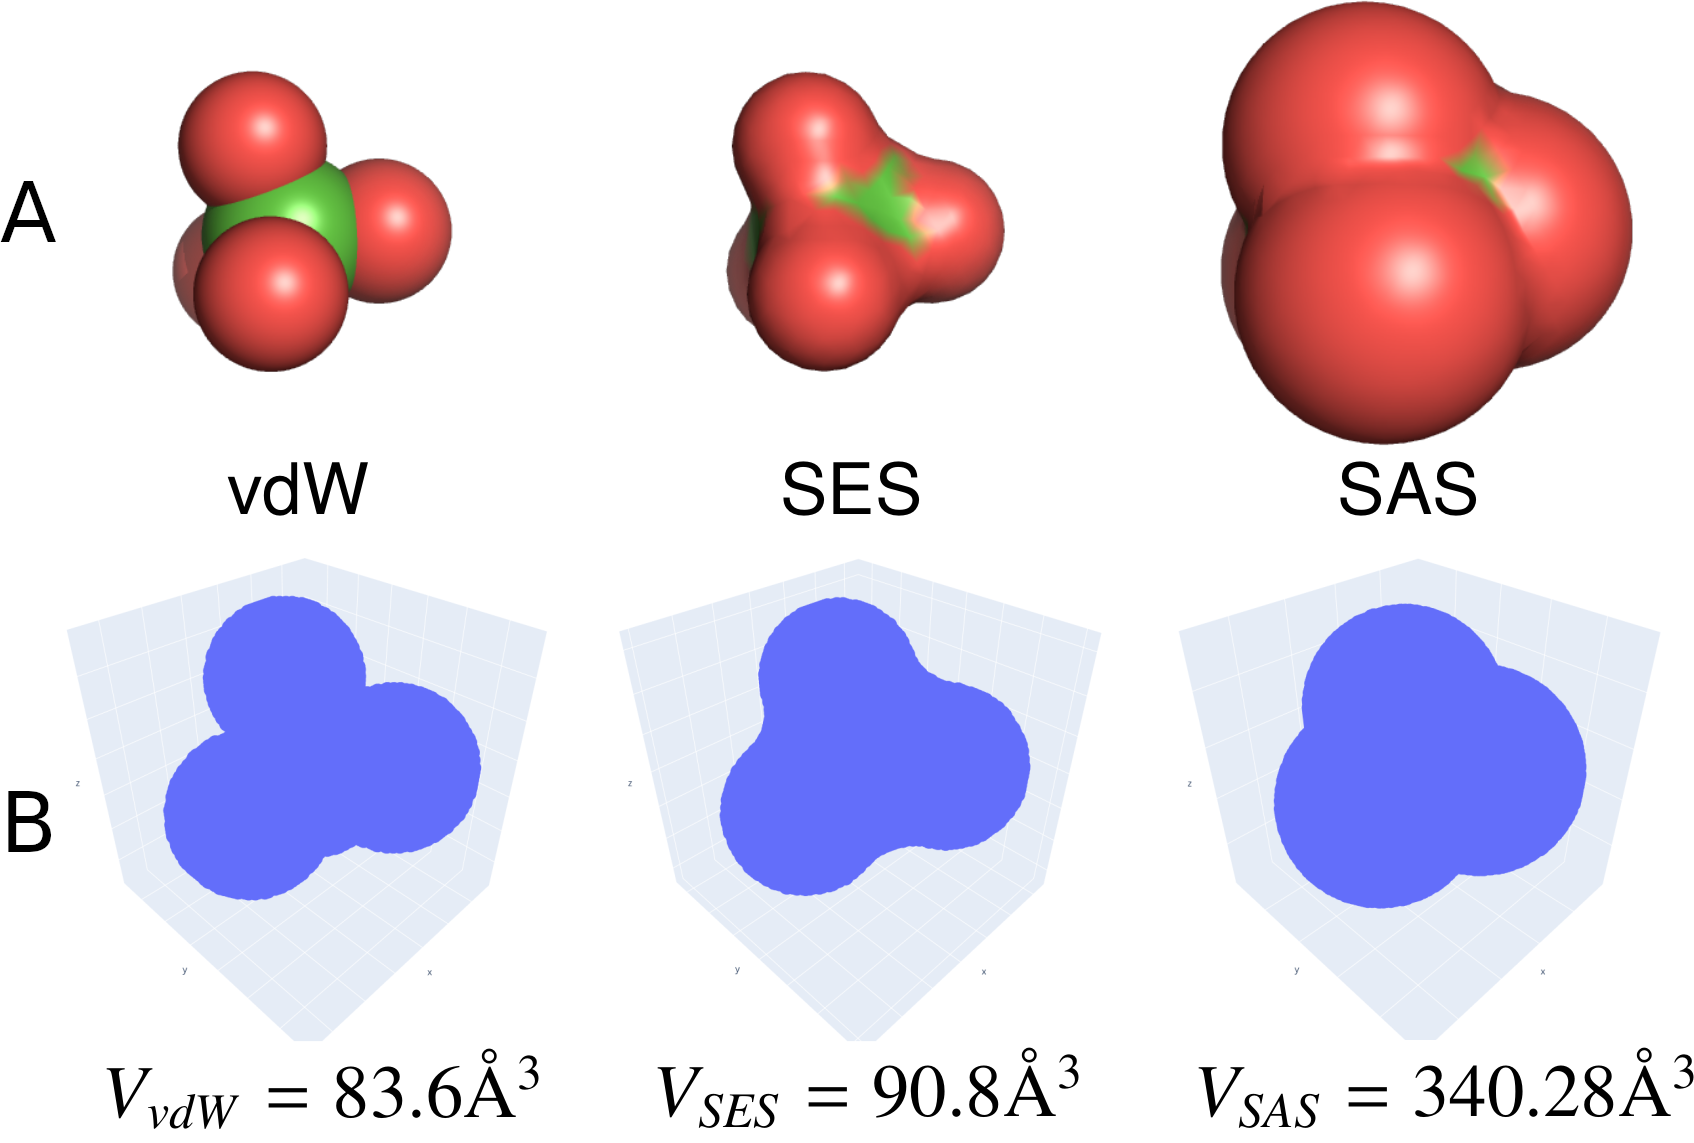
\includegraphics[scale=1.5]{images/molecular-modeling.png}
  \caption[Modelagem e estimativa de volume molecular do perclorato ($ClO_4$)]{\textbf{Modelagem e estimativa de volume molecular do perclorato ($ClO_4$).} \textbf{(A)} Superfície molecular de vdW (quadro esquerdo), SES (quadro central) e SAS (quadro direito) no visualizador molecular PyMOL. \textbf{(B)} Modelagem e estimativa do volume molecular de vdW (quadro esquerdo), SES (quadro central) e SAS (quadro direito) pelo pyKVFinder.}
  \label{fig:molecular-modeling}
\end{figure}

\subsubsection{Caracterização de aberturas}

A compreensão das características das gaiolas supramoleculares, como volume (Figura \ref{fig:cage-characterization}A) e abertura (Figura \ref{fig:cage-characterization}B), que impulsionam o encapsulamento de intermediários reativos é fundamental para o desenho racional de novas gaiolas supramoleculares com propriedades catalíticas aprimoradas. Nesse sentido, desenvolvemos uma caracterização de abertura utilizando o pyKVFinder, que permite a identificação das aberturas, a determinação da área dessas aberturas e a maior sonda esférica (\ie, átomo) que pode passar por cada abertura, conforme ilustrado na Figura \ref{fig:cage-characterization}. 

\begin{figure}[htb]
  \centering
  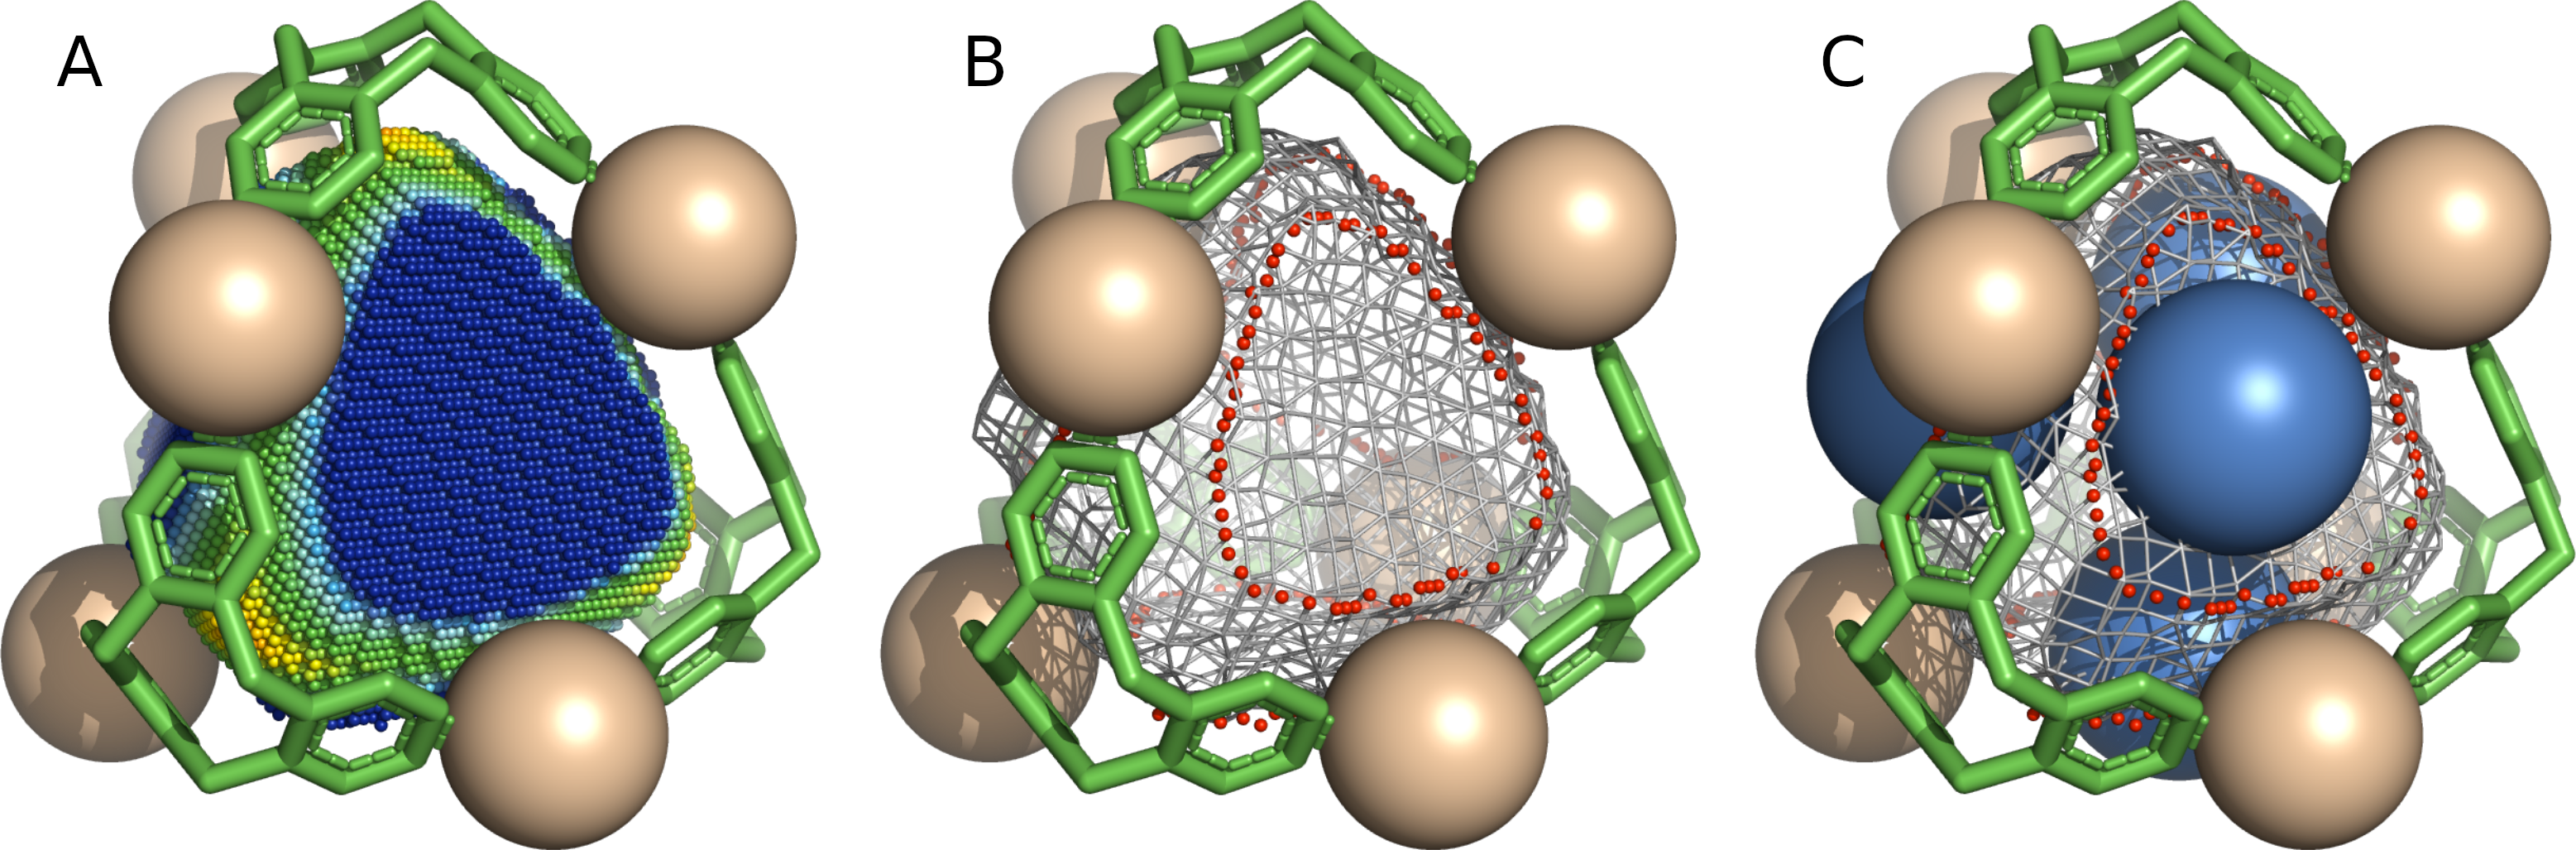
\includegraphics[scale=1.2]{images/cage-characterization.png}
  \caption[Caracterizações de gaiolas supramoleculares]{\textbf{Caracterizações de gaiolas supramoleculares.} \textbf{(A)} Volume e profundidade. Os pontos são coloridos de acordo a profundidade, sendo azul para menor profundidade e vermelho para maior profundidade. \textbf{(B)} Abertura (pontos vermelhos) e área da abertura. \textbf{(C)} Maior sonda esférica (esfera azul) acessível à cavidade da gaiola.}
  \label{fig:cage-characterization}
\end{figure}

% Melhorar descrição dos filtros espaciais

O sistema de dupla sonda utiliza identificadores inteiros para os pontos de cavidade (1), pontos de biomolécula (0) e pontos de meio (-1). Após a agrupamento dos pontos de cavidade pelo algoritmo \textit{Depth-First Search} (DFS), os pontos de cavidade são marcados com valores >2, e os pontos de cavidades que não atingiram o volume de corte (parâmetro \textit{volume cutoff}) são mantidos com o valor 1. Nessa abordagem, os pontos de cavidade localizados a uma unidade de grade de um ponto de meio, seguindo a relação do elemento estruturante de \textit{rank} 3 e conectividade 1 (Figura \ref{fig:elementos-estruturantes}), são os pontos de fronteira cavidade-meio, que são marcados com o valor negativo do identificador numérico da cavidade correspondente, conforme descrito para o cálculo de profundidade \cite{guerra2019,guerra2021}. A partir desses pontos de fronteira, é calculada a área superficial utilizando o procedimento de estimativa de área da plataforma KVFinder suite \cite{guerra2019,guerra2020}, que é equivalente à área da abertura. Em seguida, os pontos de fronteira cavidade-meio localizados a uma unidade de grade de um ponto de biomolécula, seguindo a relação do elemento estruturante de \textit{rank} 3 e conectividade 1 (Figura \ref{fig:elementos-estruturantes}), são identificados como pontos de abertura. Nesse estágio, uma nova grade 3D é gerada para acumular os pontos de abertura, que são marcados com o valor 1, enquanto os demais pontos recebem o valor 0. Após o agrupamento dos pontos de abertura pelo algoritmo DFS, os pontos de abertura são marcados com valores >2 (Figura \ref{fig:cage-characterization}B), e aberturas com menos pontos do que um corte definido pelo usuário são marcadas com o valor 1. Por fim, para cada abertura identificada, é calculado o ponto médio e a maior esfera é determinada a partir desse ponto médio, definindo assim o maior átomo que pode passar por essa abertura (Figura \ref{fig:cage-characterization}C).

\subsection{Casos de estudo}

O pyKVFinder foi aplicado em dois casos de estudo publicados em periódicos científicos para investigar proteínas de interesse terapêutico. Essas análises exploraram as características de cavidades de proteínas homólogas ao domínio ADRP do SARS-CoV-2 e a dinâmica molecular do domínio ADRP do SARS-CoV-2 \cite{guerra2021}. A seguir, descreveremos cada um desses casos de estudo em detalhes.

\subsubsection{SARS-CoV-2 e proteínas homólogas}

Entre as 15 proteínas não estruturais (Nsps; \textit{Non-structural proteins}, em inglês), o novo coronavírus da Síndrome Respiratória Aguda Grave 2 (SARS-CoV-2; \textit{Severe acute respiratory syndrome coronavirus 2}, em inglês) codifica um grande multidomínio Nsp3. Uma de suas unidades é o domínio fosfatase de ADP-ribose (ADRP; também conhecido como macromodomínio, MacroD) \cite{michalska2020}. Ainda em investigação para determinar suas funções exatas no ciclo de vida do coronavírus, o domínio ADRP reconhece ADP-ribose 1'-fosfato e parece desempenhar um papel importante na virulência e na regulação da imunidade inata à infecção \cite{fehr2016,claverie2020}. Nesse sentido, esforços recentes têm sido feitos para caracterizar o sítio de ligação de substrato de ADP-ribose e avaliar esse local como um possível alvo de drogas antivirais.

Para demonstrar as funcionalidades e vantagens do pyKVFinder, detectamos e caracterizamos uma cavidade da proteína ADRP do SARS-CoV-2 que forma o sítio de ligação do substrato (Figura \ref{fig:conservation-analysis}). Para evidenciar como o pyKVFinder se beneficia do ecossistema de Python, desenvolvemos esse caso de estudo em um Jupyter notebook, executando o passo-a-passo das funções, disponível em \url{https://github.com/LBC-LNBio/pyKVFinder/blob/master/examples/conservation-analysis/conservation-analysis.ipynb}. Ao detectar a cavidade, primeiramente caracterizamos seu volume, área e resíduos de interface (Figura \ref{fig:conservation-analysis}A). Para visualizar a proteína e a cavidade de forma tridimensional não necessitamos do PyMOL, e podemos visualizá-los no próprio notebook através do pacote NGLView \cite{nglview}. Em seguida determinamos a composição dos resíduos que formam a cavidade e, além de visualizarmos esses resíduos, apresentamos suas frequências em um histograma (Figura \ref{fig:conservation-analysis}B), utilizando a pacote matplotlib \cite{matplotlib}.

\begin{figure}[h]
  \centering
  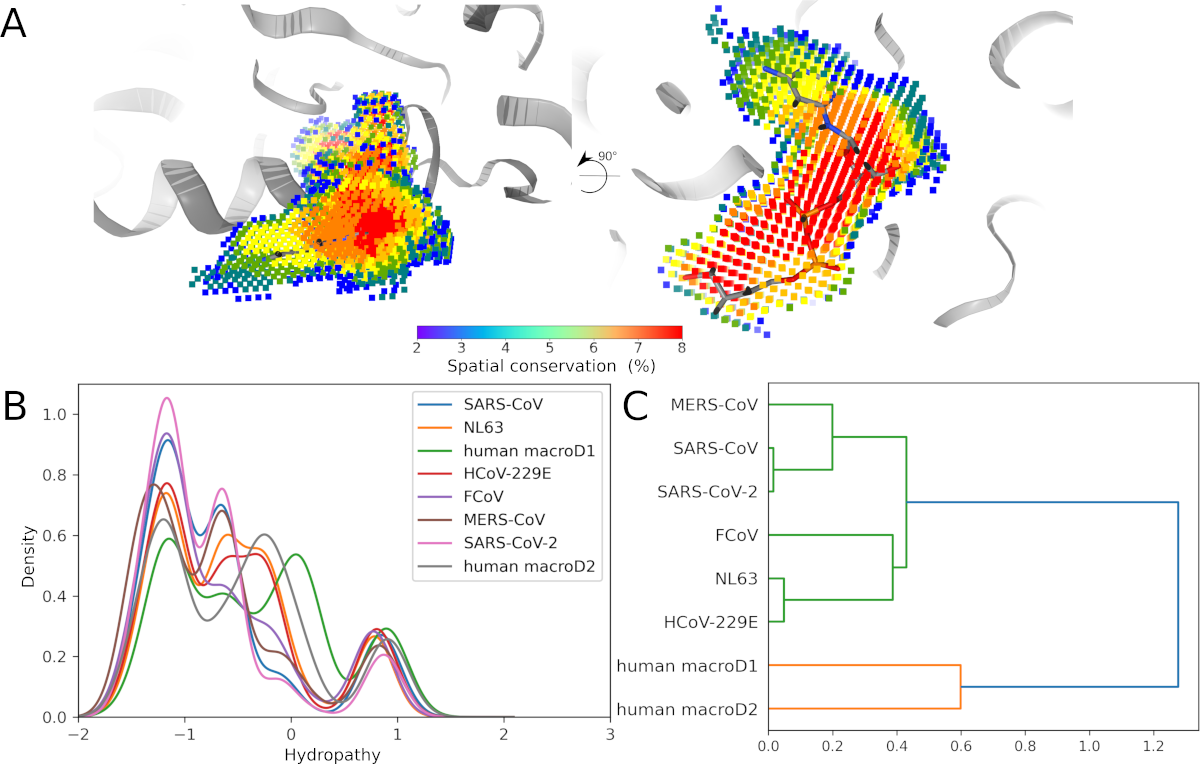
\includegraphics[scale=0.35]{images/adrp-sars-cov-2-conservation-analysis.png}
  \centerline{\scriptsize{\textbf{Fonte:} Adaptado de \cite{guerra2021}.}}
  \caption[Detecção e caracterização do sítio de ligação do substrato da ADRP do SARS-CoV-2 e sua comparação com coronavírus relacionados e proteínas humanas macroD1 e macroD2.]{\textbf{Detecção e caracterização do sítio de ligação do substrato da ADRP do SARS-CoV-2 e sua comparação com coronavírus relacionados e proteínas humanas macroD1 e macroD2.} \textbf{(A)} Caracterizações do sítio de ligação do substrato do domínio ADRP do SARS-CoV-2 (PDB ID: 6WEN). Esquerda: Cavidade detectada representada como uma superfície cinza e os resíduos ao redor dela como \textit{sticks} vermelhos. Centro: Cavidade colorida por profundidade. Direita: Cavidade colorida por hidropatia usando a escala de Eisenberg e Weiss. \textbf{(B)} Gráfico de barras das frequências de resíduos de interface. Esquerda: Aminoácidos. Direita: Classes de aminoácidos. \textbf{(C)} Análise de conservação do sítio de ligação do ADP-ribose no domínio ADRP do SARS-CoV-2 (PDB ID: 6WEN, cadeia A), SARS-CoV (PDB ID: 2ACF, cadeia B), MERS-CoV (PDB ID: 5HIH, cadeia A), NL63 (PDB ID: 2VRI, cadeia A), HCoV-229E (PDB ID: 3EJG, cadeia A), FCoV (PDB ID: 3ETI, cadeia B) e proteínas macrodomínio macroD1 (PDB ID: 2X47, cadeia A) e macroD2 (PDB ID: 6Y73, cadeia D) humanas. Os pontos de cavidade que foram detectados em pelo menos duas estruturas e os pontos são coloridos por porcentagem de conservação. \textbf{(D)} Perfil de hidropatia. \textbf{(E)} Dendrograma de agrupamento hierárquico da frequência de resíduos. A métrica de correlação de Pearson foi usada para avaliar a similaridade e o método completo foi escolhido como método de ligação. Todos os gráficos e imagens foram gerados em um Jupyter notebook. As imagens das estruturas tridimensionais foram geradas utilizando o pacote NGLView \cite{nglview} enquanto os gráficos foram construídos utilizando o pacote matplotlib \cite{matplotlib}.}
  \label{fig:conservation-analysis}
\end{figure}

Para compararmos a composição dessa cavidade com a de outros coronavírus ou proteínas humanas relacionadas, realizamos a mesma análise em outras 7 proteínas. Esses domínios de proteínas foram selecionados usando o Dali \cite{dali} e escolhendo homólogos na forma apo. As estruturas foram realinhadas usando o algoritmo MUSTANG \cite{mustang} do programa YASARA \cite{yasara}. 

% C: 

% D: 
Como o pyKVFinder utiliza dicionários em Python para armazenar os resíduos que formam a cavidade, podemos facilmente calcular a frequência desses resíduos. 

% E: 
Com essa informação, utilizamos o pacote SciPy \cite{scipy} para executar um método de agrupamento (\textit{clustering}, em inglês) hierárquico cujo resultado está representado no dendrograma da Figura \ref{fig:conservation-analysis}E. Nesse dendrograma, observamos o agrupamento das proteínas humanas relacionadas a proteína ADRP de coronavírus, e o agrupamento de coronavírus da mesma família, como o SARS-CoV-2, o SARS-CoV e o MERS.

Uma descrição detalhada dessa análise está disponível no artigo publicado no periódico \textit{BMC Bioinformatics} \cite{guerra2021}.

\subsubsection{Dinâmica molecular do domínio ADRP do SARS-CoV-2}

% Nesse contexto, o desempenho computacional do pyKVFinder foi avaliado em simulações de dinâmica molecular do domínio ADRP do SARS-CoV-2 (PDB ID: 6W02, chain B) sem seu ligante, a ADP-ribose, de 600 ns, extraindo quadros em intervalos regulares de 1 ns. Compared to its counterpart, parKVFinder,  pyKVFinder was 3.3 times faster in detecting ADRP binding site. The main reason for the performance gain is the additional possibility to parallelize routines, \ie, the insertion of atoms in the 3D grid in detect function, based on ndarrays. Hence, experienced users requiring scripting routines are encouraged to use pyKVFinder due to its improved performance, while newcomers should prioritize parKVFinder due to its simplicity of installation and execution. Further, the scalability of pyKVFinder, upon increasing number of threads, follows the same behavior presented by parKVFinder \cite{guerra2020}. Portanto, usuários experientes que necessitam de aplicações em larga escala são incentivados a utilizar o pyKVFinder devido ao seu desempenho aprimorado e flexibilidade, enquanto os iniciantes devem considerar o parKVFinder devido à sua simplicidade de instalação e execução.

Uma descrição detalhada dessa análise está disponível no artigo publicado no periódico \textit{BMC Bioinformatics} \cite{guerra2021}.

\section{KVFinder-web}

% Several web services have been proposed for the detection and/or characterization of binding sites in biomolecules. Amongst them, we could cite FpocketWeb (5), GHECOM (6), CaverWeb (7), CASTp (8), ConCavity (9), Depth (10), MoloVol (11) and 3DLigandSite (12).

O KVFinder-web é uma aplicação web de código aberto para detecção e caracterização de cavidades em qualquer tipo de estrutura biomolecular, que consiste em dois componentes independentes: um serviço web RESTful (KVFinder-web service) e uma interface web gráfica (KVFinder-web interface).  

O serviço web do KVFinder (KVFinder-web service) detecta e caracteriza espacialmente cavidades usando o parKVFinder, que implementa um método geométrico baseado em grade e esfera, para detectar cavidades em estruturas biomoleculares, com um sistema de dupla sonda [1, 2, 3]. O serviço web possui uma arquitetura Web-Fila-Trabalho (em inglês, Web-Queue-Worker), que processa as solicitações e respostas HTTP da interface web, gerencia os trabalhos e executa o parKVFinder nos trabalhos aceitos. O KVFinder-web service foi testado em um conjunto de dados de 1.000 domínios de proteínas únicos [1] com 6 conjuntos diferentes de parâmetros de detecção, mostrando consistência neste teste de alta demanda. 

A interface web do KVFinder (KVFinder-web interface; Figura 11), desenvolvida em R Shiny, disponibiliza as principais funcionalidades do KVFinder-web service, no qual os usuários podem carregar uma biomolécula alvo de um arquivo PDB ou pelo código PDB, personalizar parâmetros de detecção de cavidades e modos de execução, e baixar e visualizar resultados. A interface fornece uma maneira fácil e interativa de obter e visualizar os resultados da detecção de cavidades (Figura 12). Os volumes e áreas de cada cavidade são mostrados em uma tabela interativa, disponível para download no formato TOML. Um visualizador de biomoléculas, alimentado pelo motor NGL para R, exibe a estrutura biomolecular com suas cavidades, para download no formato PDB, e permite várias personalizações, por exemplo, realçar cavidades e exibir resíduos de interface ao redor das cavidades. A KVFinder-web interface está disponível para testes à equipe do CNPEM desde agosto de 2022 para projetos internos. 

Por fim, a disponibilização do KVFinder-web pretende ampliar o uso desta robusta ferramenta de detecção de cavidades na comunidade científica. Isso facilitará o processo de detecção e caracterização de cavidades, mesmo para usuários menos experientes, com impacto direto no desenvolvimento racional de medicamentos e no entendimento das estruturas das biomoléculas. 

\section{KVFinderMD}

% The protein-ligand and protein-protein interactions rely on the intrinsic dynamics of the target receptor, in which the classical lock and key model fails, and more recent binding models, e.g., induced-fit and conformation selection, thrive. Thus, molecular dynamics simulations are a useful tool to understand the underlying mechanisms of molecular recognition and, ultimately, the biomolecular function. In this scenario, we recently developed pyKVFinder, a Python package for detecting and characterizing biomolecular cavities in data science. Using it as a building block, we developed a new tool, called KVFinder for Molecular Dynamics analysis (KVFinderMD), to explore binding site dynamics in biomolecular structures of interest. Since the intrinsic biomolecule dynamics may change the shape and properties of the binding site over time, KVFinderMD can identify and characterize cavities in respect to volume, area, depth, hydropathy and interface residues, which are relevant properties to describe the molecular recognition process.

Em algumas circunstâncias, para a formação do complexo receptor-ligante, estes receptores utilizam sítios de ligação que não são facilmente identificados na forma não-ligada. Estas interações biomoleculares dependem da dinâmica intrínseca do receptor, nas quais o modelo clássico chave-fechadura falha, e modelos de ligação mais recentes, por exemplo, encaixe induzido e seleção de conformação, prosperam. Assim, as simulações de dinâmica molecular são uma ferramenta útil para entender os mecanismos de reconhecimento molecular e, em última análise, a função biomolecular. Nesse cenário, o LBC está desenvolvendo o KVFinderMD, usando o pyKVFinder [2] como bloco de construção, para explorar a dinâmica de sítios de ligação em estruturas biomoleculares de interesse farmacológico. Uma vez que a dinâmica intrínseca da biomolécula pode alterar a forma e as propriedades do sítio de ligação ao longo do tempo, o KVFinderMD pode identificar e caracterizar cavidades em relação ao volume, área, profundidade, hidropatia e resíduos de interface, que são propriedades relevantes para descrever o processo de reconhecimento molecular (Figura 14A). Além disso, também implementamos um algoritmo baseado em grafos, que considera distâncias carbono \textalpha, carbono \textbeta\space ou quaisquer átomos, para descrever topologicamente o sítio de ligação (Figura 14B).

Como provas de conceito, aplicamos o KVFinderMD em importantes alvos terapêuticos, como HIV-1 protease e ALDH1/2. Para HIV-1 protease, descrevemos com sucesso as alterações conformacionais que definem o sítio ativo, causadas principalmente pelos movimentos β-hairpins. Ainda, usando a representação gráfica de cavidades, exploramos algoritmos de agrupamento não supervisionados, como agrupamento hierárquico, com diferentes métricas de distância para agrupar com sucesso as cavidades ao longo da trajetória do receptor. No caso das ALDH1/2, exploramos as diferenças topológicas e volumétricas entre os sítios de ligação do substrato de ALDH1 e ALDH2, o que dita a preferência por aldeídos menores e maiores entre eles. Os resultados desse trabalho foram apresentados em detalhe no IV Congresso de Estudantes do CNPEM (IV CEC). 

\section{SERD}

O reconhecimento molecular depende diretamente da acessibilidade de um ligante ao sítios de ligação do seu respectivo receptor. Os resíduos expostos ao solvente de uma biomolécula alvo (receptor) compõe o conjunto de átomos acessíveis a possíveis ligantes. Nesse cenário, a identificação destes resíduos possibilita um estudo mais direcionado aos hotspots de interação de um receptor alvo, com aplicações principalmente no estudo de docking proteína-proteína. O programa SERD (https://github.com/jvsguerra/SERD) aproxima uma molécula de solvente a uma esfera, a qual escaneia a superfície do receptor alvo para identificar as regiões que são acessíveis a esta sonda esférica. Após a identificação destes resíduos, o programa os representa na forma de grafos pela biblioteca networkX (https://networkx.org/), formando arestas até uma distância limite entre carbonos \textalpha, carbonos-beta ou quaisquer átomos do resíduo e opcionalmente incluir essas distâncias como atributos das arestas desses grafos (Figura 13). 

\section{\textit{Benchmarking} das ferramentas disponíveis}

%%% Chapter 5

\chapter{Conclusões}

\begin{itemize}
  \item Comece explicando a importância dos sítios de ligação em biomoléculas e como eles afetam a função biológica das moléculas;
  \item Apresente os métodos experimentais e computacionais disponíveis para identificar e caracterizar sítios de ligação;
  \item Descreva brevemente os programas computacionais mais utilizados na área e suas principais características;
  \item Finalize apresentando o objetivo e a estrutura do seu trabalho.
 \end{itemize}

% As referências:
\bibliographystyle{abnt-num}
\bibliography{phdquali}


% Os anexos, se houver, vêm depois das referências:
\appendix

\chapter{Figuras suplementares}

\begin{figure}[htb]
  \centering
  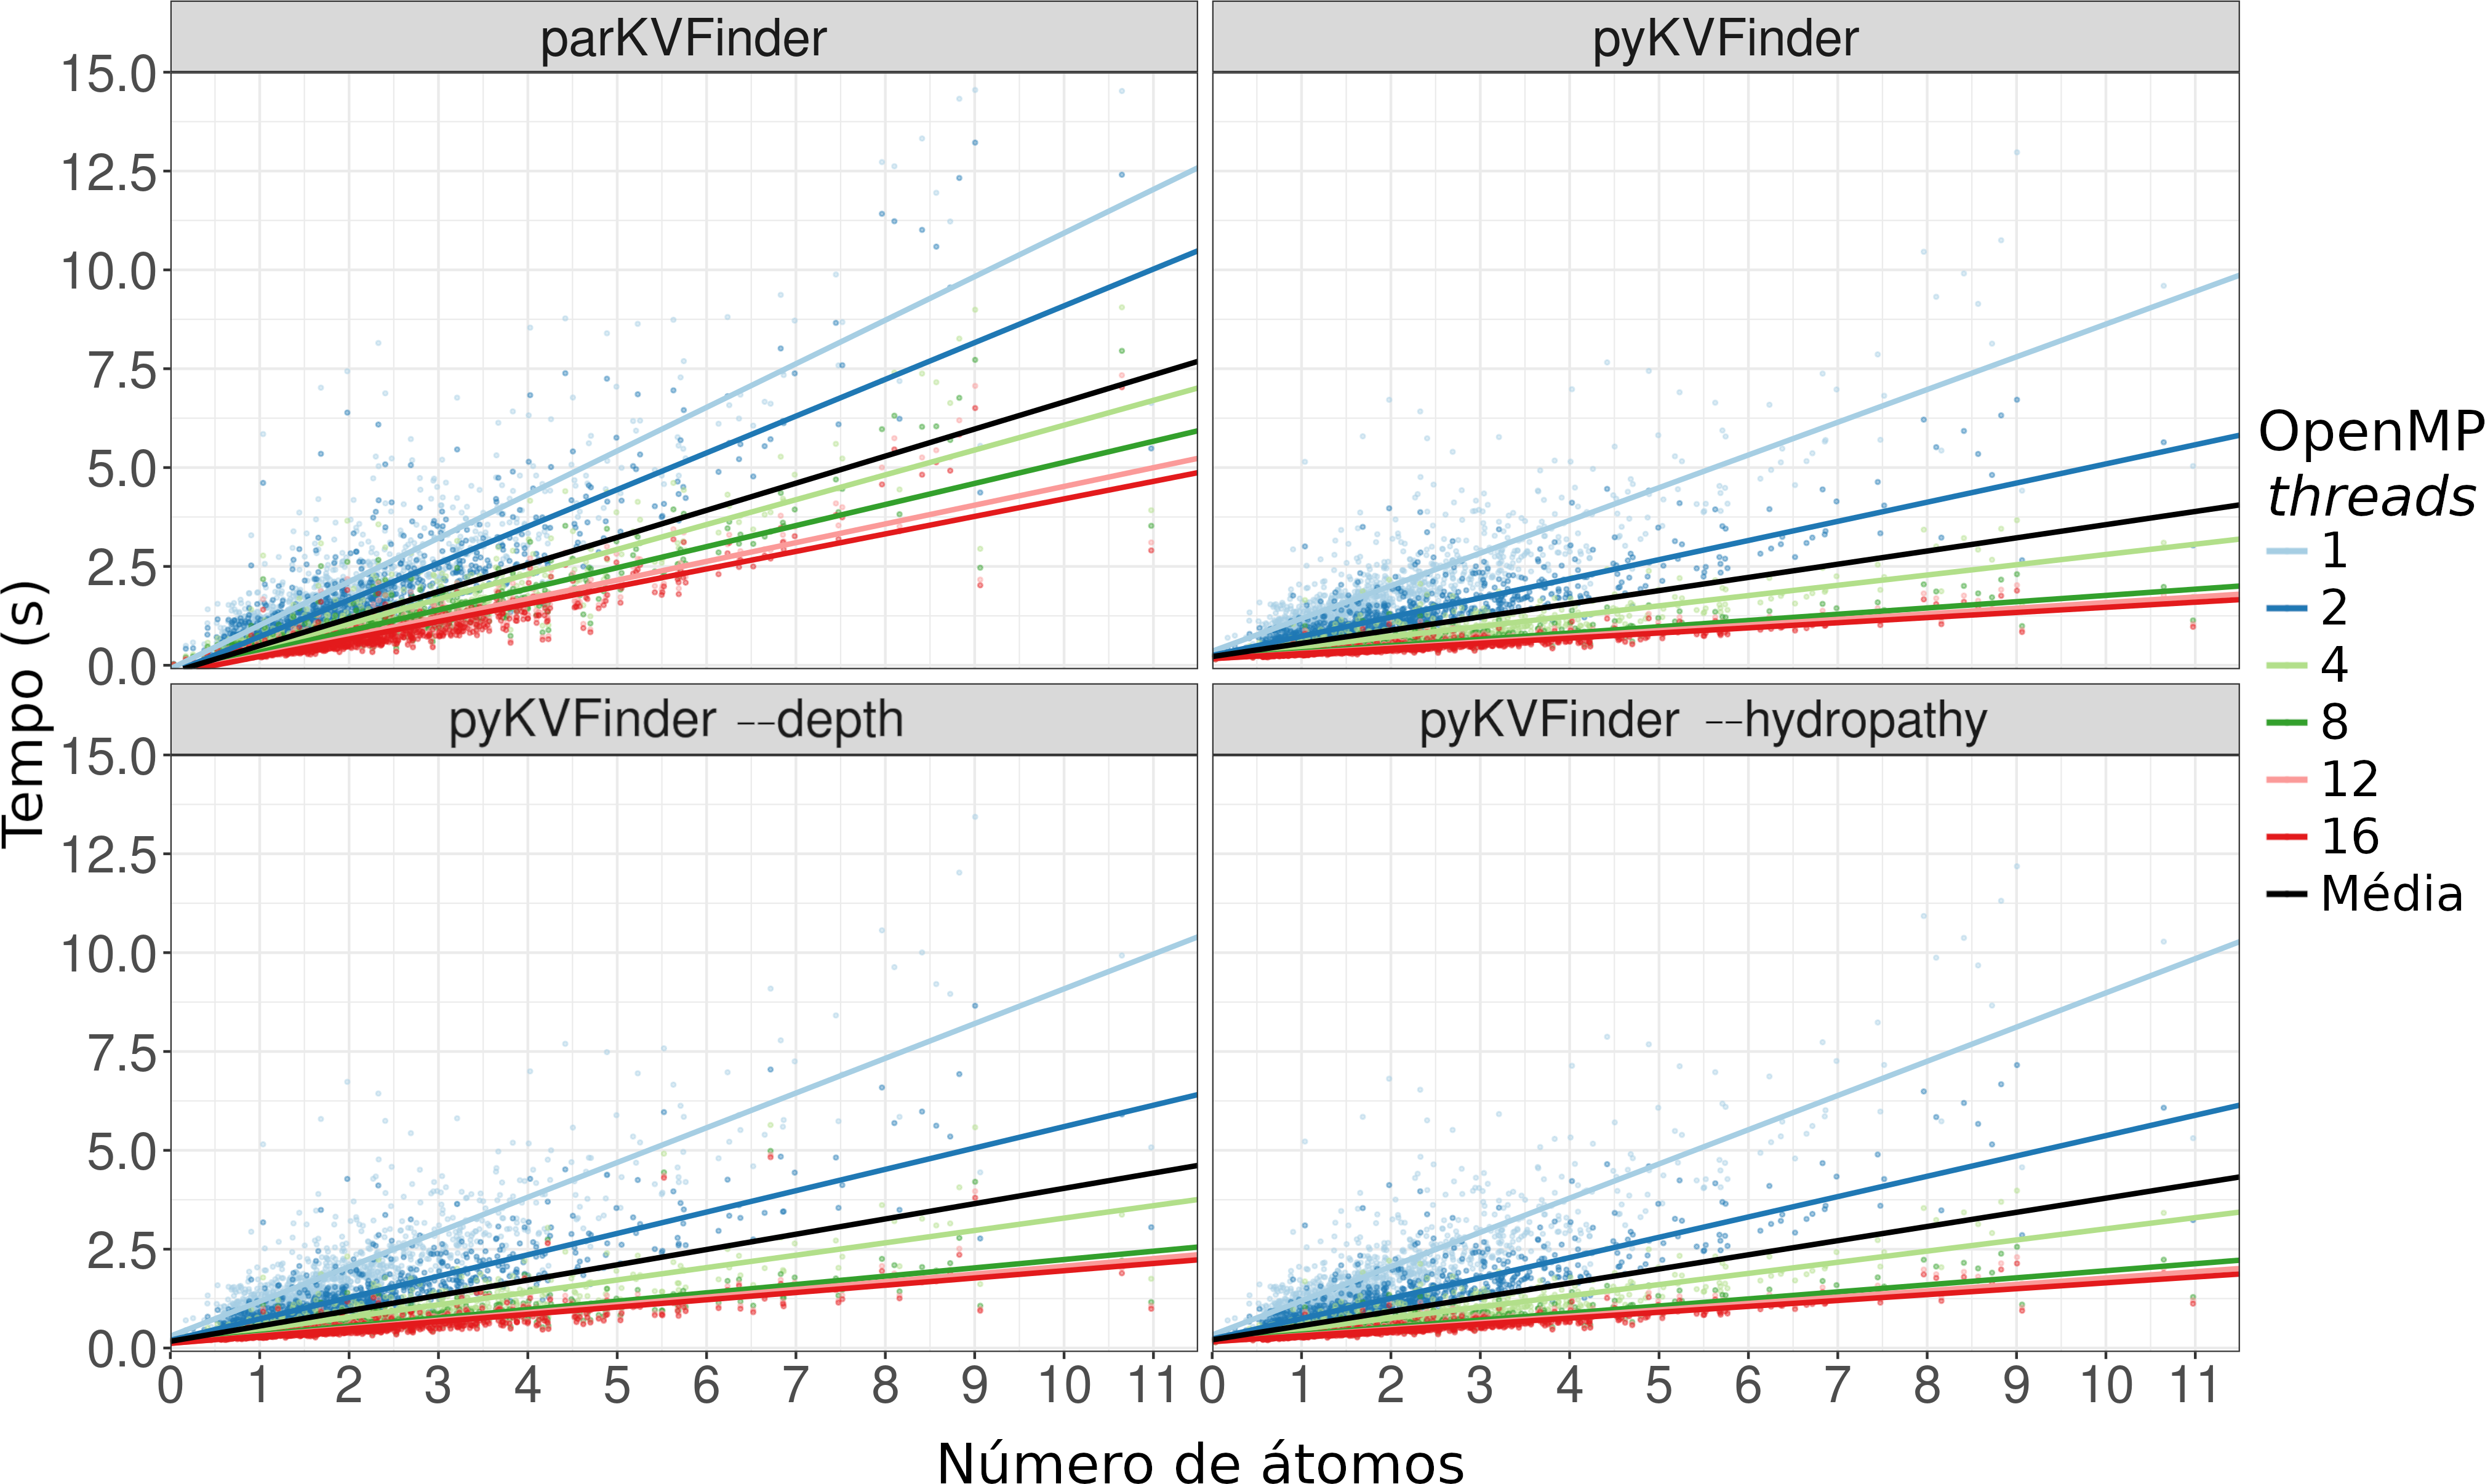
\includegraphics[scale=0.46]{images/pykvfinder-parkvfinder-kv1000-comparison.png}
  \caption[Ganho de velocidade do pyKVFinder comparado ao parKVFinder]{\textbf{Tempo computacional em função do número de átomos com diferentes números de \textit{threads} para o parKVFinder e o pyKVFinder.} Quadro superior esquerdo: parKVFinder. Quadro superior direito: pyKVFinder com caracterização padrão (volume, área e resíduos de interface). Quadro inferior esquerdo: pyKVFinder com caracterização padrão e de profundidade. Quadro inferior direito: pyKVFinder com caracterização padrão e de hidropatia}
  \label{fig:pykvfinder-parkvfinder-kv1000-comparison}
\end{figure}

\begin{figure}[htb]
  \centering
  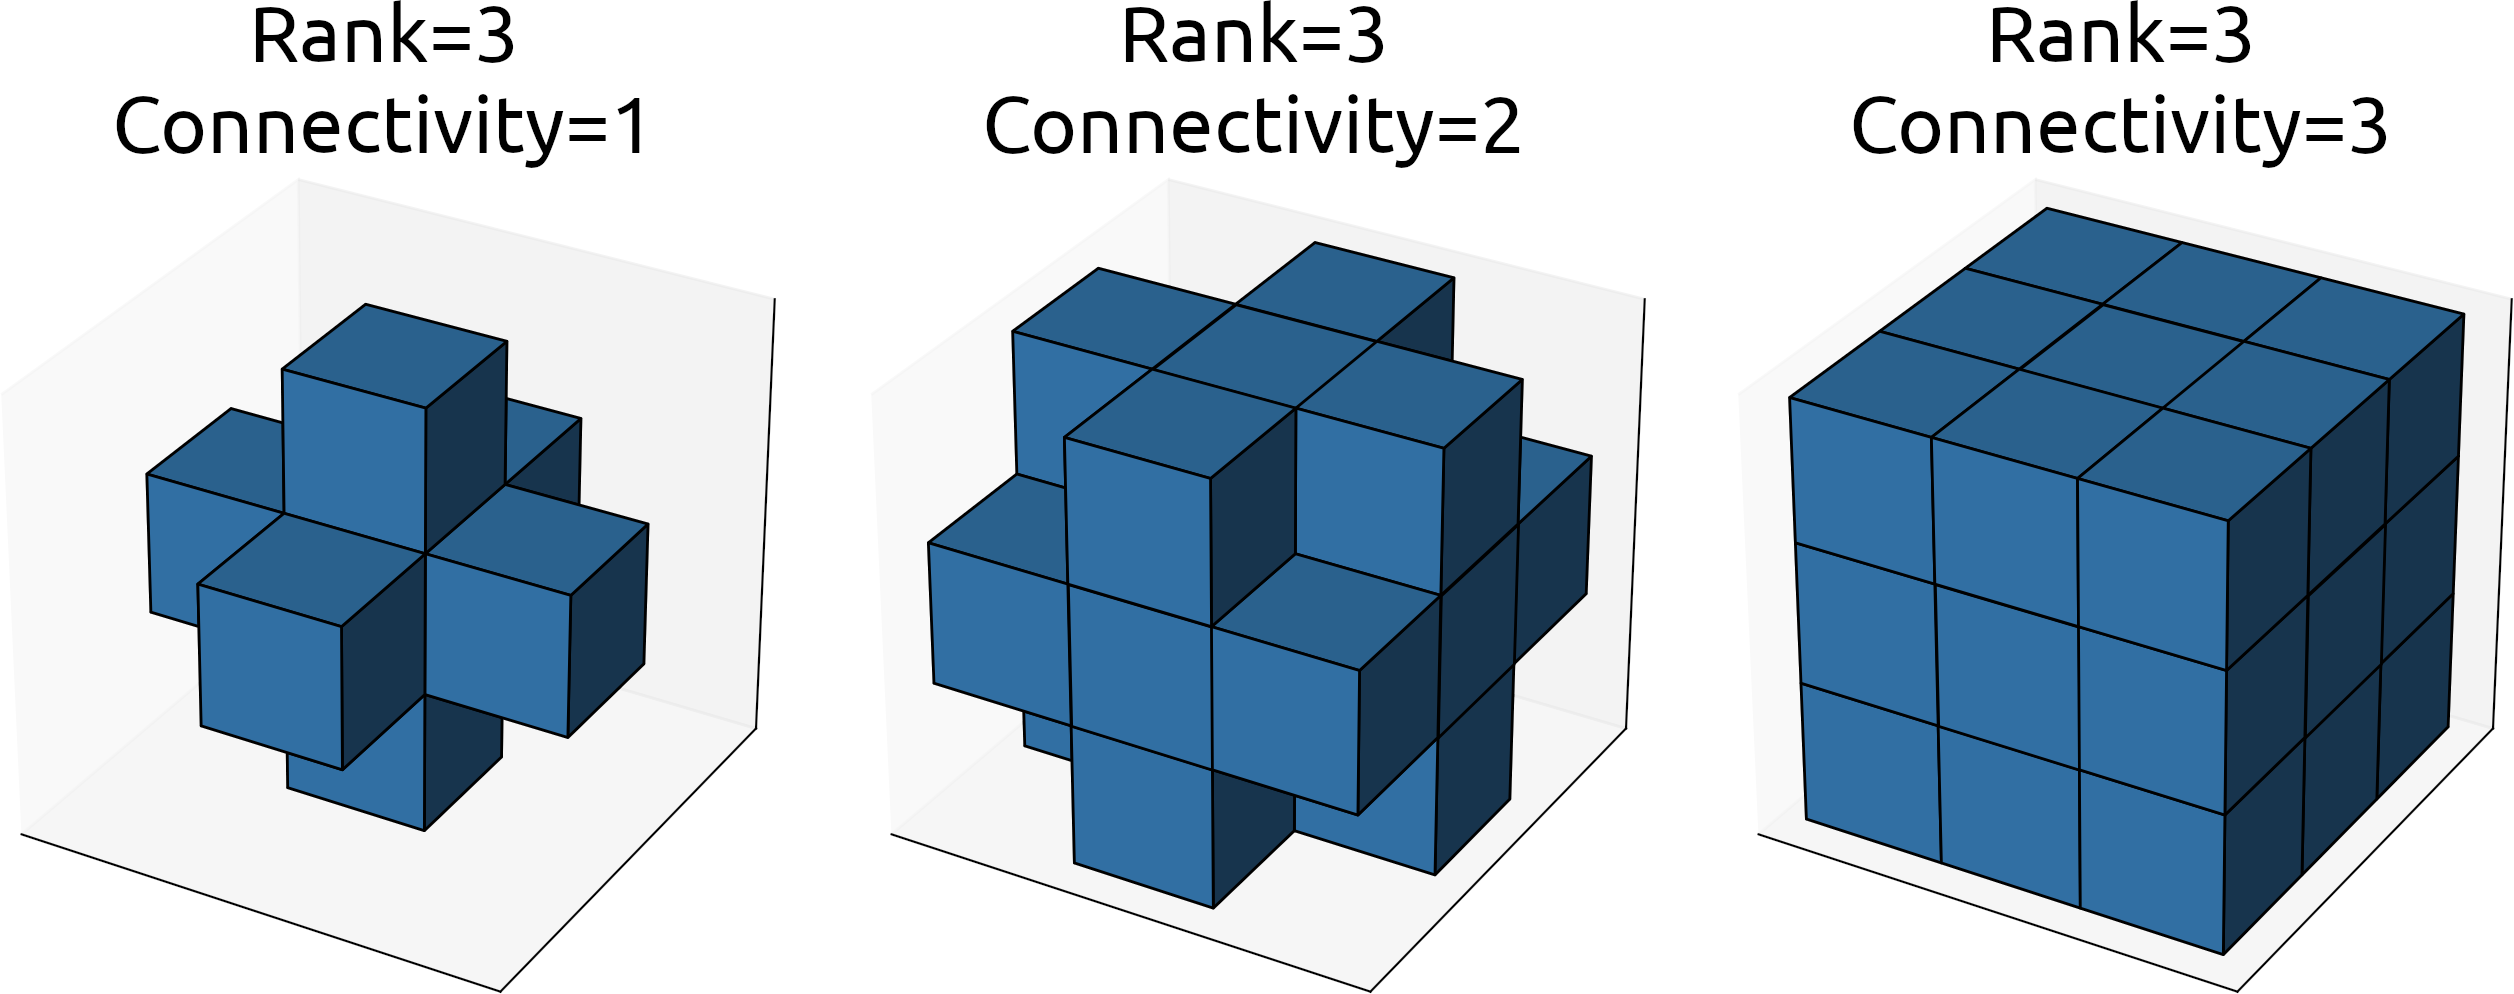
\includegraphics[scale=0.3]{images/3D-binary-structure.png}
  \centerline{\scriptsize{\textbf{Fonte:} Retirado de \url{https://docs.scipy.org/doc/scipy/tutorial/ndimage.html}}}
  \caption[Elementos estruturantes para filtros espaciais]{\textbf{Elementos estruturantes para filtros espaciais.}}
  \label{fig:elementos-estruturantes}
\end{figure}

\end{document}

% Table template

% \begin{table}
% \caption[Shorter table caption]{Table caption caption caption caption
%   caption caption caption caption caption caption caption caption caption
%   caption caption caption caption caption caption caption caption caption
%   caption caption.}
% \label{t:label0}
% \begin{center}
% \begin{tabular}{|c|c|}
% \hline
% a & b \\\hline
% c & d \\\hline
% \end{tabular}
% \end{center}
% \end{table}

% Figure template

% \begin{figure}
% \centerline{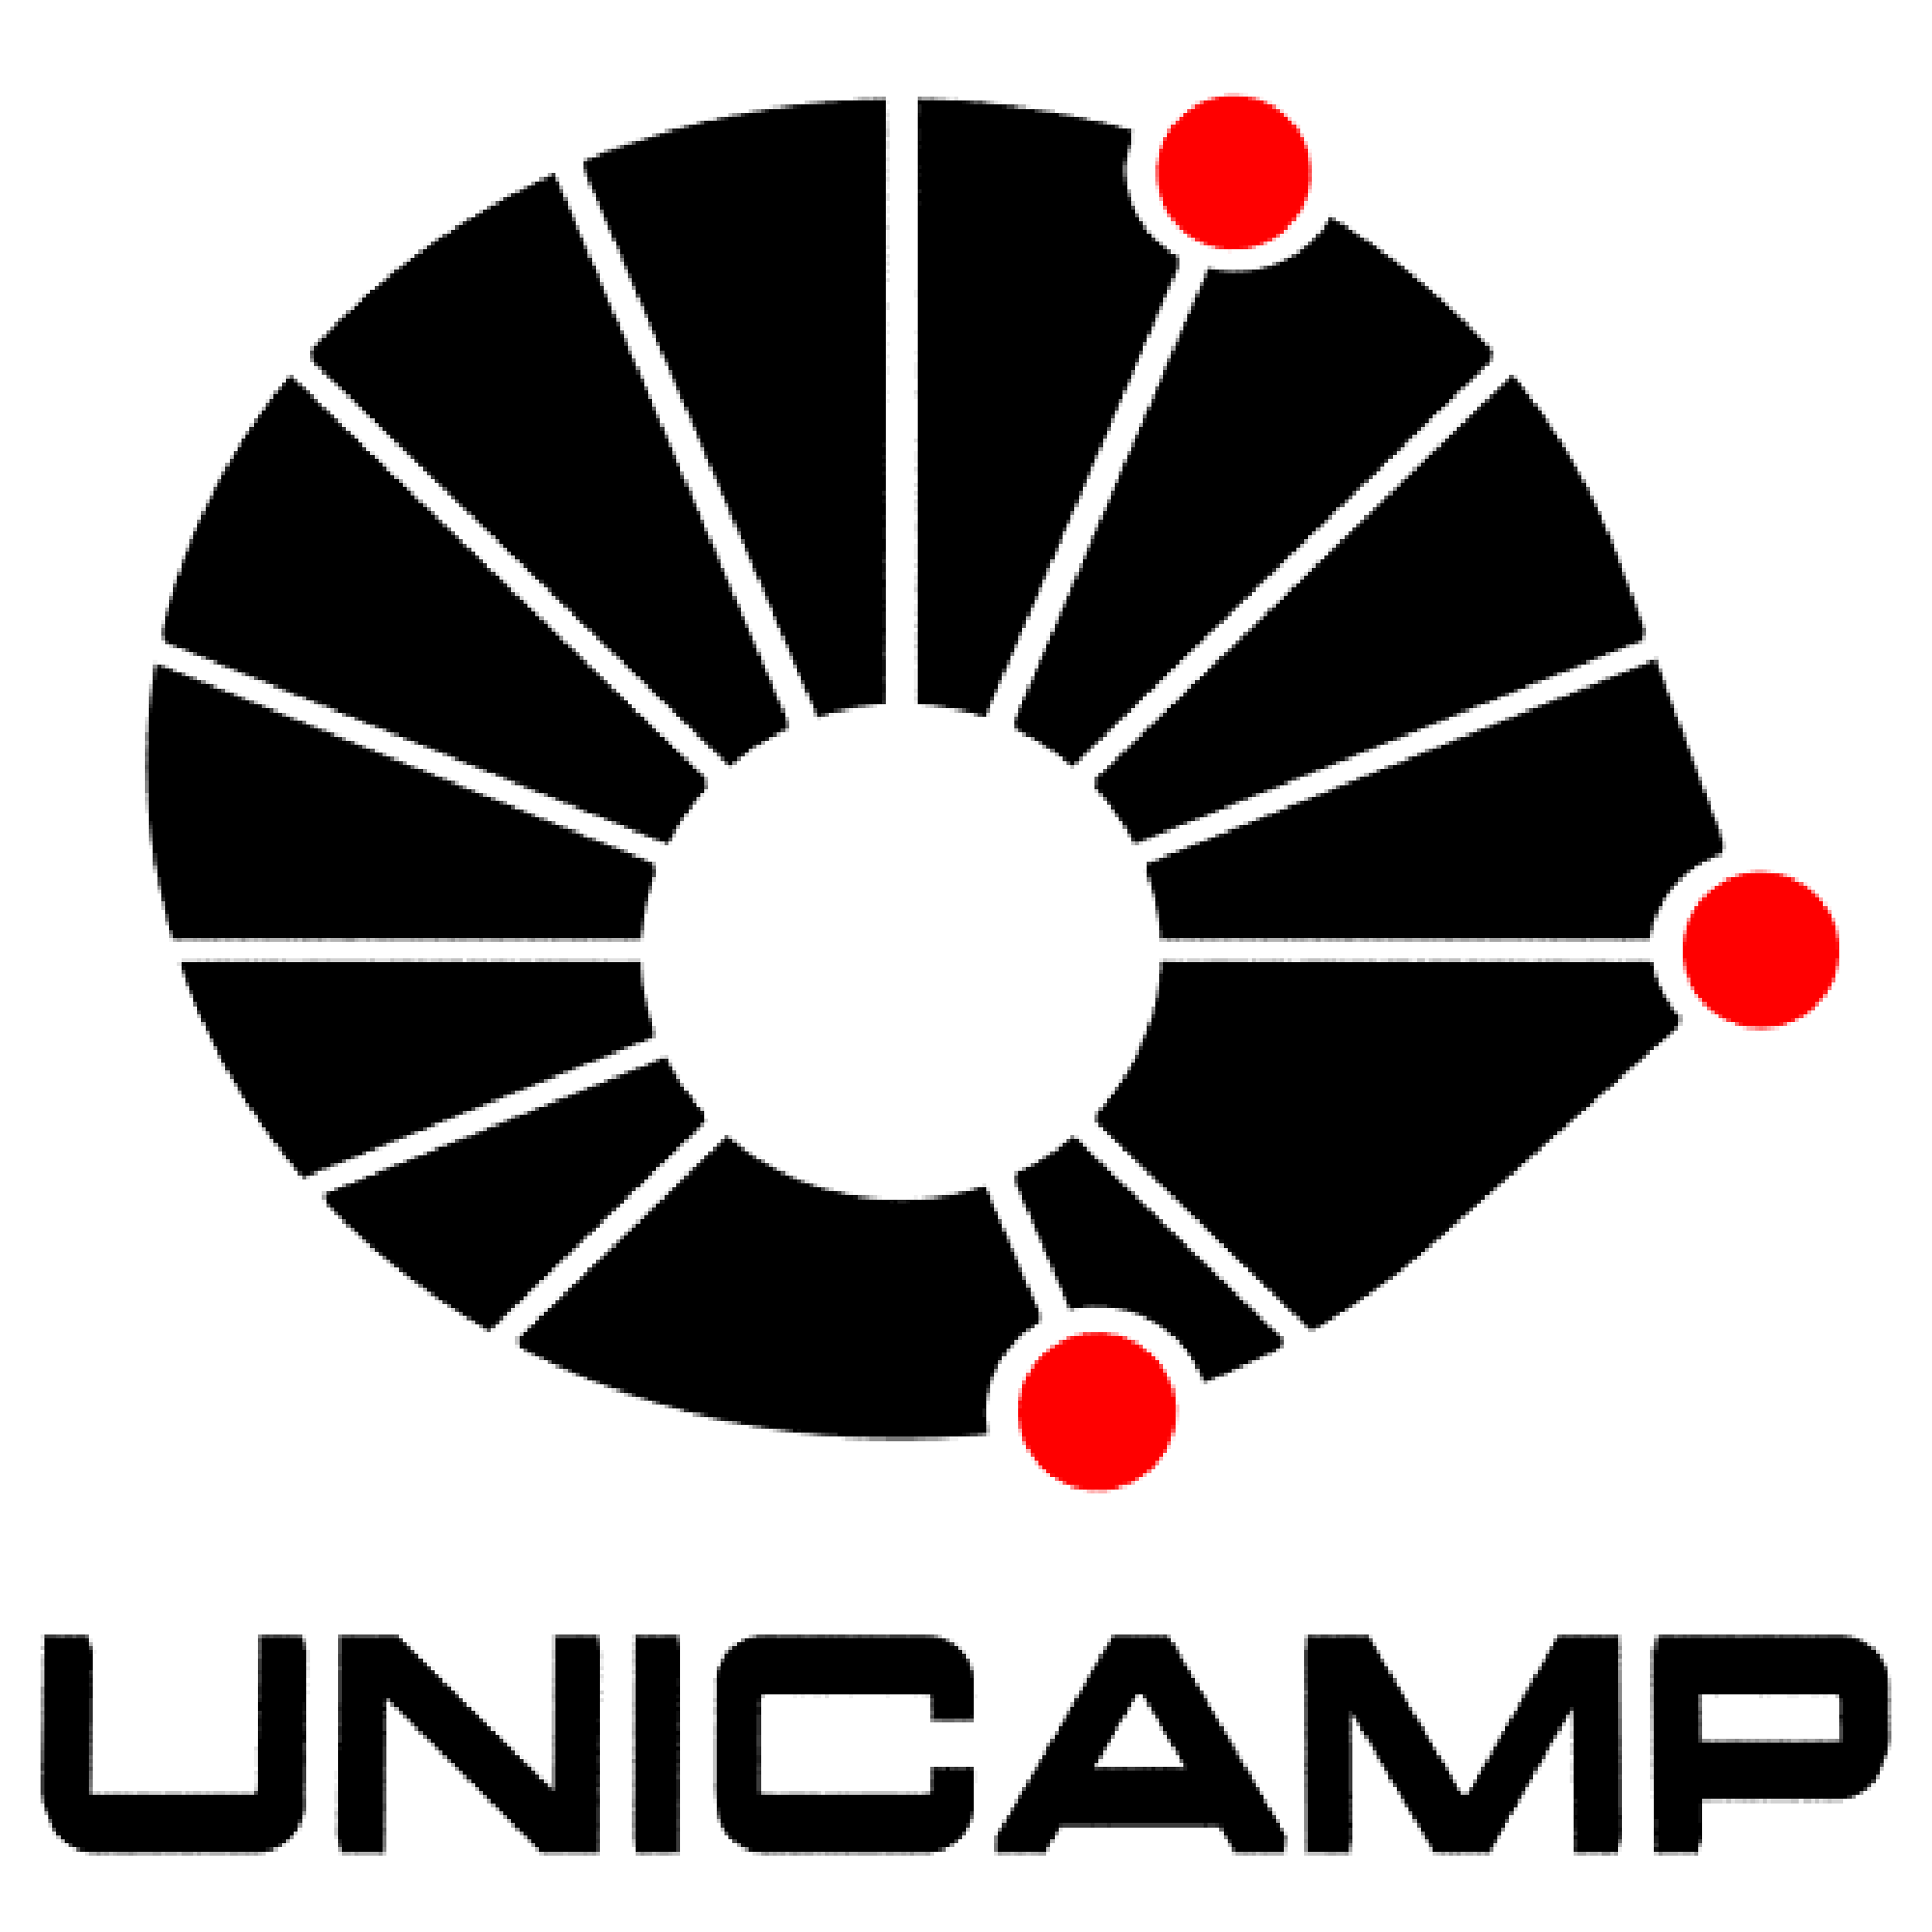
\includegraphics[scale=0.2]{images/logo-unicamp.png}}
% \caption[Shorter figure caption]{Figure Caption caption caption caption
%   caption caption caption caption caption caption caption caption caption
%   caption caption caption caption caption caption caption caption caption
%   caption caption.}
% \label{f:label1}
% \end{figure}
